\subsection{$pp$ 13 TeV}
In 2015 and 2016, low-$\mu$ and intermediate-$\mu$ $pp$ data was collected with ATLAS detectors~\cite{Aad:2008zzm}. An additional pixel layer, the "Insertable B Layer" (IBL)~\cite{atlas:1, atlas:2} installed between Run 1 and Run 2, is used in the $pp$ measurement. There are four run periods depending on the triggers used and they will be discussed in the following sections.

The good events are selected by Good-Run-List and with $|z_{vtx}|<150 $mm.

To reduce the fraction of fake tracks, standard track selection has been applied:
\begin{itemize}
\item Tracks are from primary vertex
\item If IBL hit is expected: at least 1 IBL hit
\item If on IBL hit is expected: a Layer-0 hit if expected
\item At least 1 pixel hit + dead sensors
\item $p_{T}<300$ MeV: at least 2 SCT hits + dead sensors
\item $p_{T}<400$ MeV: at least 4 SCT hits + dead sensors
\item $p_{T}>400$ MeV: at least 6 SCT hits + dead sensors
\item If $p_{T}>10$ GeV: $\chi^{2}$ probability $<0.01$
\item $|d_{0}|<1.5$
\item $|z_{0}-v_{z}|\text{sin}\theta<1.5$
\item $|\eta|\le 2.5$
\item $p_{T}\ge 200$ MeV
\end{itemize}
In the section of systematics, the selection will be tightened to check the stability of the results.



\subsubsection{Run period 1}
Low-$\mu$ data was collected in June and intermediate-$\mu$ data was collected in October. All the runs, with Good Run List (GRL) selections, are included in this analysis and they are listed as below:

\begin{itemize}

\item Run 267358, peak $\mu=0.00255$, 8.6 million events
\begin{itemize}[leftmargin=*]
\item[] \verb|data15_13TeV.00267358.physics_MinBias.merge.AOD.f597_m1441|
\end{itemize}

\item Run 267359, peak $\mu=0.00612$, 12.3 million events
\begin{itemize}[leftmargin=*]
\item[] \verb|data15_13TeV.00267359.physics_MinBias.merge.AOD.f597_m1441|
\end{itemize}

\item Run 267360, peak $\mu=0.374$, 12.6 million events
\begin{itemize}[leftmargin=*]
\item[] \verb|data15_13TeV.00267360.physics_MinBias.merge.AOD.f597_m1441|
\end{itemize}

\item Run 267367, peak $\mu=0.46$, 17.1 million events
\begin{itemize}[leftmargin=*]
\item[] \verb|data15_13TeV.00267367.physics_MinBias.merge.AOD.f597_m1441|
\end{itemize}

\item Run 267385, peak $\mu=0.466$, 71.2 million events
\begin{itemize}[leftmargin=*]
\item[] \verb|data15_13TeV.00267385.physics_MinBias.merge.AOD.f597_m1441|
\end{itemize}

\item Run 267599, peak $\mu=0.488$, 105.6 million events
\begin{itemize}[leftmargin=*]
\item[] \verb|data15_13TeV.00267599.physics_MinBias.merge.AOD.f597_m1441|
\end{itemize}

\item Run 277025, peak $\mu=0.613$, 19.9 million events
\begin{itemize}[leftmargin=*]
\item[] \verb|data15_13TeV.00277025.physics_MinBias.merge.AOD.f624_m1486|
\end{itemize}

\item Run 277081, peak $\mu=0.62$, 44.5 million events
\begin{itemize}[leftmargin=*]
\item[] \verb|data15_13TeV.00277081.physics_MinBias.merge.AOD.f624_m1486|
\end{itemize}

\end{itemize}
where peak $\mu$ is the highest $\mu$ value during data taking.

The triggers~\cite{Aad:2012xs} that have been used in this analysis have both minimum bias (MinBias) and high multiplicity track (HMT) triggers~\cite{Aaboud:2016yar, Aad:2016mok} The HMT triggers are developed to enhance the statistics in high multiplicity region. Since the main uncertainty in cumulant analysis is from statistical errors, HMT triggers are crucial in order to extend the measurement to higher multiplicity region. This is especially more important in sub-event method, since not all the particles pairs are included. The list of all triggers used in this run period are listed as follows:
\begin{itemize}
\item \verb|HLT_noalg_mb_L1MBTS_1|
\item \verb|HLT_mb_sp400_trk40_hmt_L1MBTS_1_1|
\item \verb|HLT_mb_sp700_trk50_hmt_L1MBTS_1_1|
\item \verb|HLT_mb_sp900_trk60_hmt_L1MBTS_1_1|
\item \verb|HLT_mb_sp1400_trk90_hmt_L1TE10|
\end{itemize}
where the items of the triggers are explained below:
\begin{itemize}
\item \verb|L1MBTS_1|: L1 trigger requires at least 1 hit at either side of MBTS detector;
\item \verb|L1MBTS_1_1|: L1 trigger requires at least 1 hit at both side of MBTS detector;
\item \verb|L1TEX|: L1 trigger is seeded at L1 total energy from the full $\eta$ range and the threshold is X GeV;
\item \verb|spX|: HLT trigger requires X number of space points in the SCT detector;
\item \verb|trkX|: HLT trigger requires X number of online reconstructed tracks from primary vertex;
\end{itemize}

\begin{figure}[H]
\centering
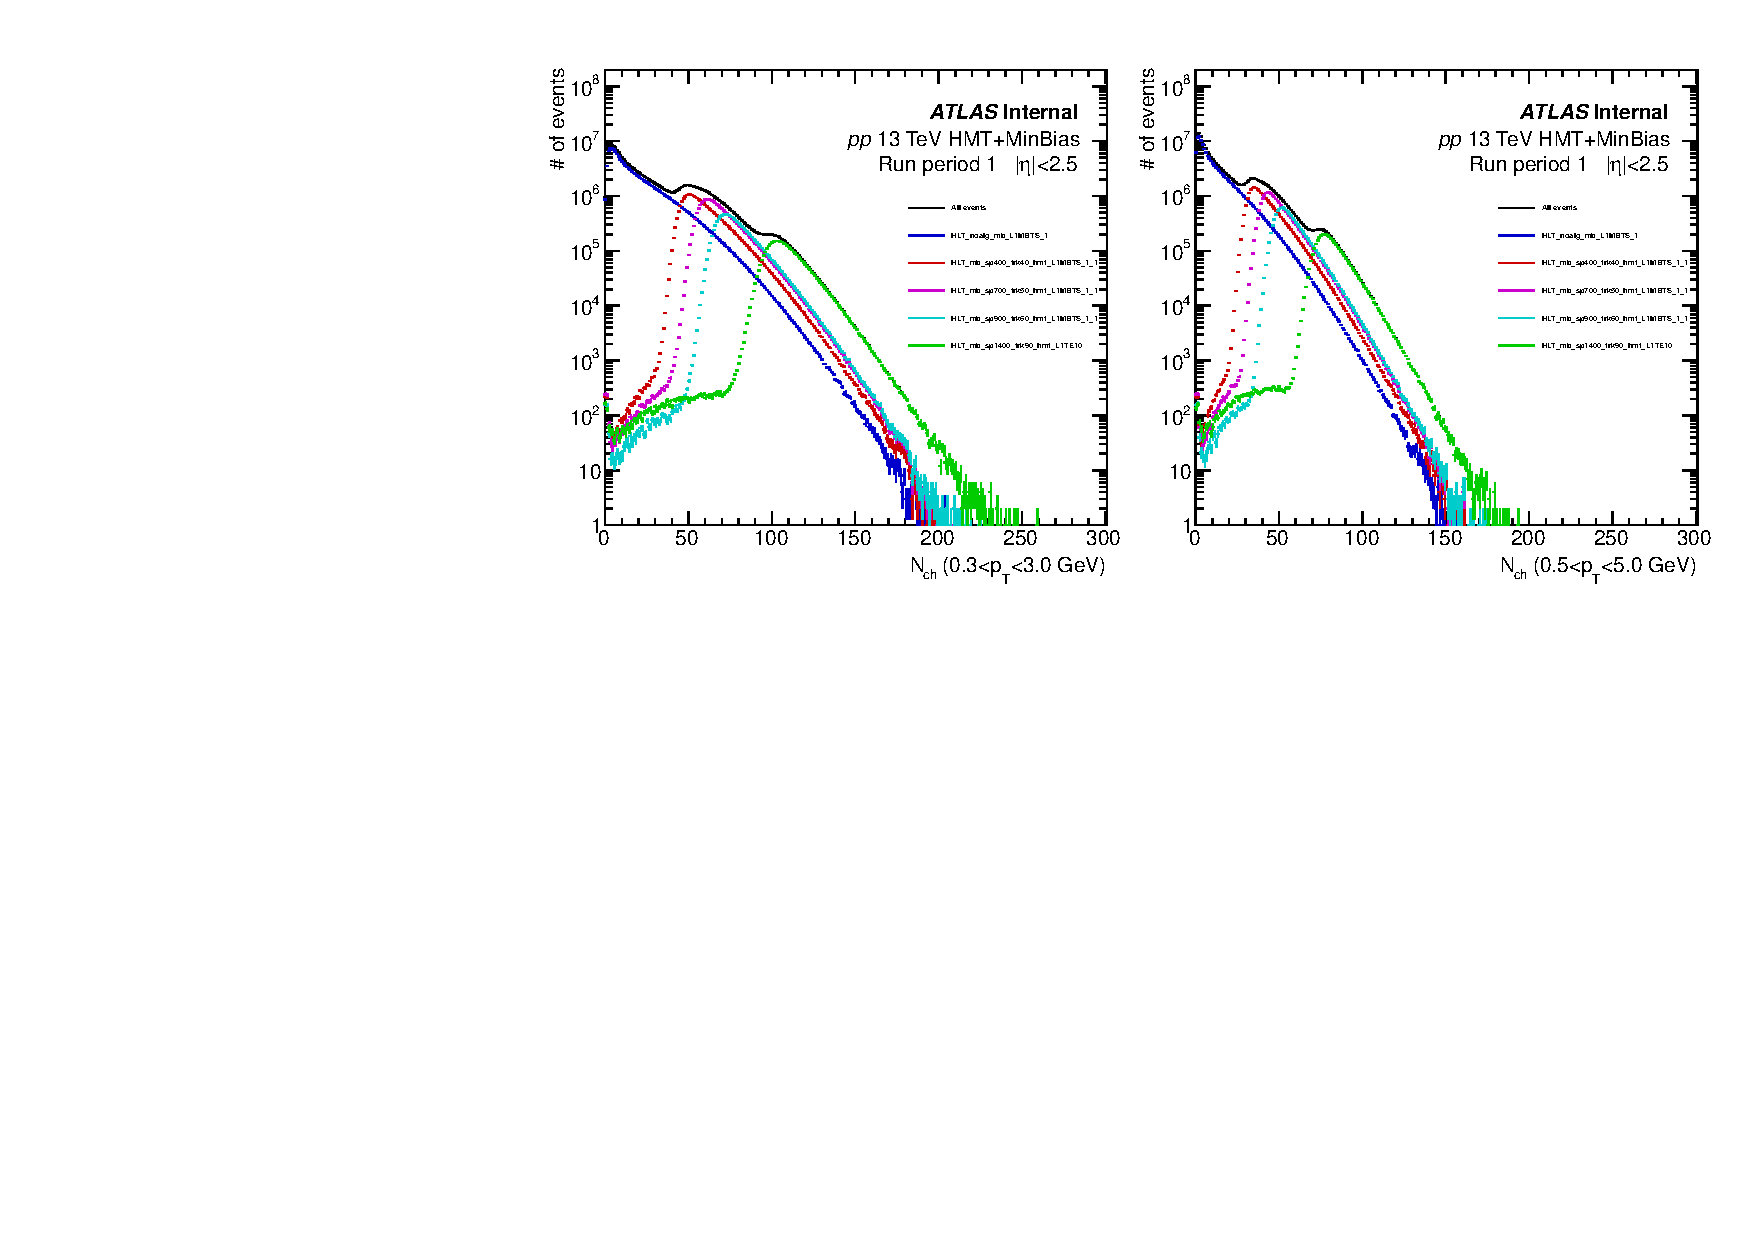
\includegraphics[width=.9\linewidth]{figs/sec_evtSlc/trkDis_pp13_run1.pdf}
\caption{Distribution of number of tracks with two $p_{T}$ thresholds: $0.3<p_{T}<3.0$ GeV and $0.5<p_{T}<5.0$ GeV, in 13 TeV $pp$ run period 1. The major MinBias and HMT triggers are plotted separately. "All events" means all the MinBias and HMT triggers included, mainly from L1TE and HMT performance triggers.}
\label{fig:trkDis_pp13_run1}
\end{figure}

As a summary of total statistics with all runs combined, Fig.\ref{fig:trkDis_pp13_run1} shows the distributions of number of tracks with two $p_{T}$ cuts used in this analysis: $0.3<p_{T}<3.0$ GeV and $0.5<p_{T}<5.0$ GeV. In each case, events collected with different MinBias and HMT triggers are shown separately, since in the end we will apply lower $N_{ch}$ cuts to reduce the selection bias introduced by HMT triggers. Statistics of all the triggers in the MinBias stream (including those triggers not used in this analysis) are listed in the Appendix.

\begin{figure}[H]
\centering
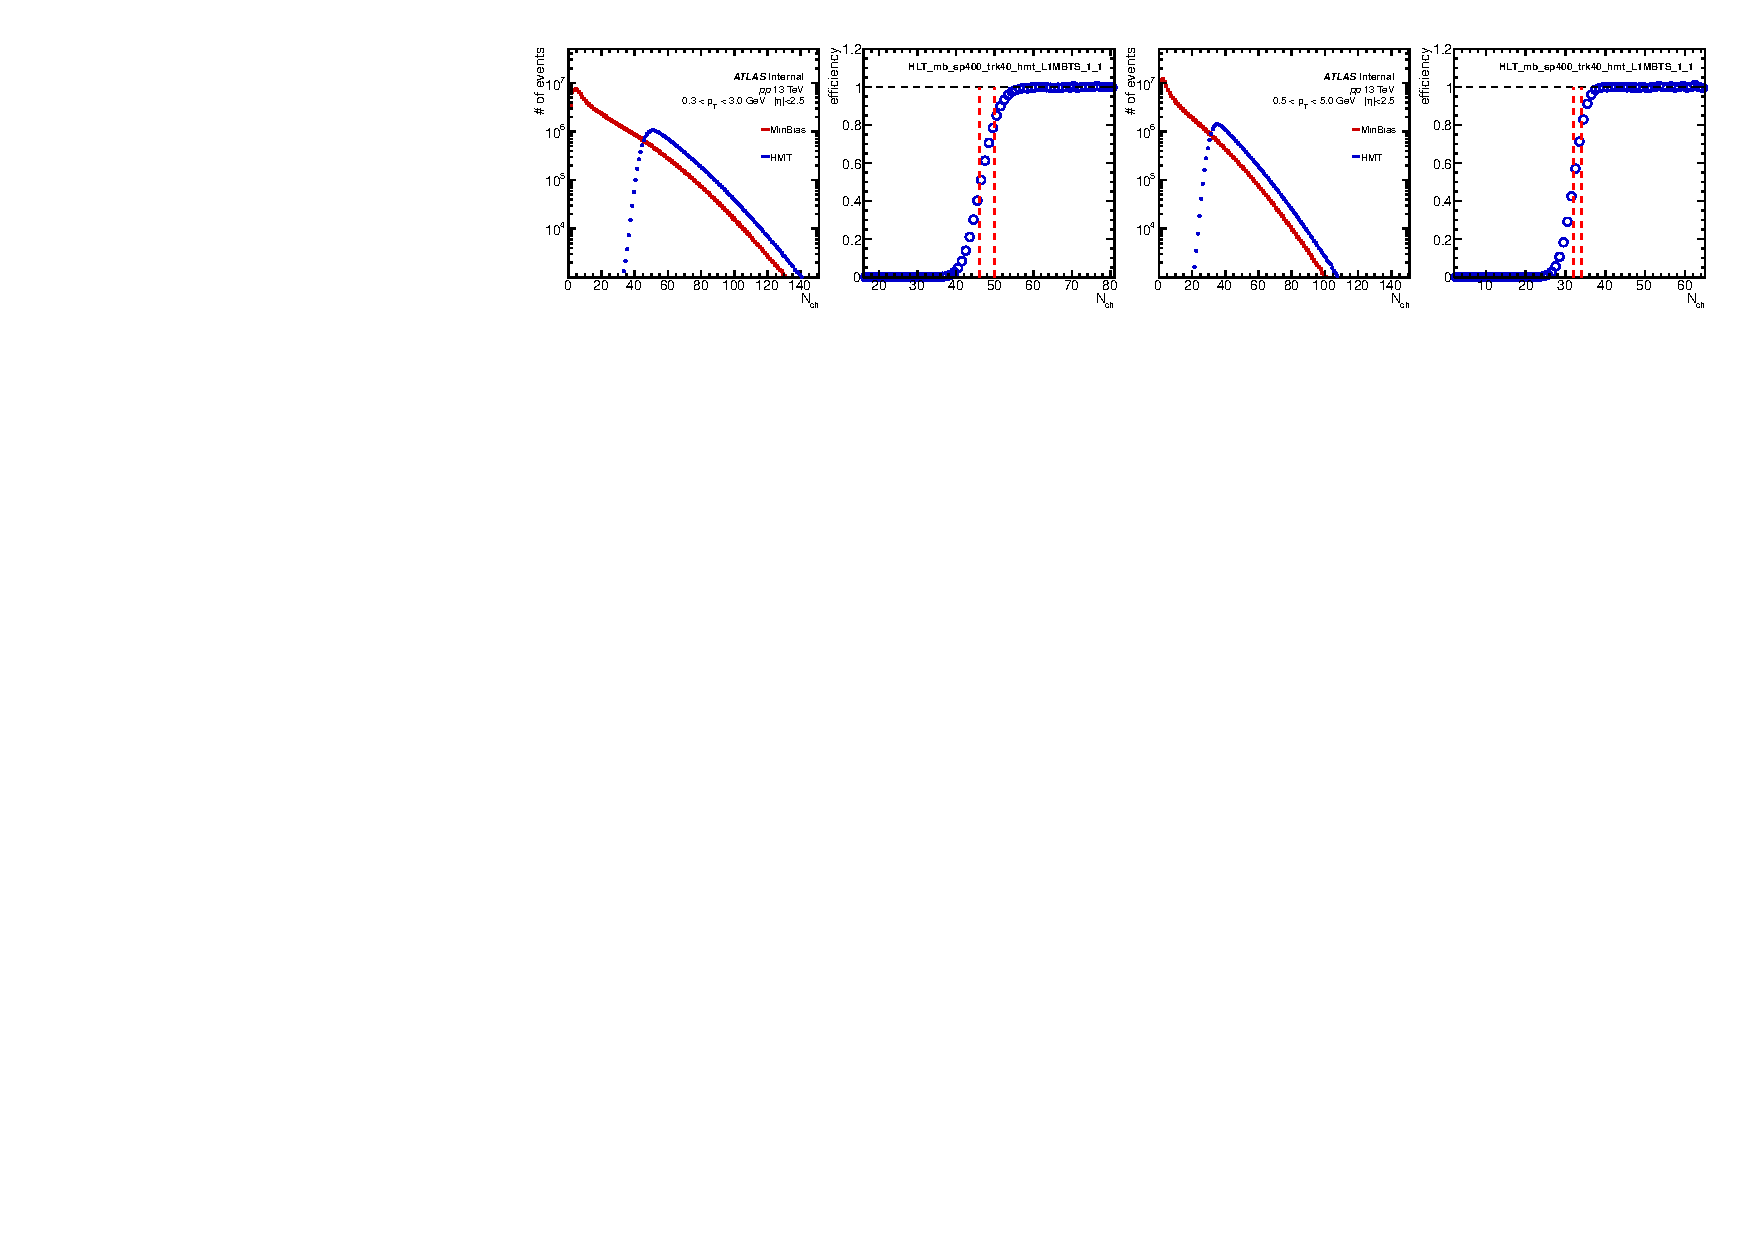
\includegraphics[width=1.\linewidth]{figs/sec_evtSlc/trigEff_pp13_run1/trigEff_Trig11.pdf}
\end{figure}
\begin{figure}[H]
\centering
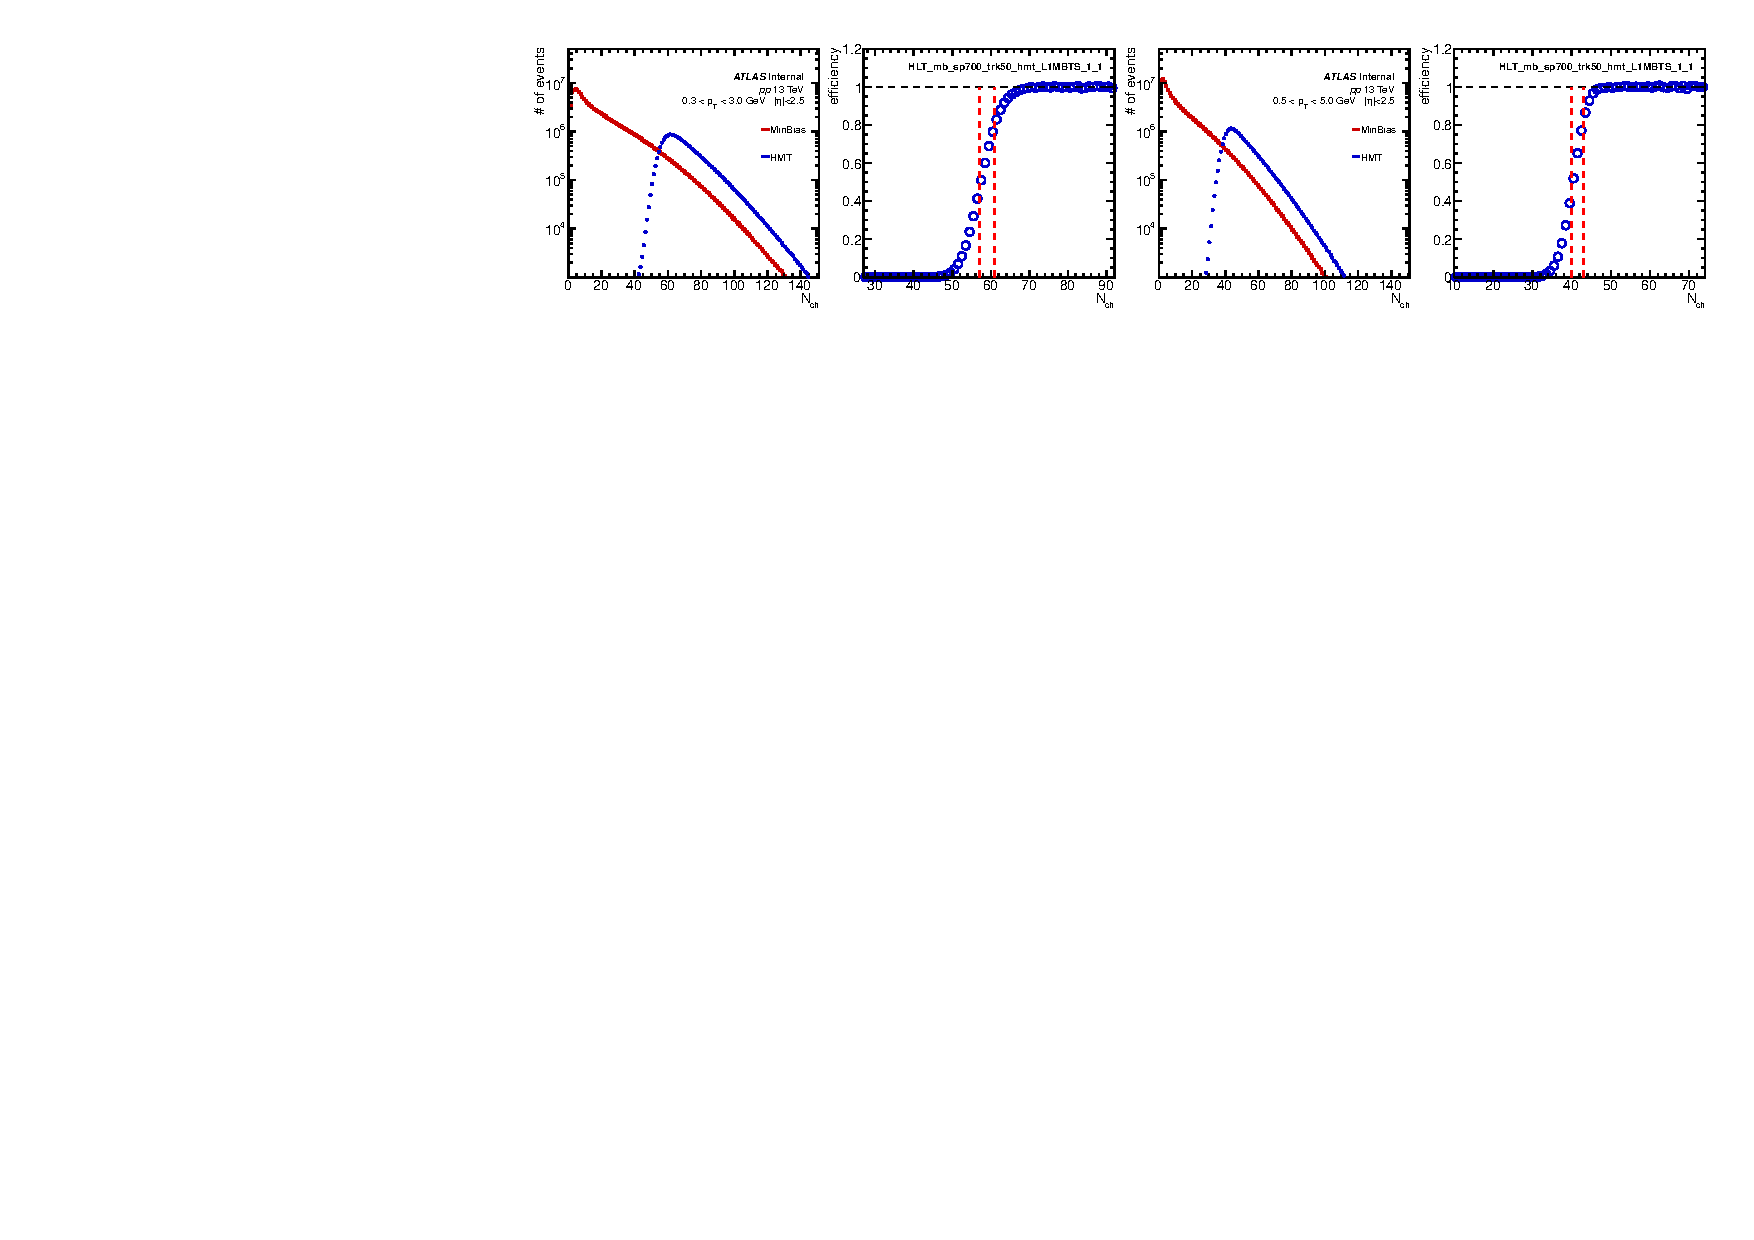
\includegraphics[width=1.\linewidth]{figs/sec_evtSlc/trigEff_pp13_run1/trigEff_Trig12.pdf}
\end{figure}
\begin{figure}[H]
\centering
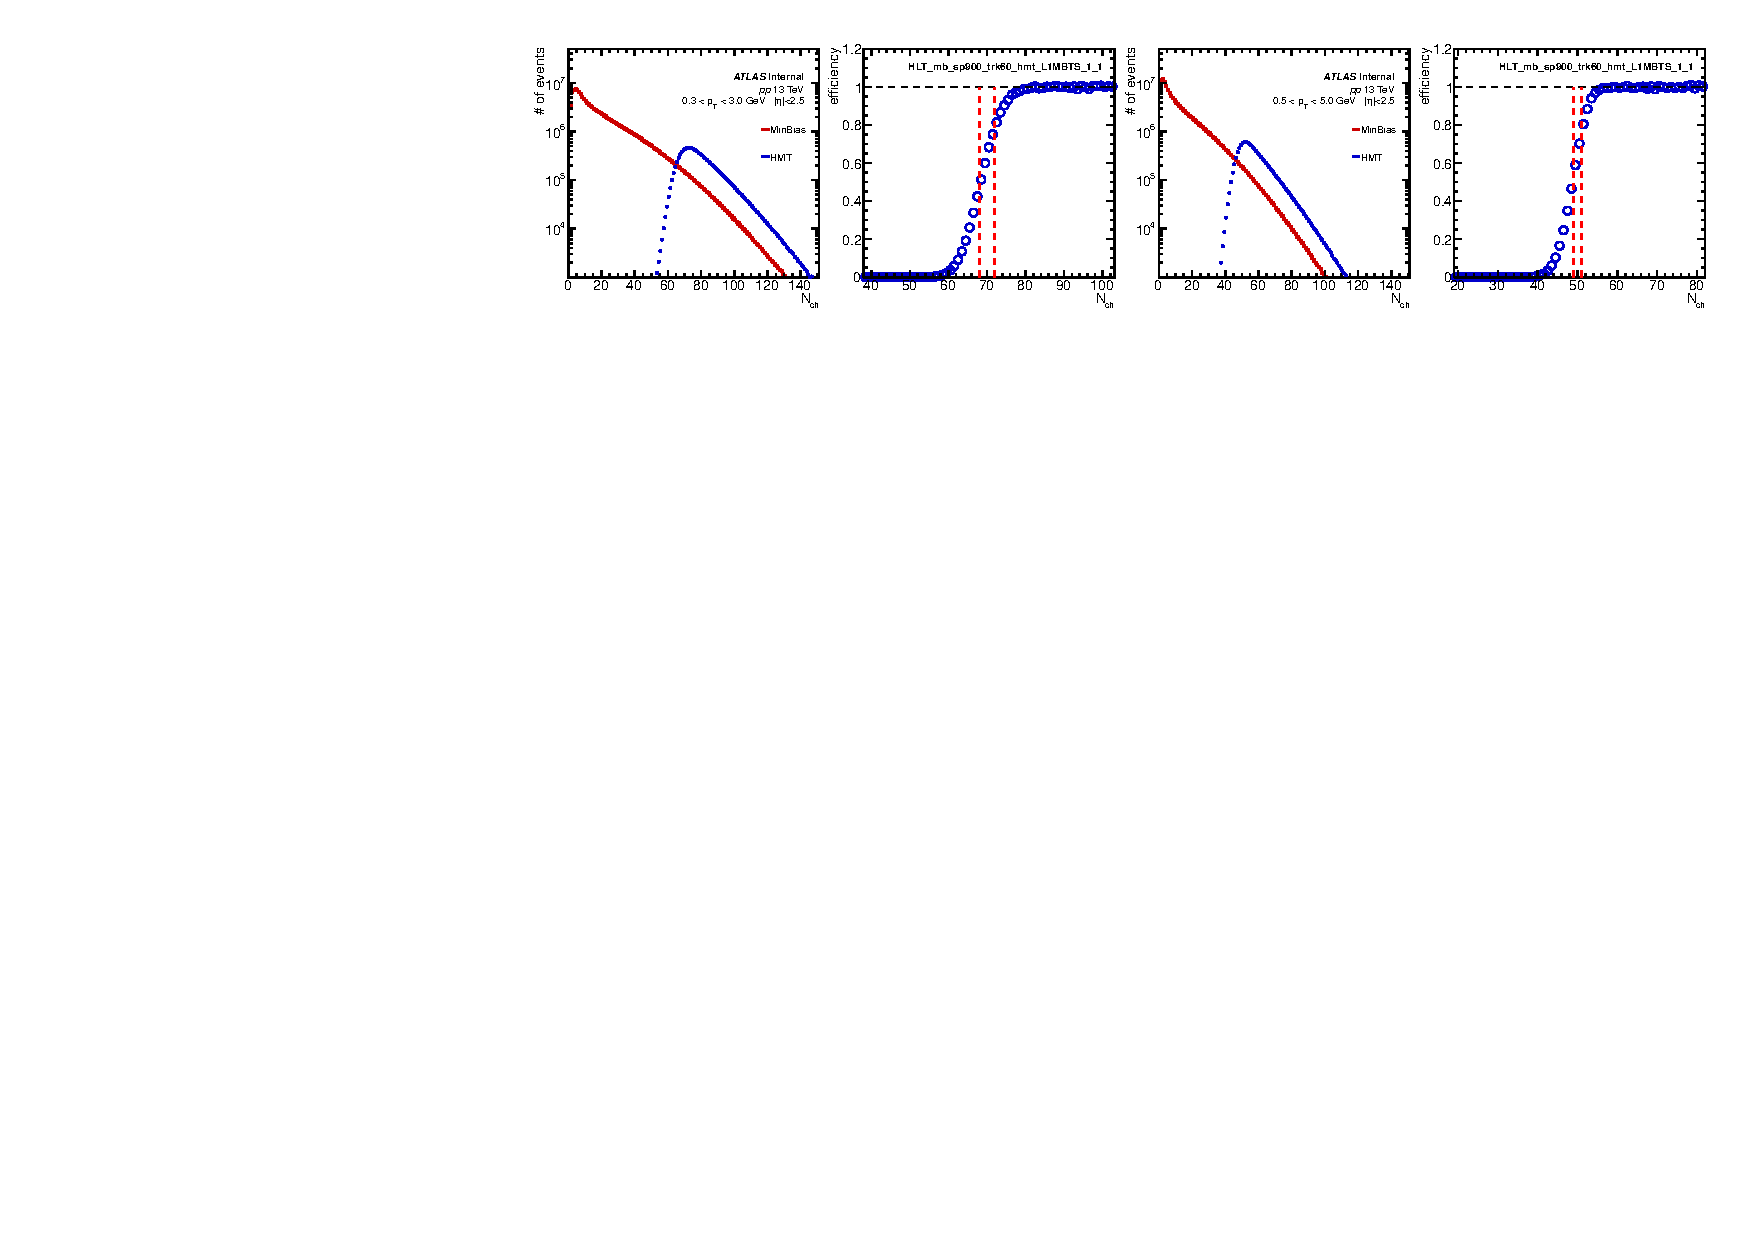
\includegraphics[width=1.\linewidth]{figs/sec_evtSlc/trigEff_pp13_run1/trigEff_Trig13.pdf}
\end{figure}
\begin{figure}[H]
\centering
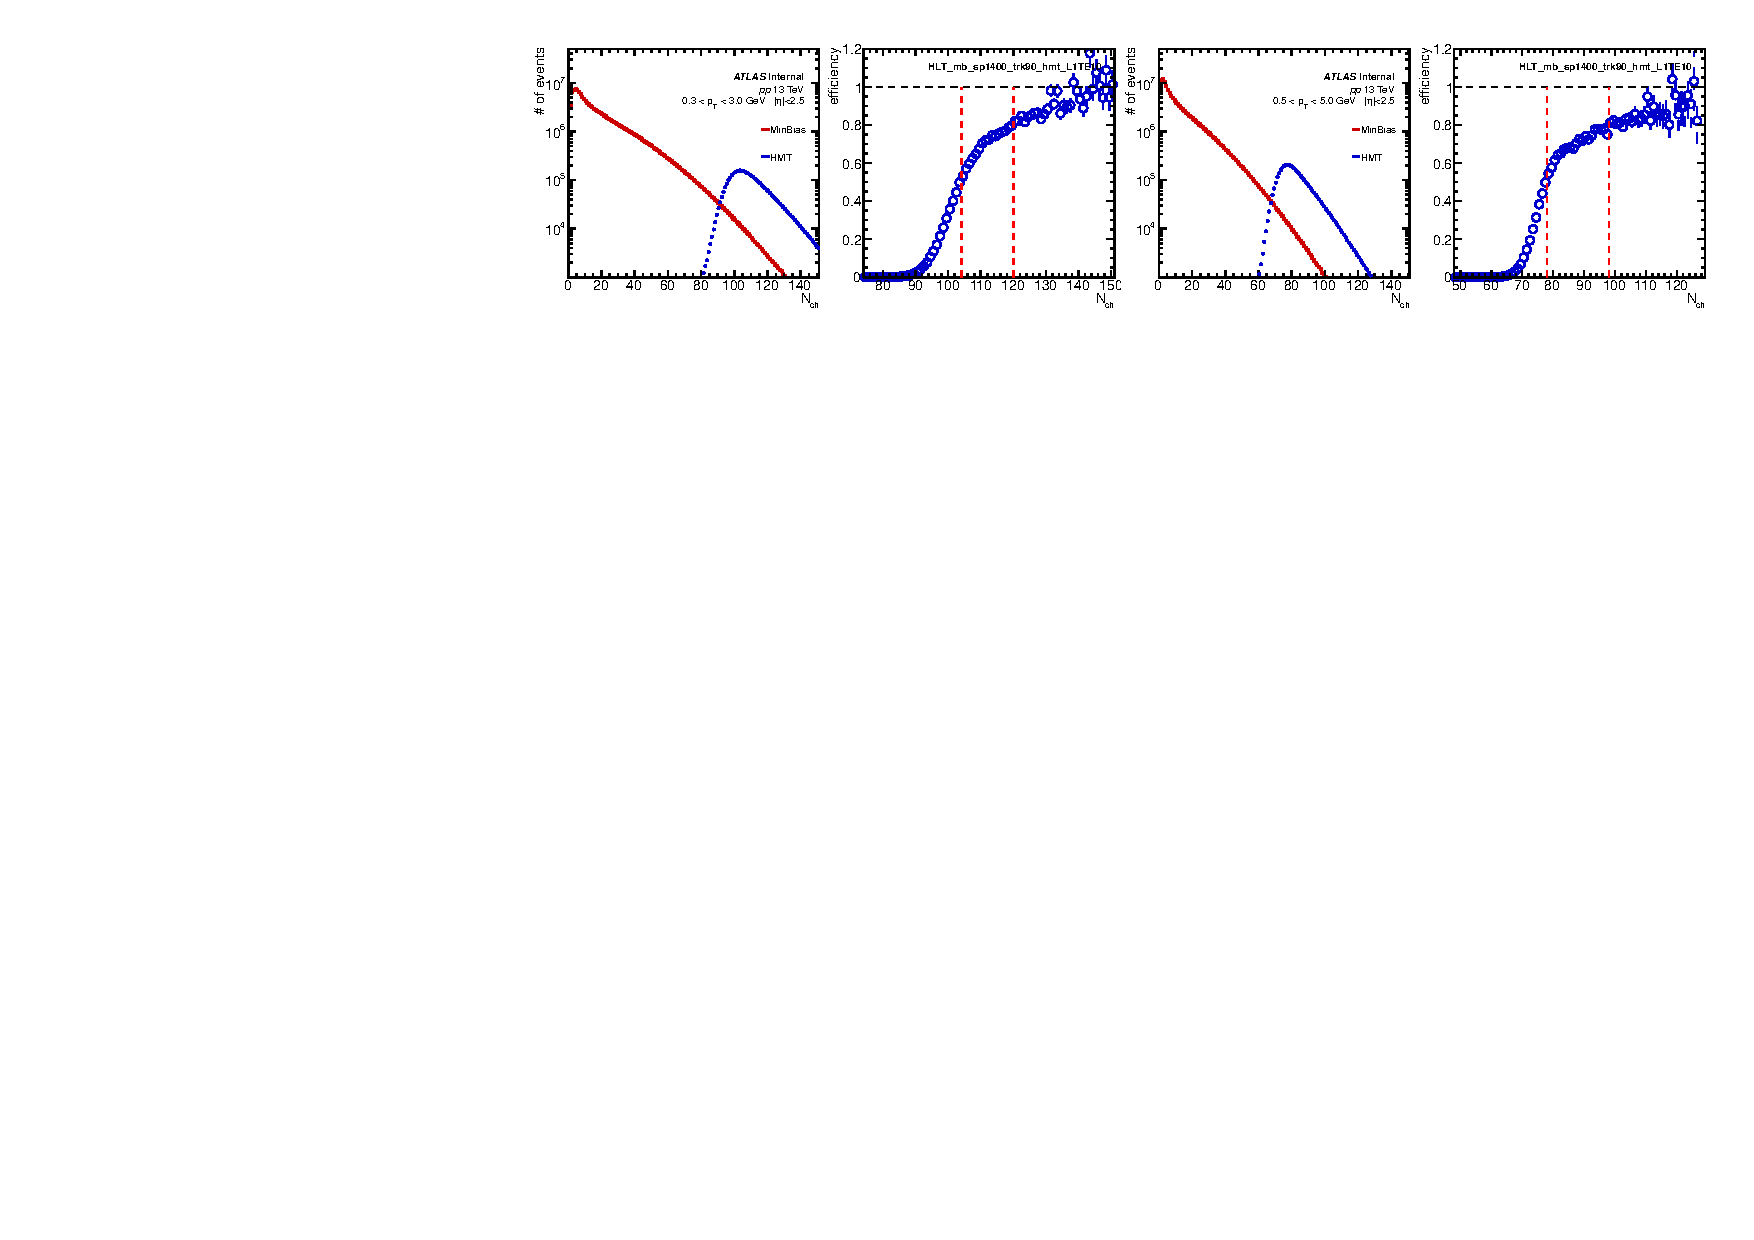
\includegraphics[width=1.\linewidth]{figs/sec_evtSlc/trigEff_pp13_run1/trigEff_Trig15.pdf}
\caption{Trigger efficiencies of all major HMT triggers as a function of number of tracks in two $p_{T}$ ranges: $0.3<p_{T}<3.0$ GeV and $0.5<p_{T}<5.0$ GeV, from 13 TeV $pp$ run period 1. Efficiency is calculated relative to the corresponding MinBias trigger in this run period then scaled to 1.0 in the large $N_{ch}$ region. The two red dash lines indicate 50$\%$ and 80$\%$ efficiency cuts.}
\label{fig:trigEff_pp13_run1}
\end{figure}
During the data taking, both minbias and HMT triggers are prescaled. The triggers efficiency $\epsilon$ is estimated on the statistical level:
\begin{equation}
\epsilon^{\text{HMT}}\equiv\frac{\text{number of events passed HMT trigger}*\text{PS of HMT trigger}}{\text{number of events passed MB trigger}*\text{PS of MB trigger}}
\end{equation}
Since the number of events with high $N_{ch}$ triggered by minbias trigger is limited (during some runs the prescale of minbias triggers are very high), the estimated HMT trigger efficiency could fluctuate around $1$ in some cases. However, because the turn-on of HMT trigger is very sharp, $N_{ch}$ cut with $50\%$ and $80\%$ efficiency are not affected by this estimation. Trigger efficiencies of all the major HMT triggers are summarized in Fig.~\ref{fig:trigEff_pp13_run1}, where efficiencies are shown for two $p_{T}$ ranges separately: $0.3<p_{T}<3.0$ GeV and $0.5<p_{T}<5.0$ GeV. In order to remove the potential bias introduced by trigger selections, HMT events are only used when their corresponding trigger efficiency is larger than 50$\%$. Another criteria of larger than 80$\%$ is applied as a cross check and will be included as one of the systematics.



\subsubsection{Run period 2}
The 2nd run period data was taken in 2016 and there are 2 runs used for this analysis:
\begin{itemize}

\item Run 299390, peak $\mu=0.052$, 4.1 million events
\begin{itemize}[leftmargin=*]
\item[] \verb|data16_13TeV.00299390.physics_MinBias.recon.AOD.r8358/|
\end{itemize}

\item Run 300287, peak $\mu=0.052$, 8.1 million events
\begin{itemize}[leftmargin=*]
\item[] \verb|data16_13TeV.00300287.physics_MinBias.recon.AOD.r8358/|
\end{itemize}

\end{itemize}
The major MinBias and HMT triggers applied in this run period are:
\begin{itemize}
\item \verb|HLT_noalg_mb_L1MBTS_1_1|
\item \verb|HLT_mb_sp1800_hmtperf_L1TE5|
\item \verb|HLT_mb_sp1500_hmtperf_L1TE10|
\item \verb|HLT_mb_sp900_trk60_hmt_L1MBTS_1_1|
\item \verb|HLT_mb_sp1000_trk70_hmt_L1TE5|
\item \verb|HLT_mb_sp1400_trk90_hmt_L1TE10|
\end{itemize}
where there is one new trigger item:
\begin{itemize}
\item \verb|hmt_perf|: performance triggers of HMT, usually without online track cuts;
\end{itemize}

\begin{figure}[H]
\centering
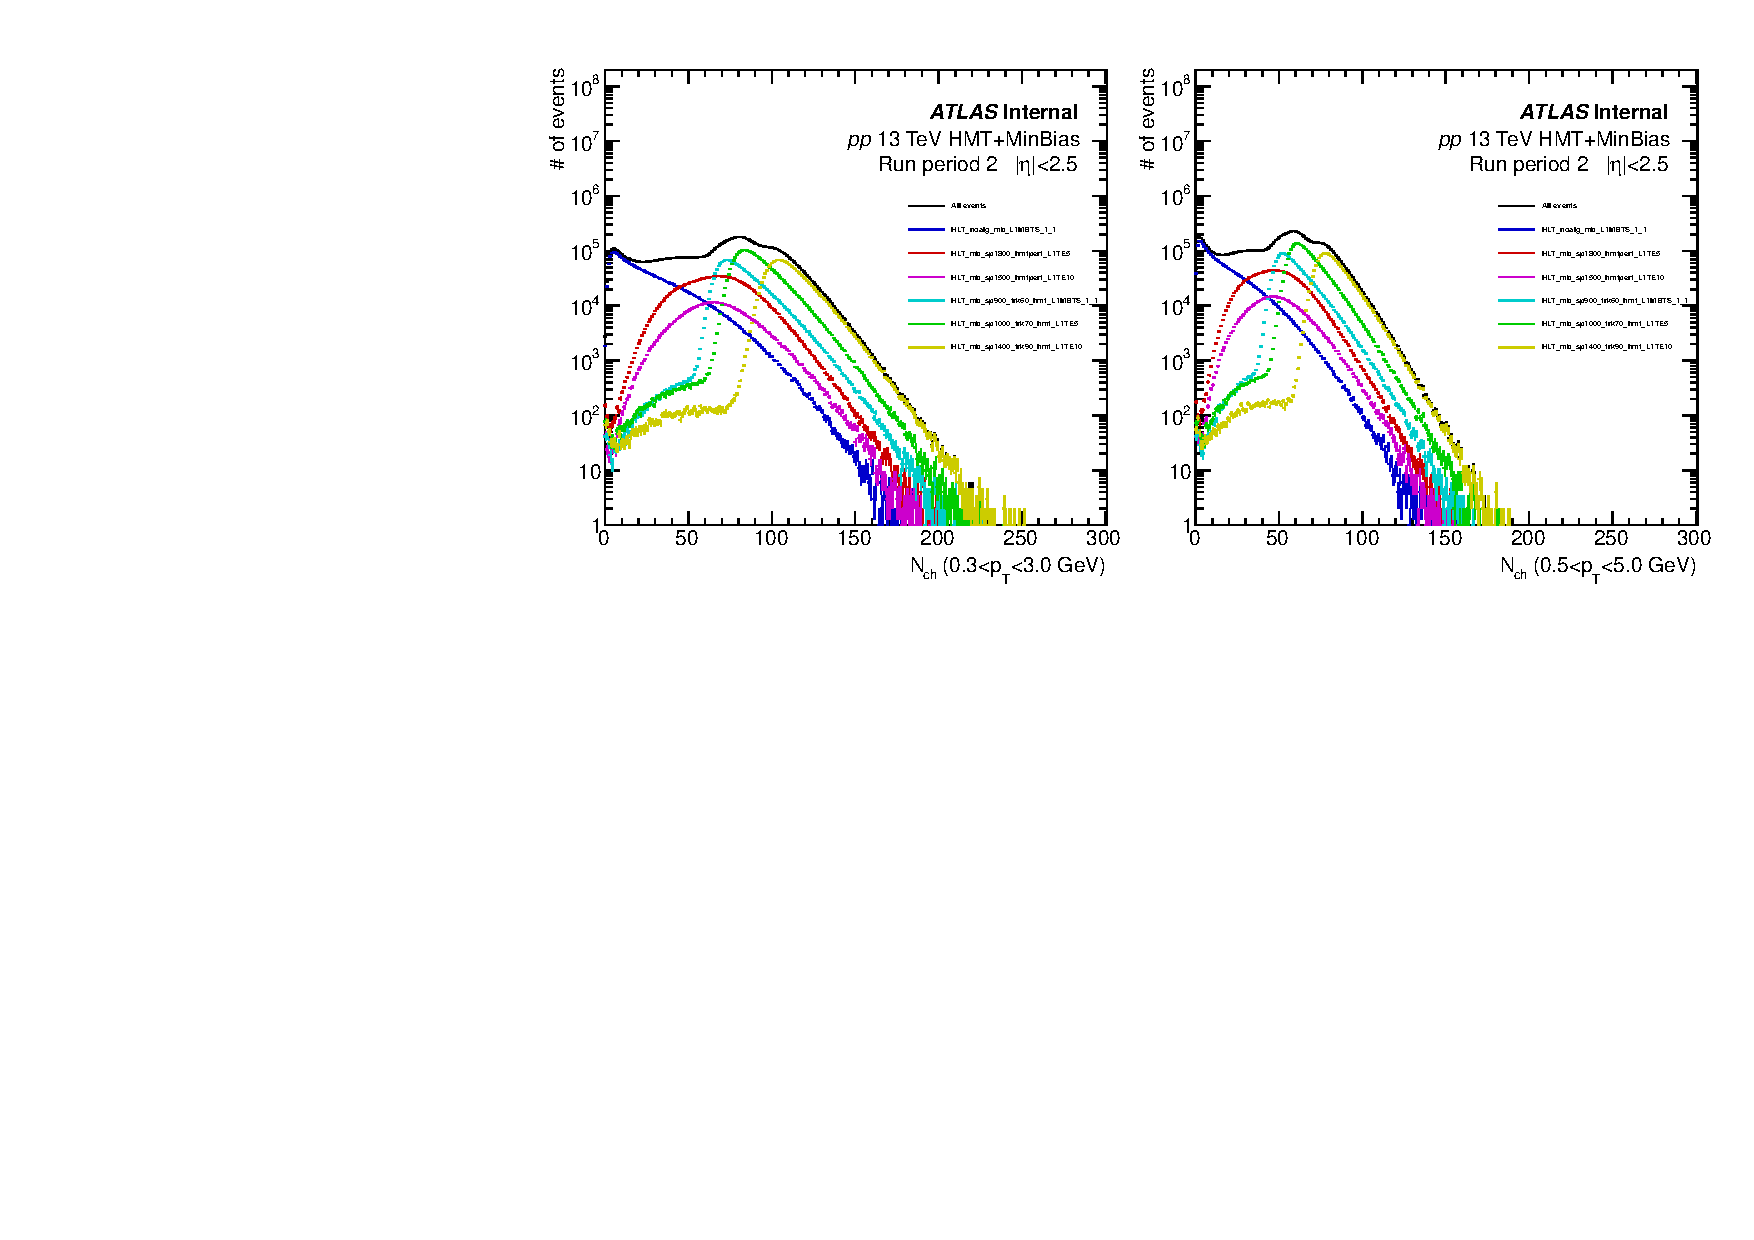
\includegraphics[width=.9\linewidth]{figs/sec_evtSlc/trkDis_pp13_run2.pdf}
\caption{Distribution of number of tracks with two $p_{T}$ thresholds: $0.3<p_{T}<3.0$ GeV and $0.5<p_{T}<5.0$ GeV, in 13 TeV $pp$ run period 2. The major MinBias and HMT triggers are plotted separately.}
\label{fig:trkDis_pp13_run2}
\end{figure}
The summary of statistics with all the major triggers used in this analysis are shown in Fig.~\ref{fig:trkDis_pp13_run2}.

\begin{figure}[H]
\centering
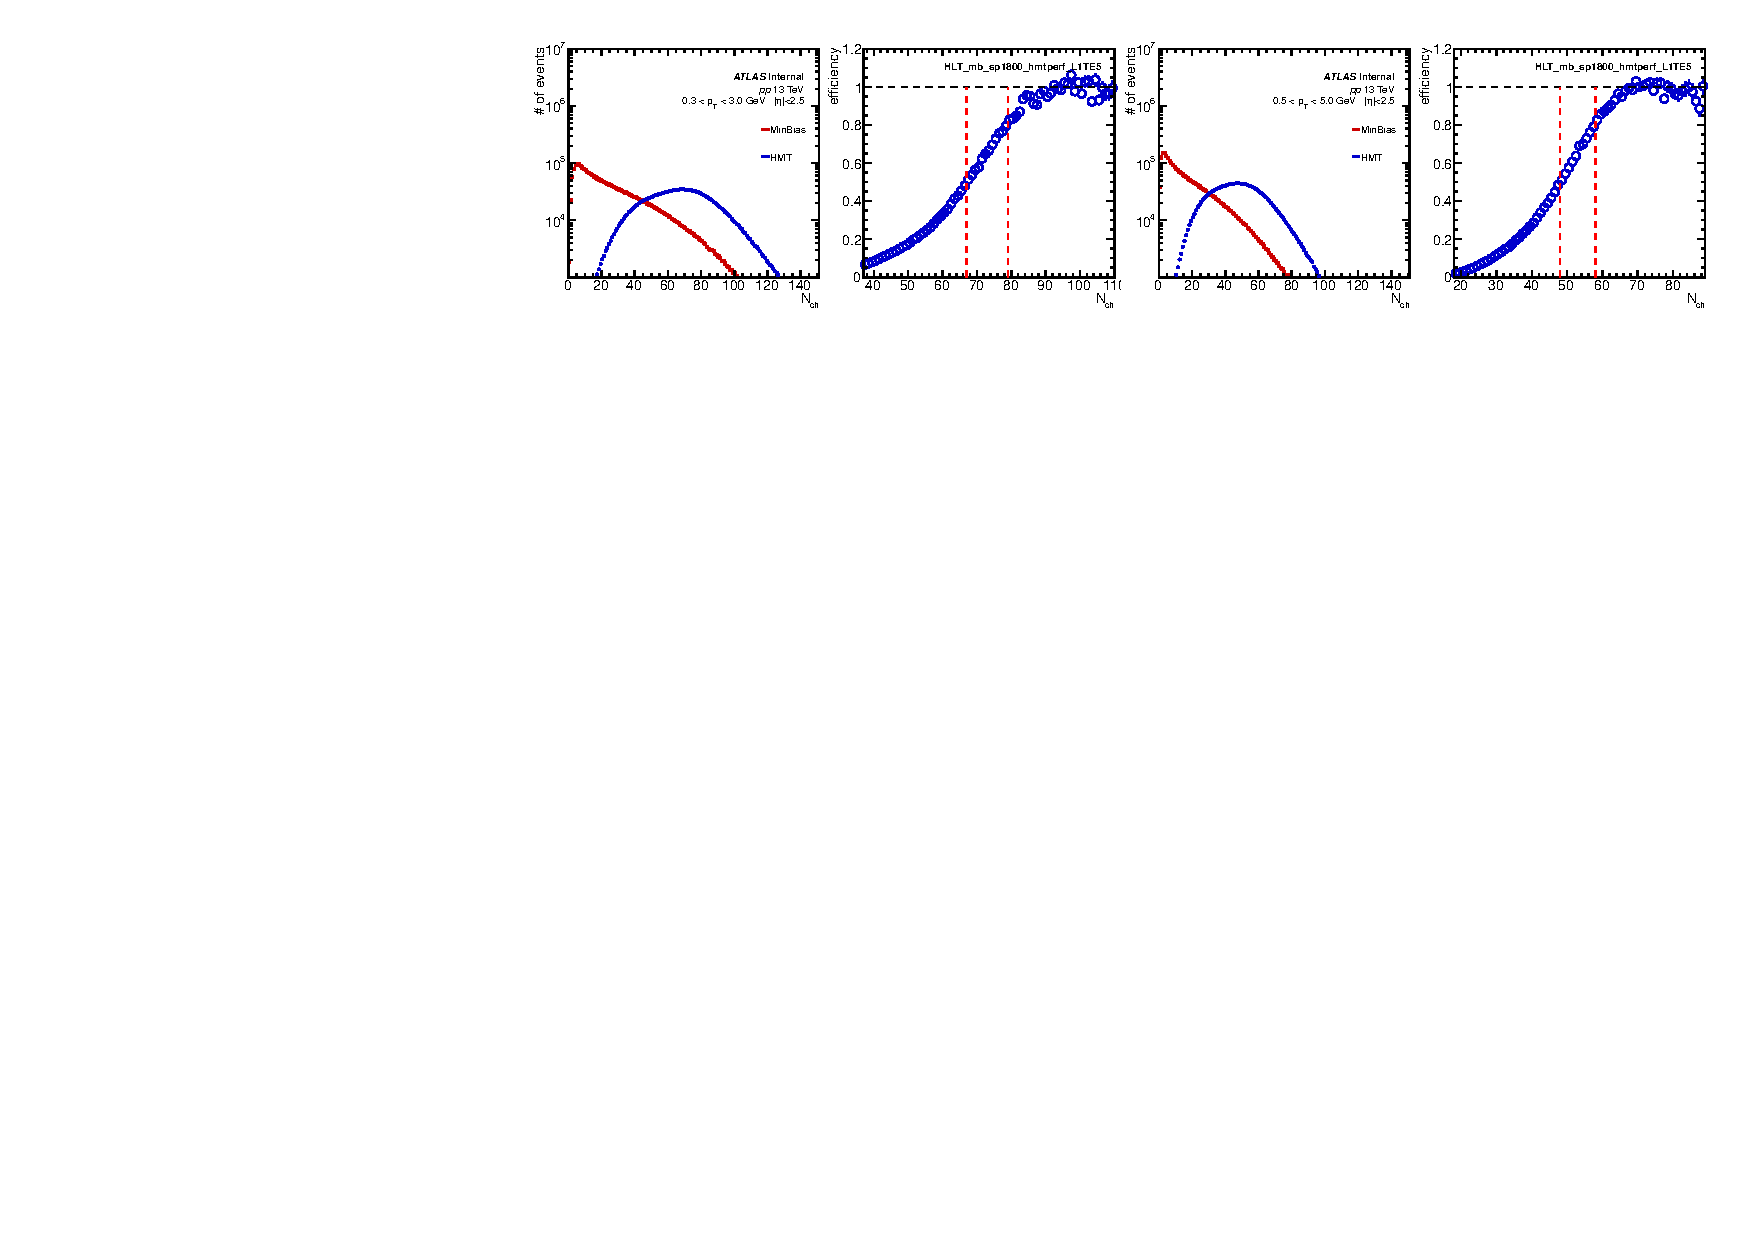
\includegraphics[width=1.\linewidth]{figs/sec_evtSlc/trigEff_pp13_run2/trigEff_Trig17.pdf}
\end{figure}
\begin{figure}[H]
\centering
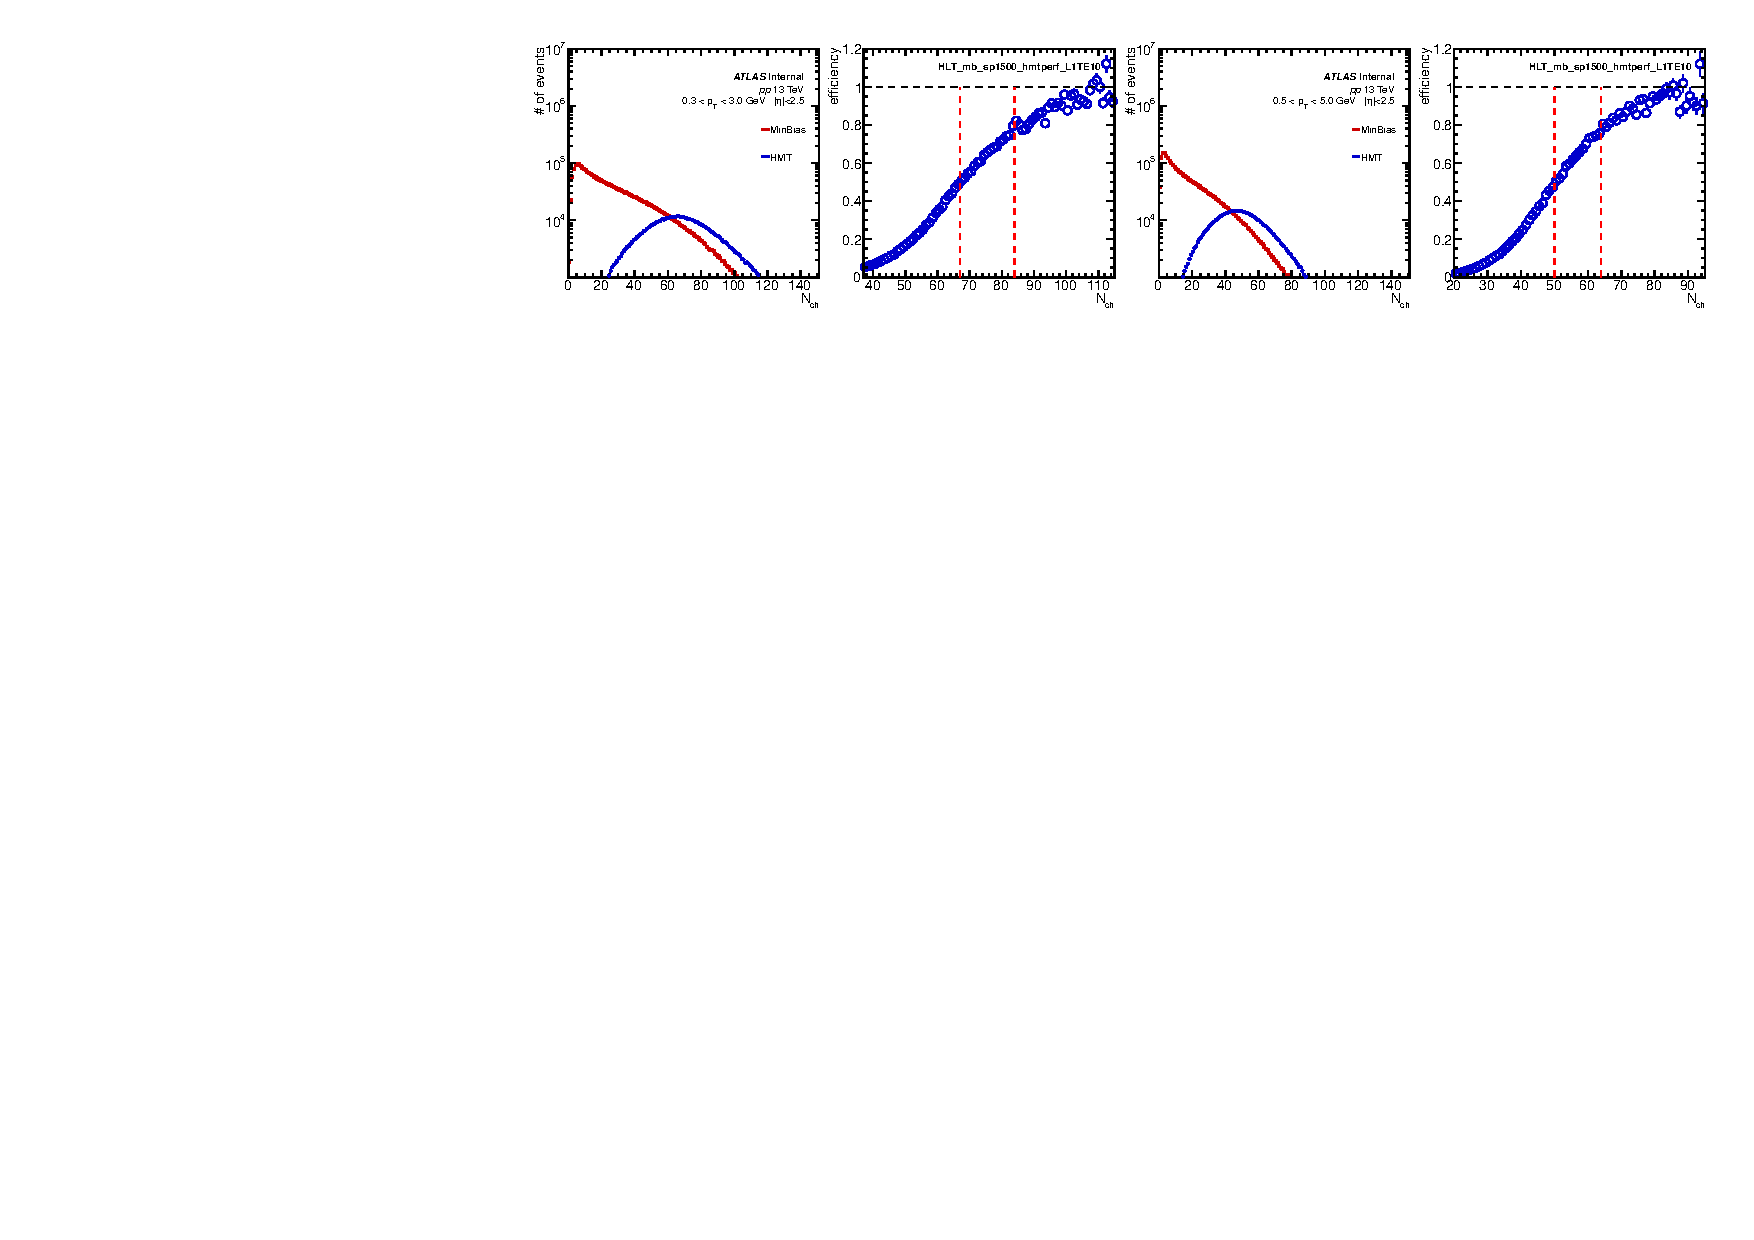
\includegraphics[width=1.\linewidth]{figs/sec_evtSlc/trigEff_pp13_run2/trigEff_Trig18.pdf}
\end{figure}
\begin{figure}[H]
\centering
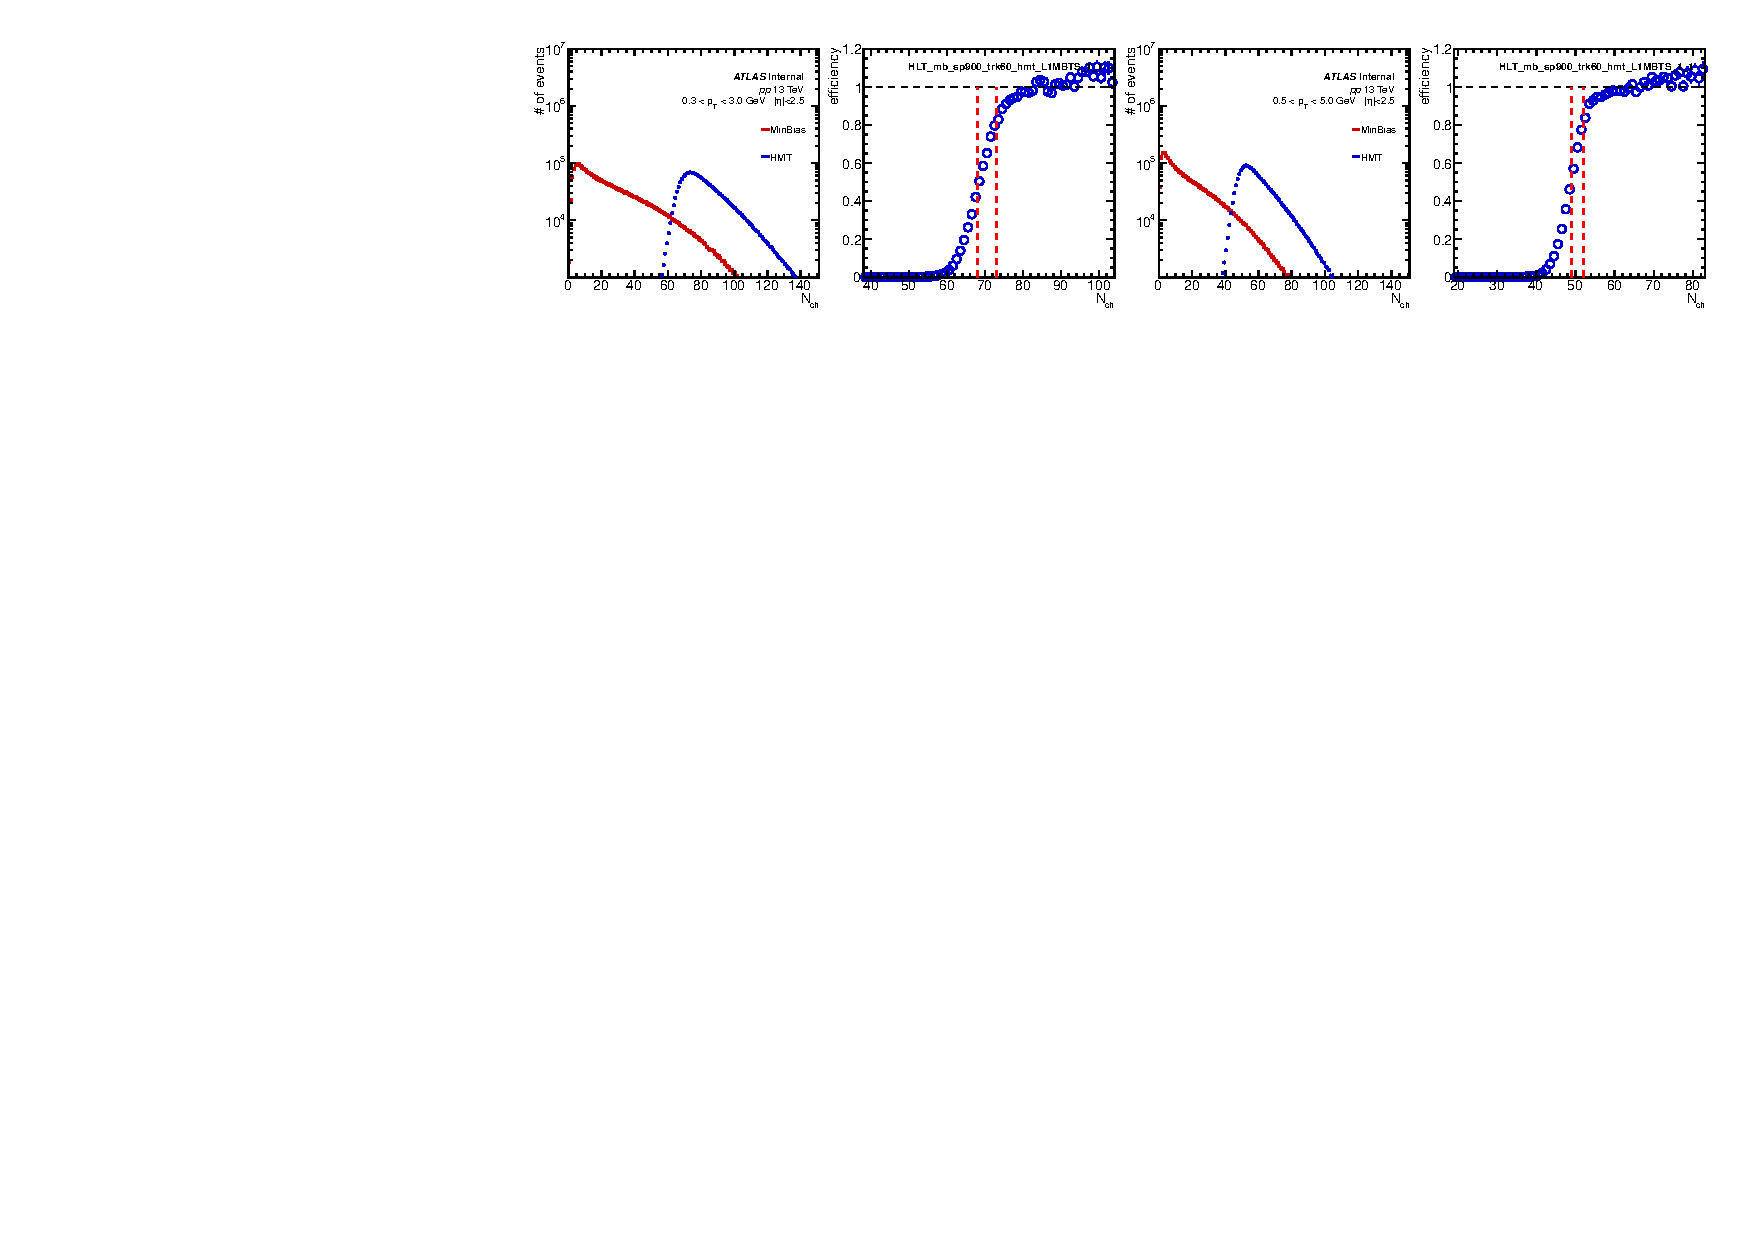
\includegraphics[width=1.\linewidth]{figs/sec_evtSlc/trigEff_pp13_run2/trigEff_Trig19.pdf}
\end{figure}
\begin{figure}[H]
\centering
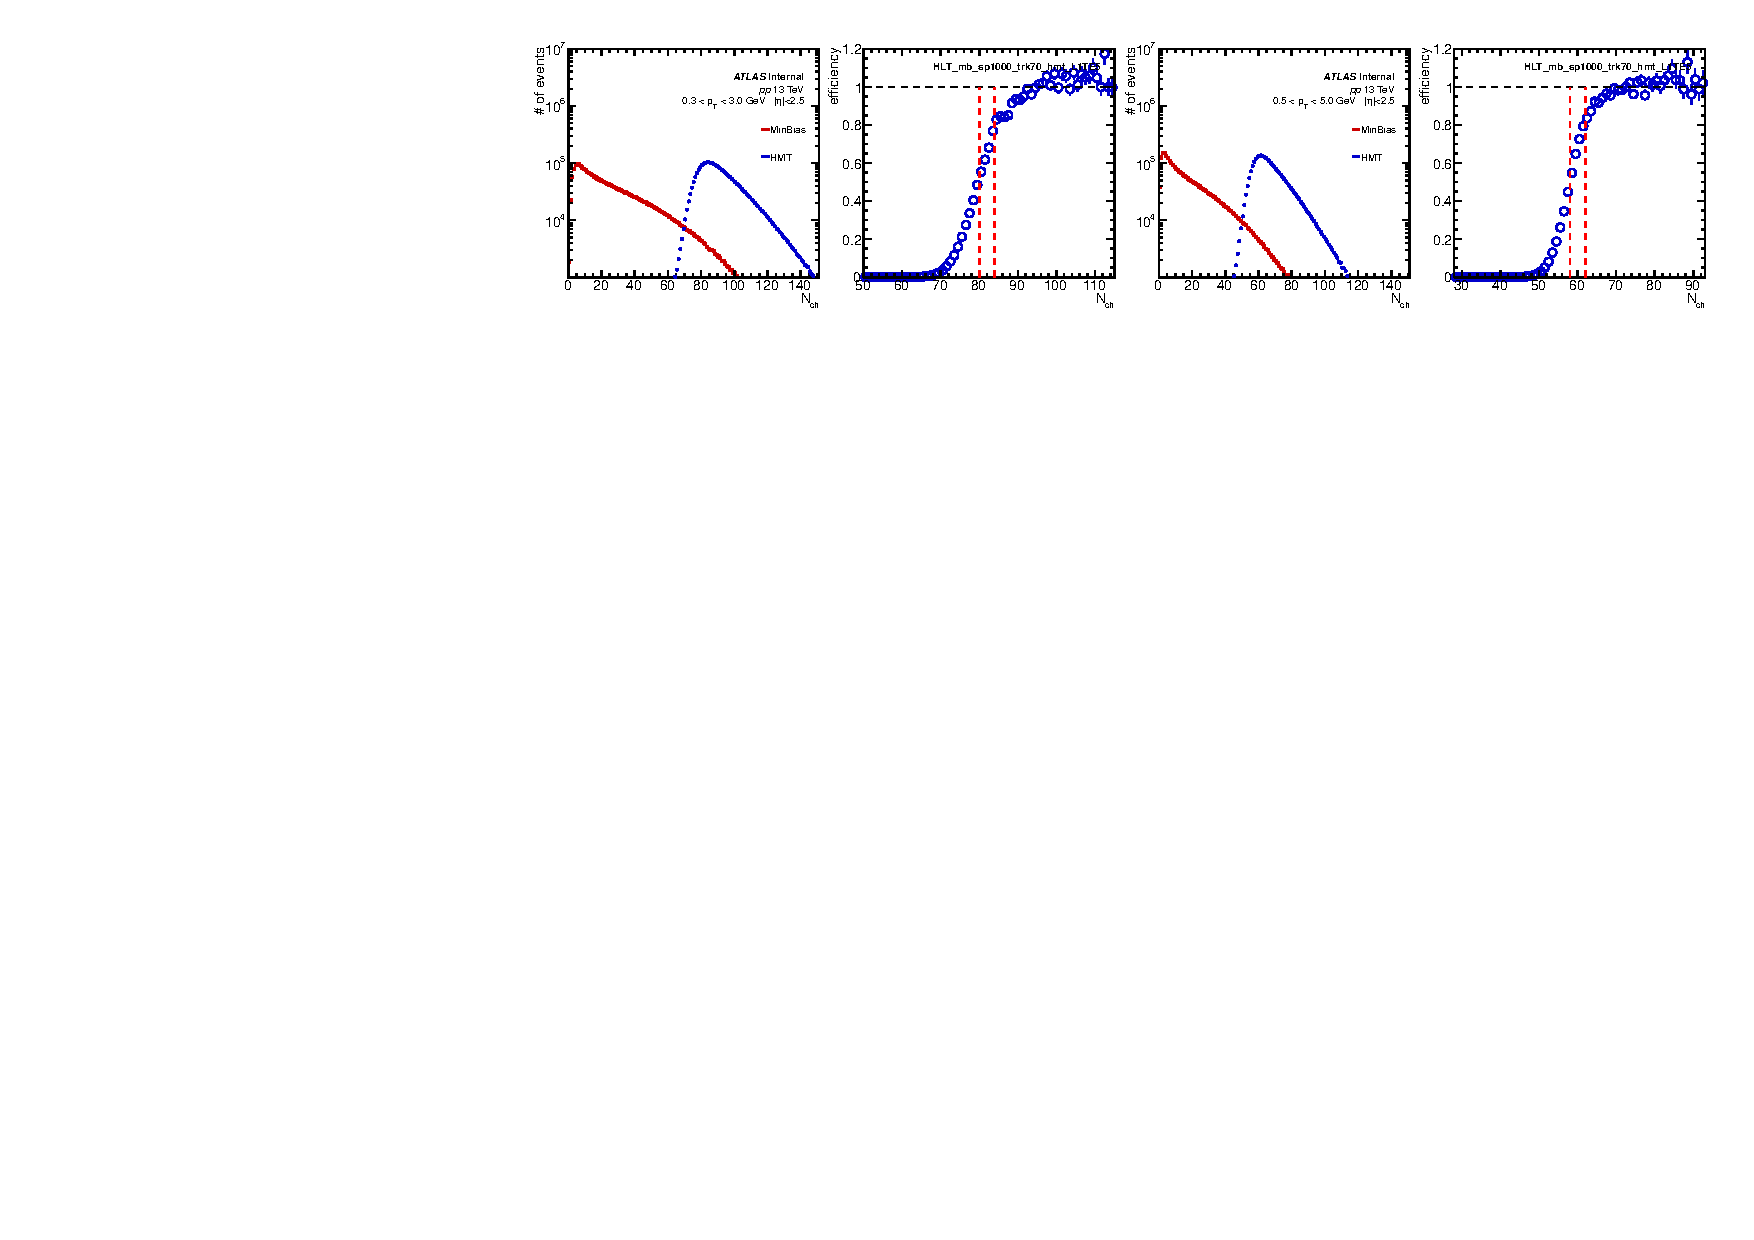
\includegraphics[width=1.\linewidth]{figs/sec_evtSlc/trigEff_pp13_run2/trigEff_Trig22.pdf}
\end{figure}
\begin{figure}[H]
\centering
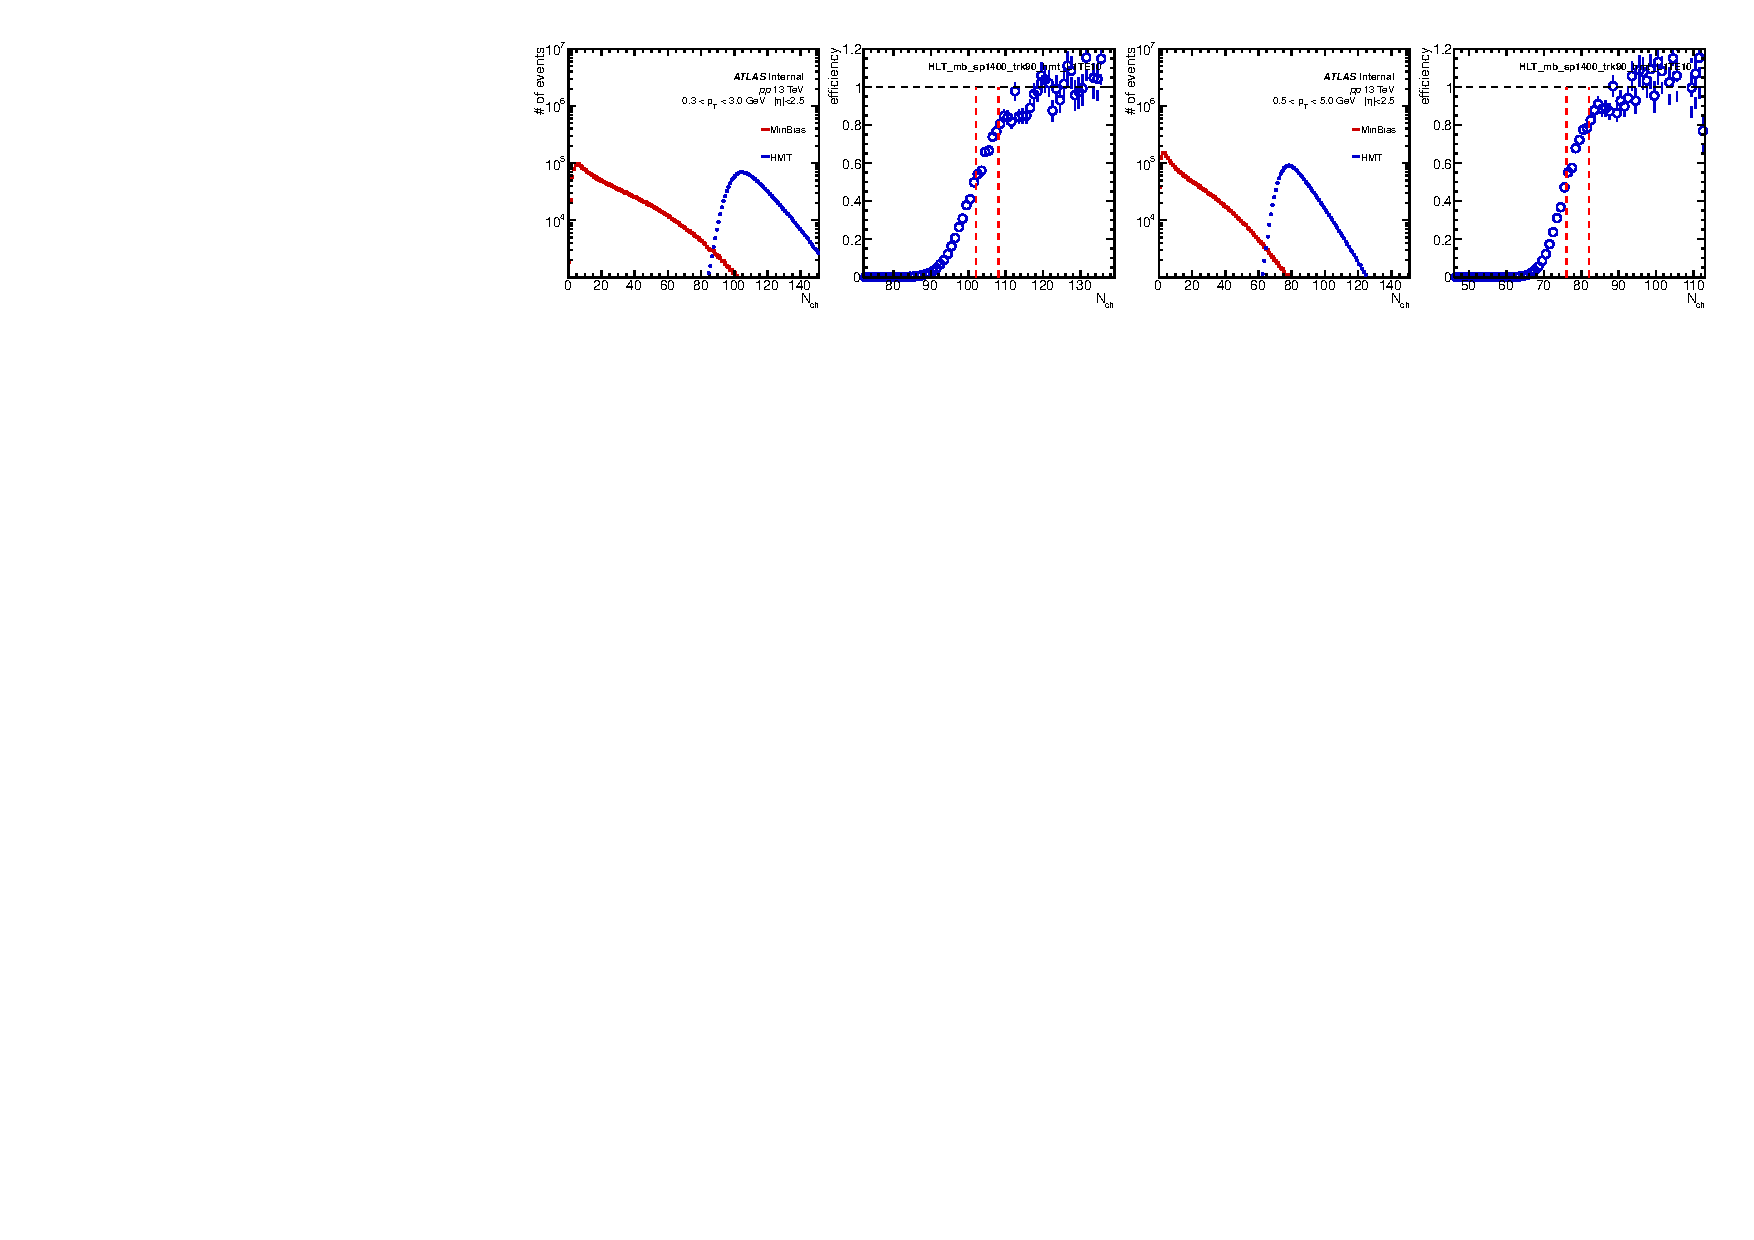
\includegraphics[width=1.\linewidth]{figs/sec_evtSlc/trigEff_pp13_run2/trigEff_Trig24.pdf}
\caption{Trigger efficiencies of all major HMT triggers as a function of number of tracks in two $p_{T}$ ranges: $0.3<p_{T}<3.0$ GeV and $0.5<p_{T}<5.0$ GeV, from 13 TeV $pp$ run period 2. Efficiency is calculated relative to the corresponding MinBias trigger in this run period then scaled to 1.0 in the large $N_{ch}$ region. The two red dash lines indicate 50$\%$ and 80$\%$ efficiency cuts.}
\label{fig:trigEff_pp13_run2}
\end{figure}
Trigger efficiencies of all the major HMT triggers are summarized in Fig.~\ref{fig:trigEff_pp13_run2}, where efficiencies are shown for two $p_{T}$ ranges separately: $0.3<p_{T}<3.0$ GeV and $0.5<p_{T}<5.0$ GeV.



\subsubsection{Run period 3}
The 3rd run period data was taken in 2016 and there is one low-$\mu$ run used for this analysis:
\begin{itemize}

\item Run 305359, peak $\mu=0.06$, 16.5 million events
\begin{itemize}[leftmargin=*]
\item[] \verb|data16_13TeV.00305359.physics_MinBias.recon.AOD.r8489/|
\end{itemize}

\end{itemize}
The major MinBias and HMT triggers applied in this run period are:
\begin{itemize}
\item \verb|HLT_mb_mbts_L1MBTS_1_1|
\item \verb|HLT_noalg_mb_L1TE30|
\item \verb|HLT_mb_sp700_hmtperf_L1TE5|
\item \verb|HLT_mb_sp1500_hmtperf_L1TE10|
\item \verb|HLT_mb_sp1000_trk70_hmt_L1TE5|
\item \verb|HLT_mb_sp1400_trk90_hmt_L1TE10|
\end{itemize}

\begin{figure}[H]
\centering
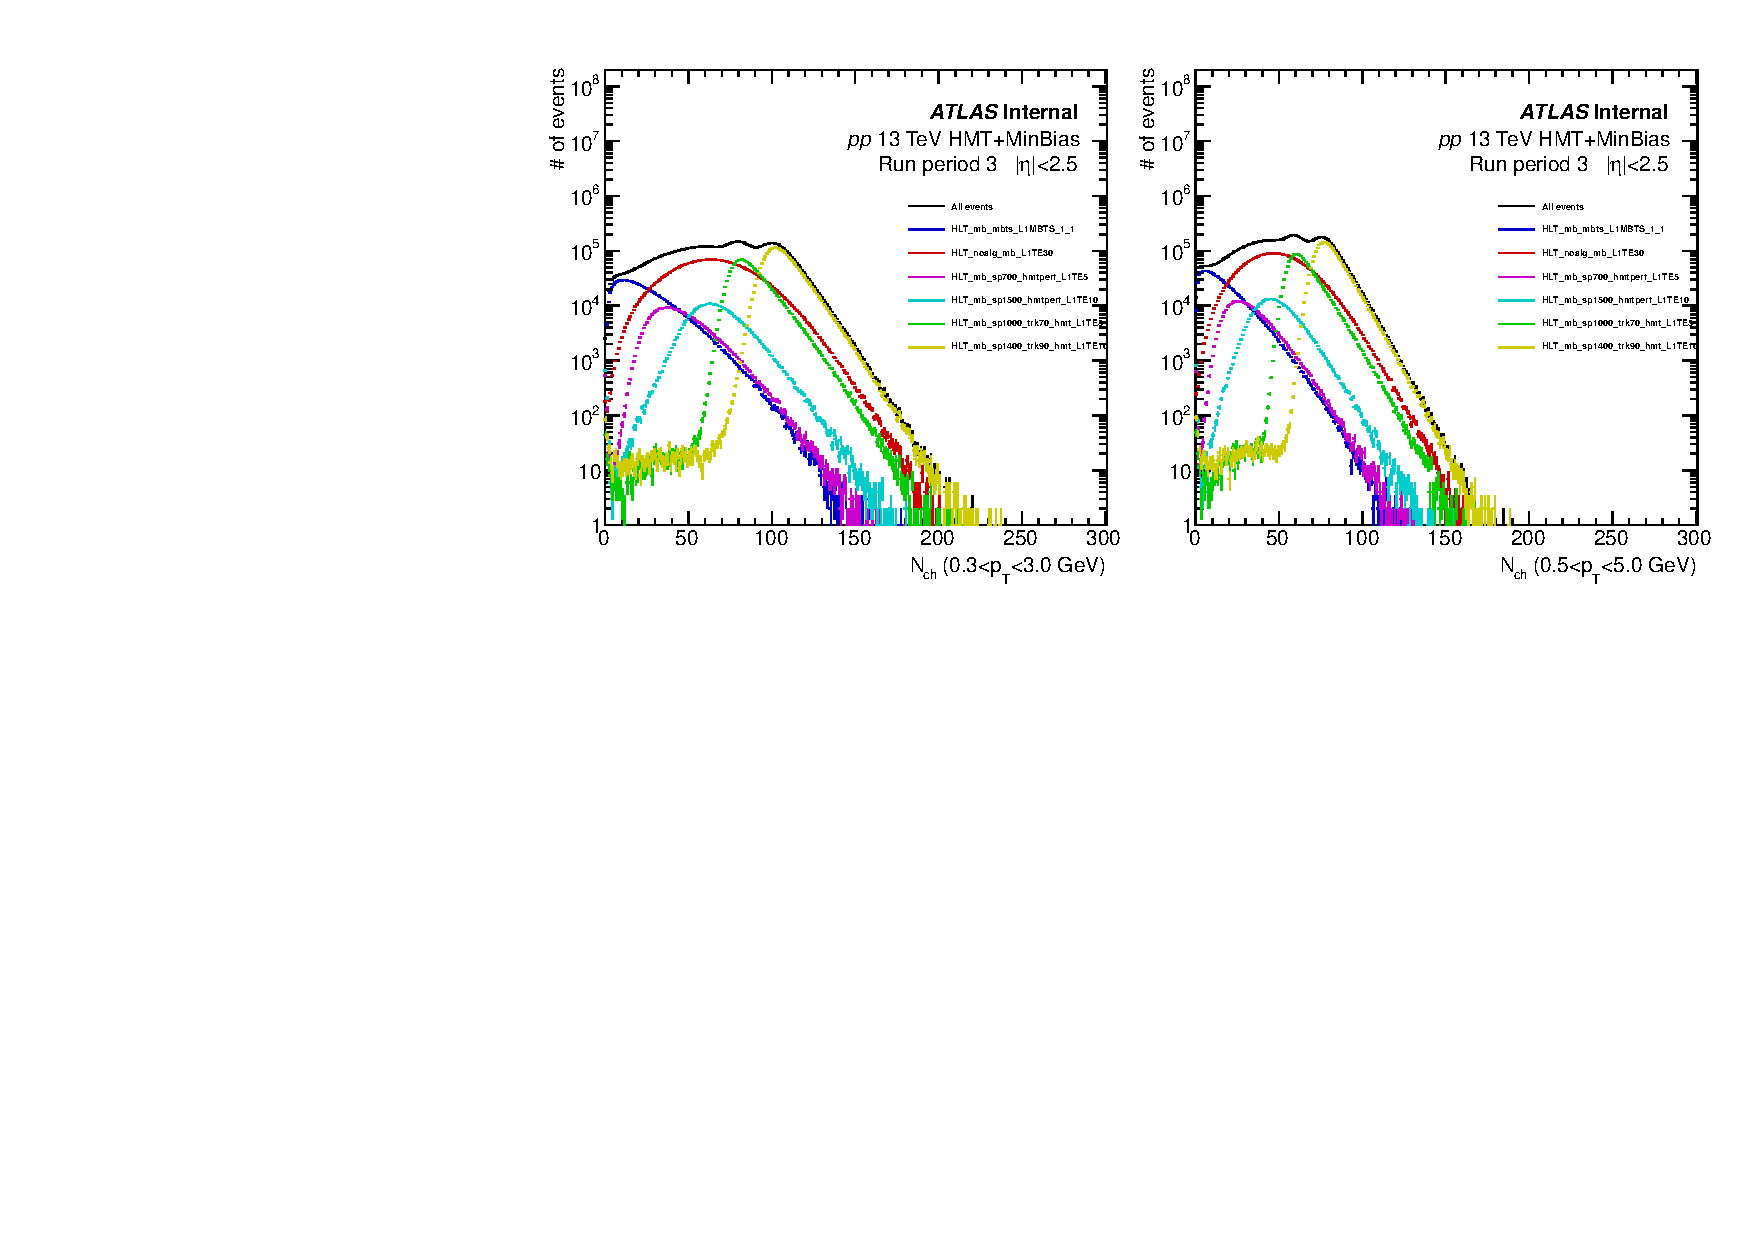
\includegraphics[width=.9\linewidth]{figs/sec_evtSlc/trkDis_pp13_run3.pdf}
\caption{Distribution of number of tracks with two $p_{T}$ thresholds: $0.3<p_{T}<3.0$ GeV and $0.5<p_{T}<5.0$ GeV, in 13 TeV $pp$ run period 3. The major MinBias and HMT triggers are plotted separately.}
\label{fig:trkDis_pp13_run3}
\end{figure}
The summary of statistics with all the major triggers used in this analysis are shown in Fig.~\ref{fig:trkDis_pp13_run3}.

\begin{figure}[H]
\centering
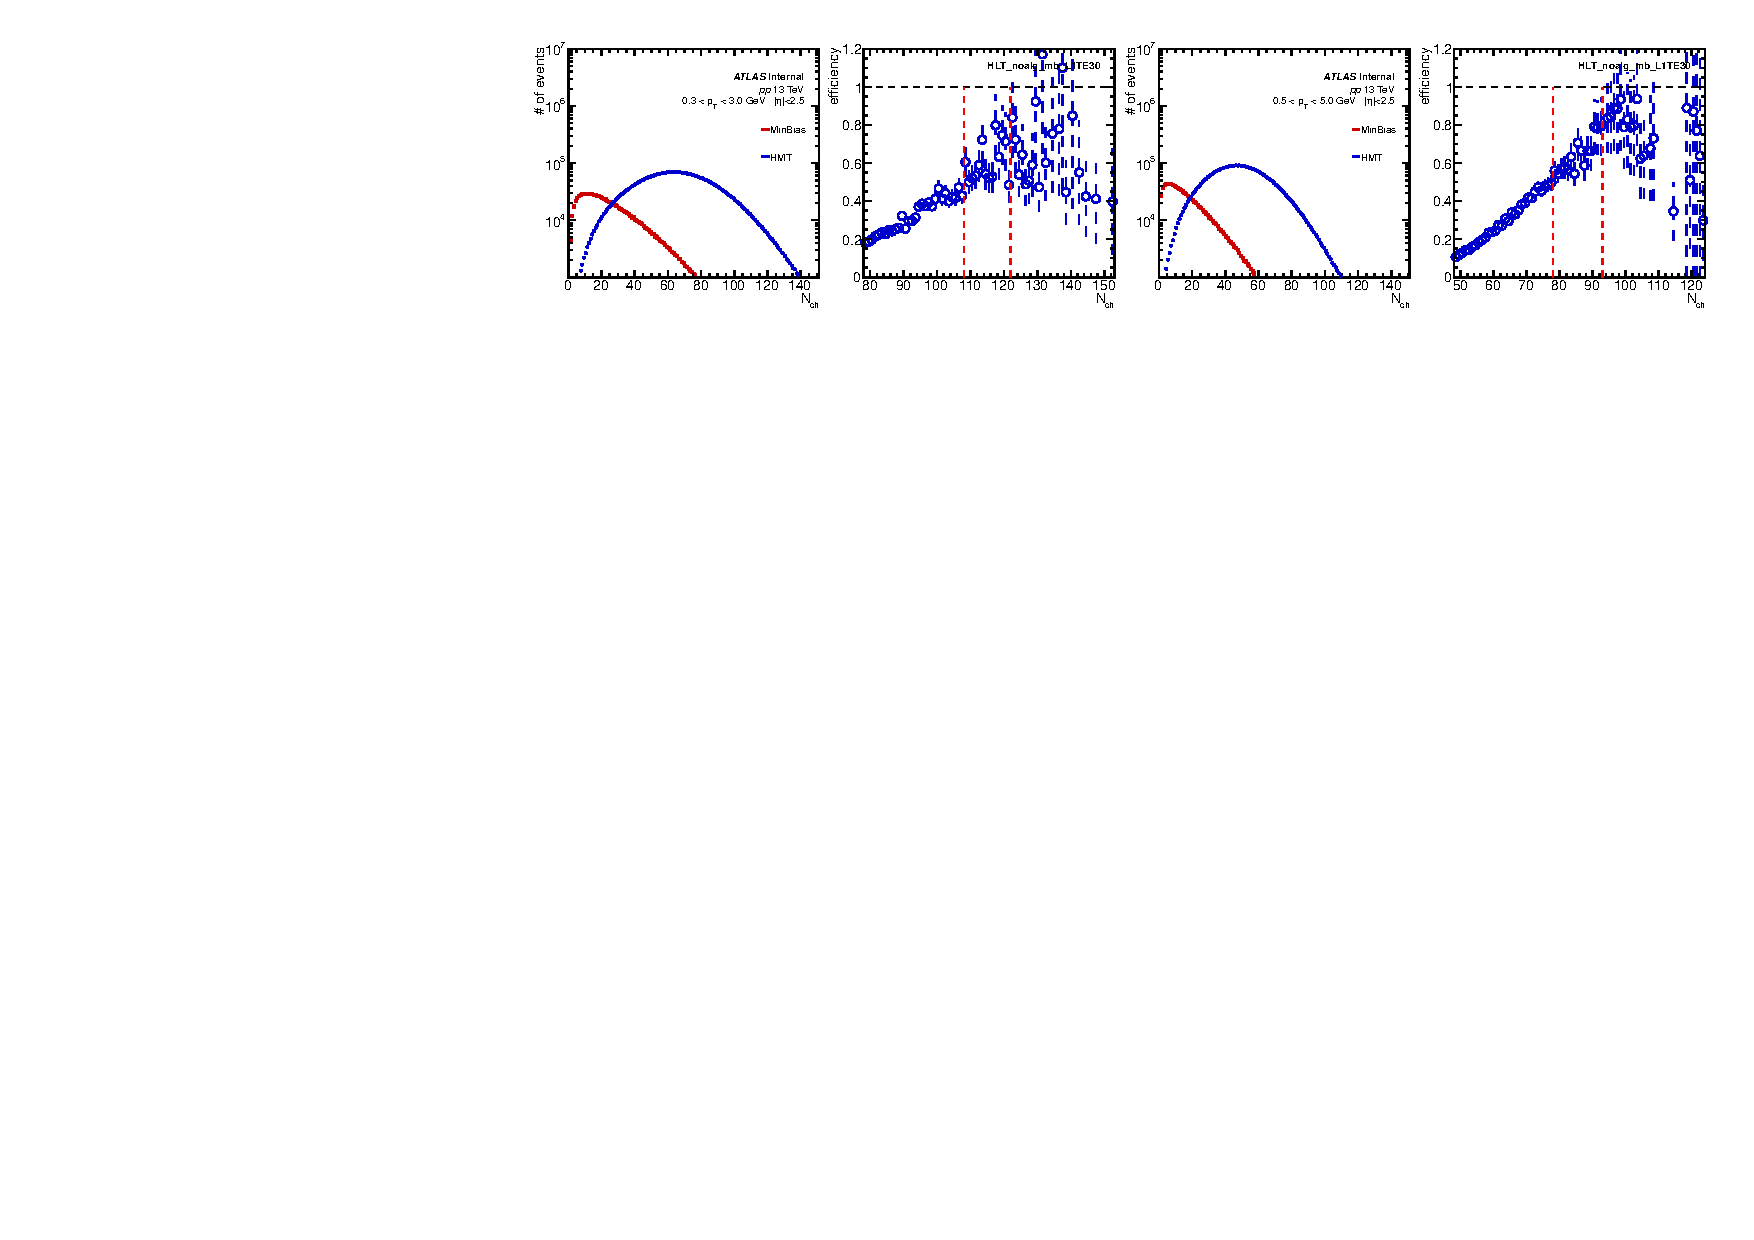
\includegraphics[width=1.\linewidth]{figs/sec_evtSlc/trigEff_pp13_run3/trigEff_Trig2.pdf}
\end{figure}
\begin{figure}[H]
\centering
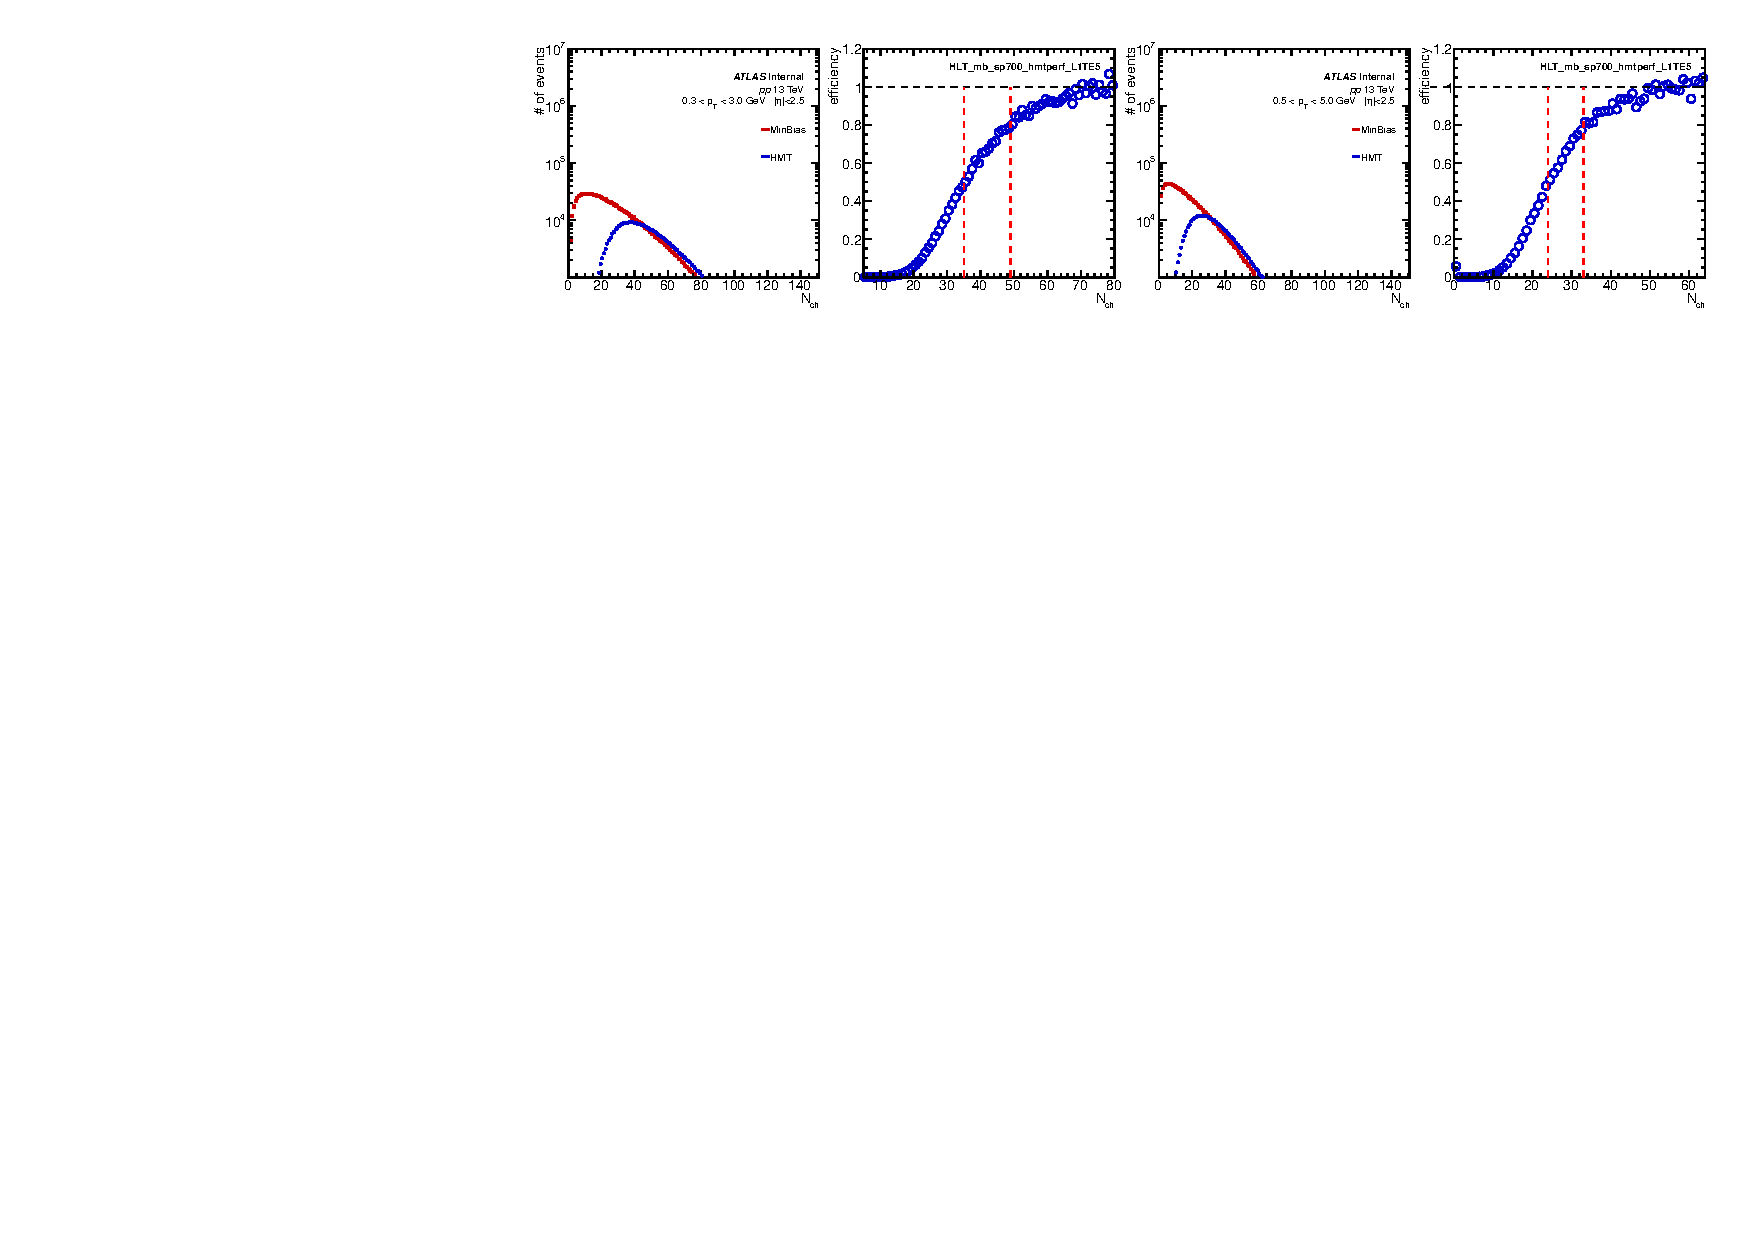
\includegraphics[width=1.\linewidth]{figs/sec_evtSlc/trigEff_pp13_run3/trigEff_Trig6.pdf}
\end{figure}
\begin{figure}[H]
\centering
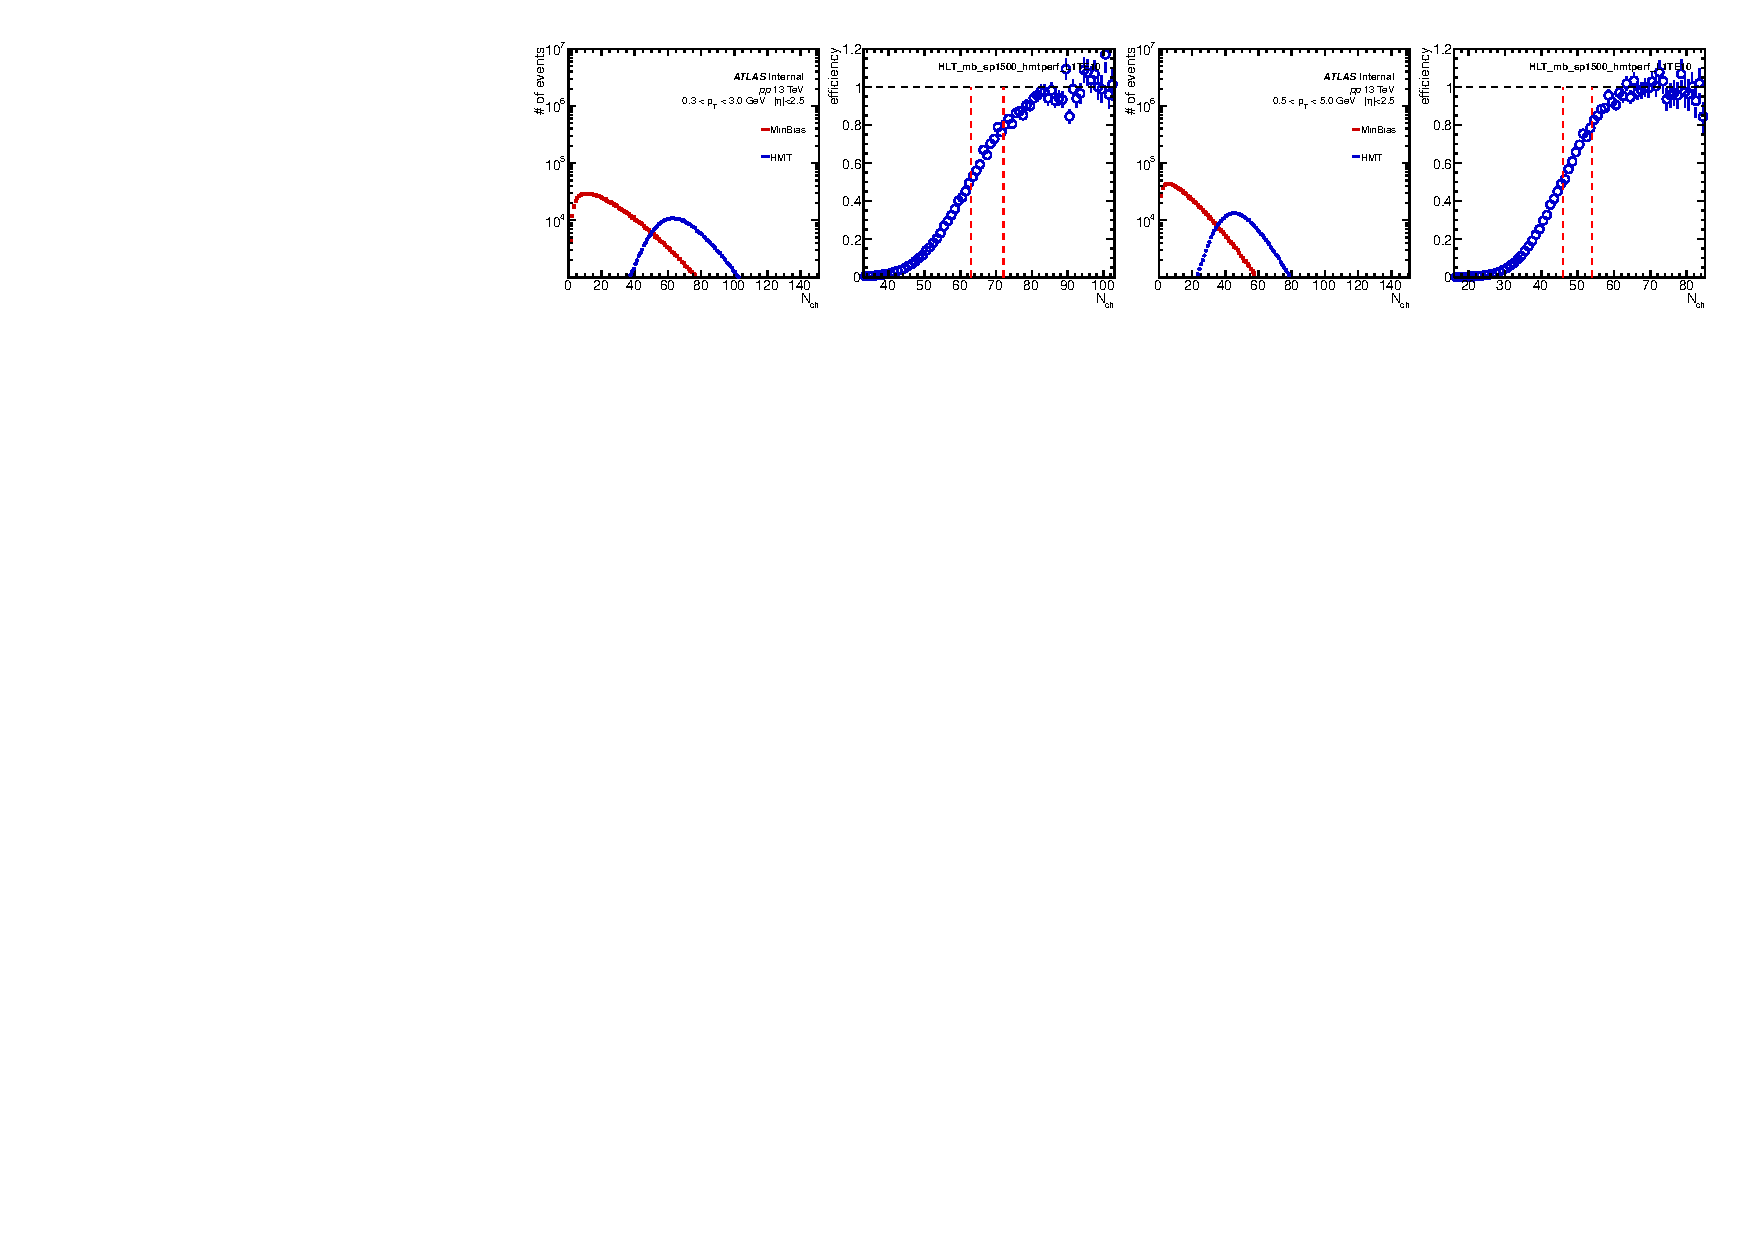
\includegraphics[width=1.\linewidth]{figs/sec_evtSlc/trigEff_pp13_run3/trigEff_Trig7.pdf}
\end{figure}
\begin{figure}[H]
\centering
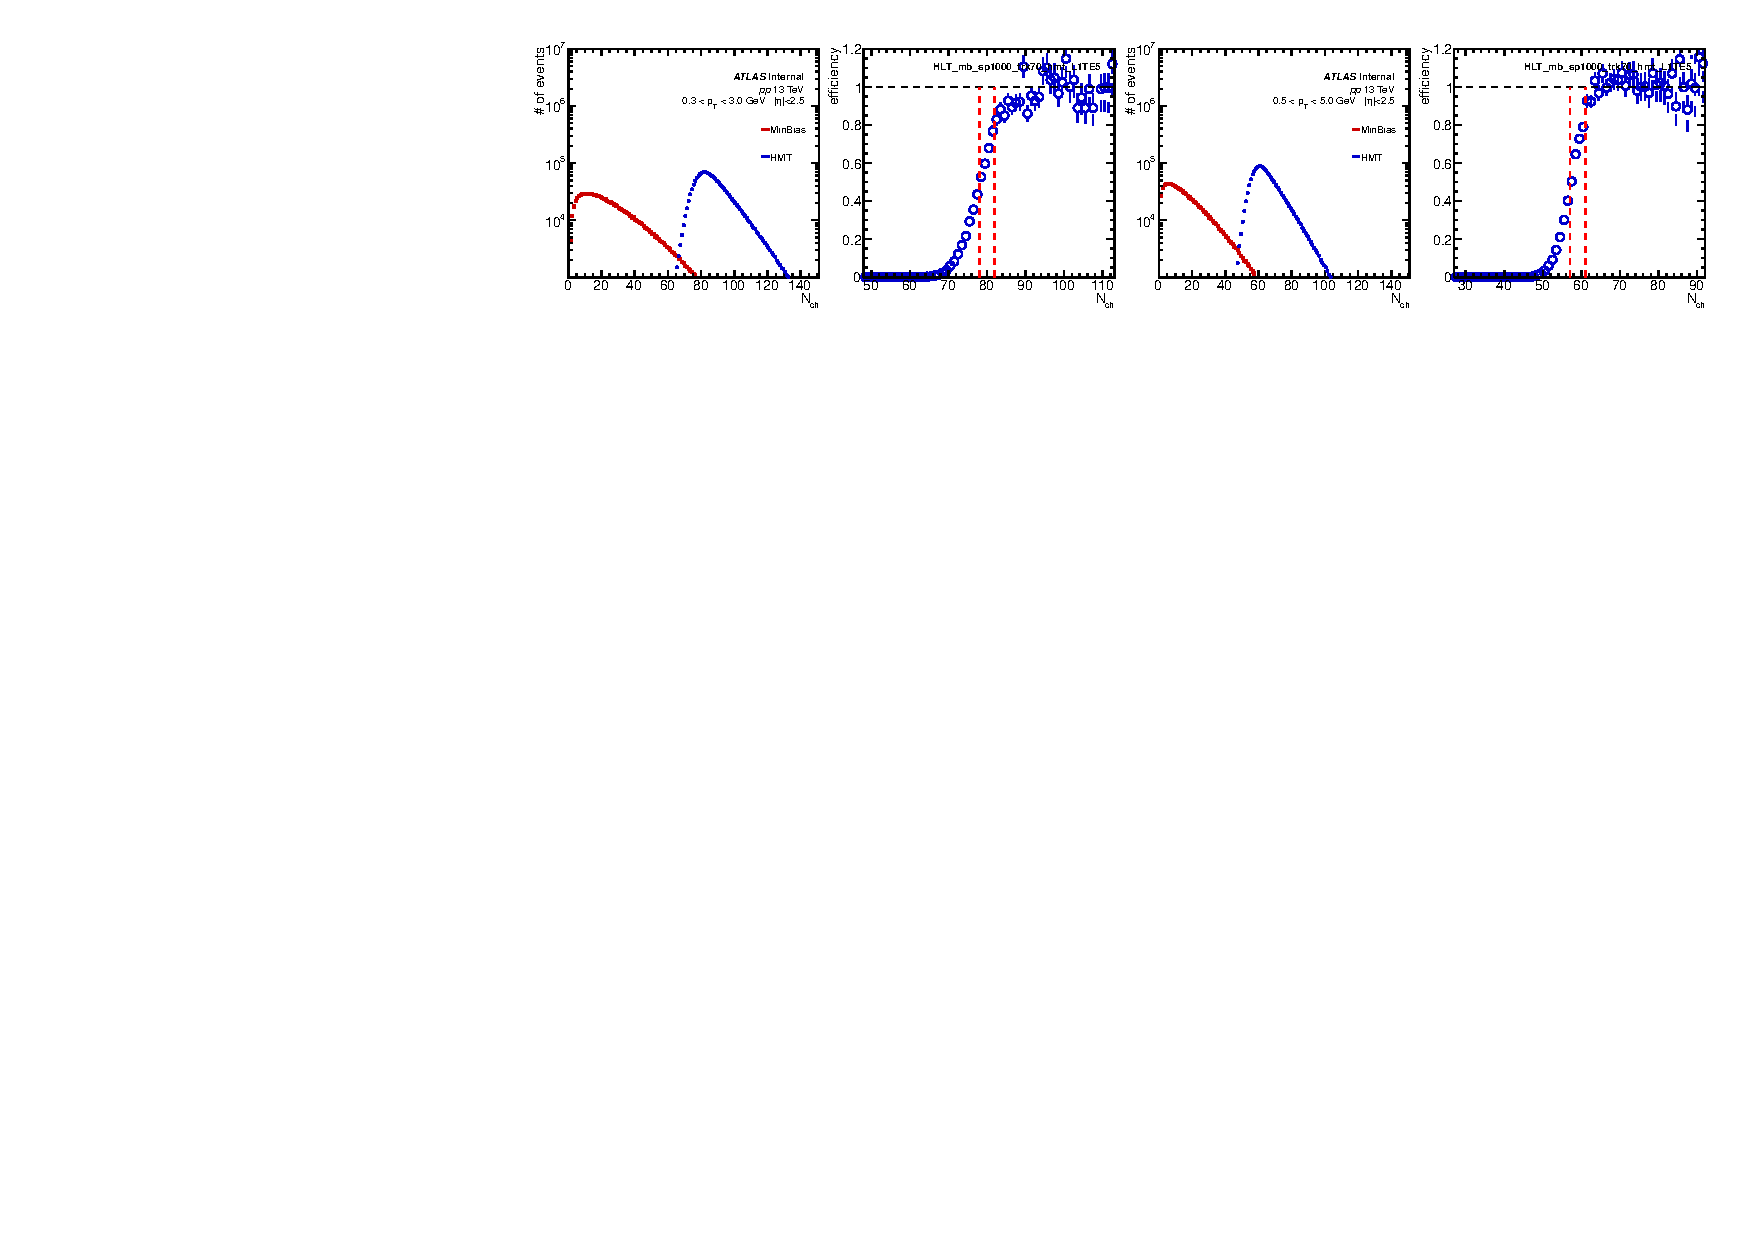
\includegraphics[width=1.\linewidth]{figs/sec_evtSlc/trigEff_pp13_run3/trigEff_Trig9.pdf}
\end{figure}
\begin{figure}[H]
\centering
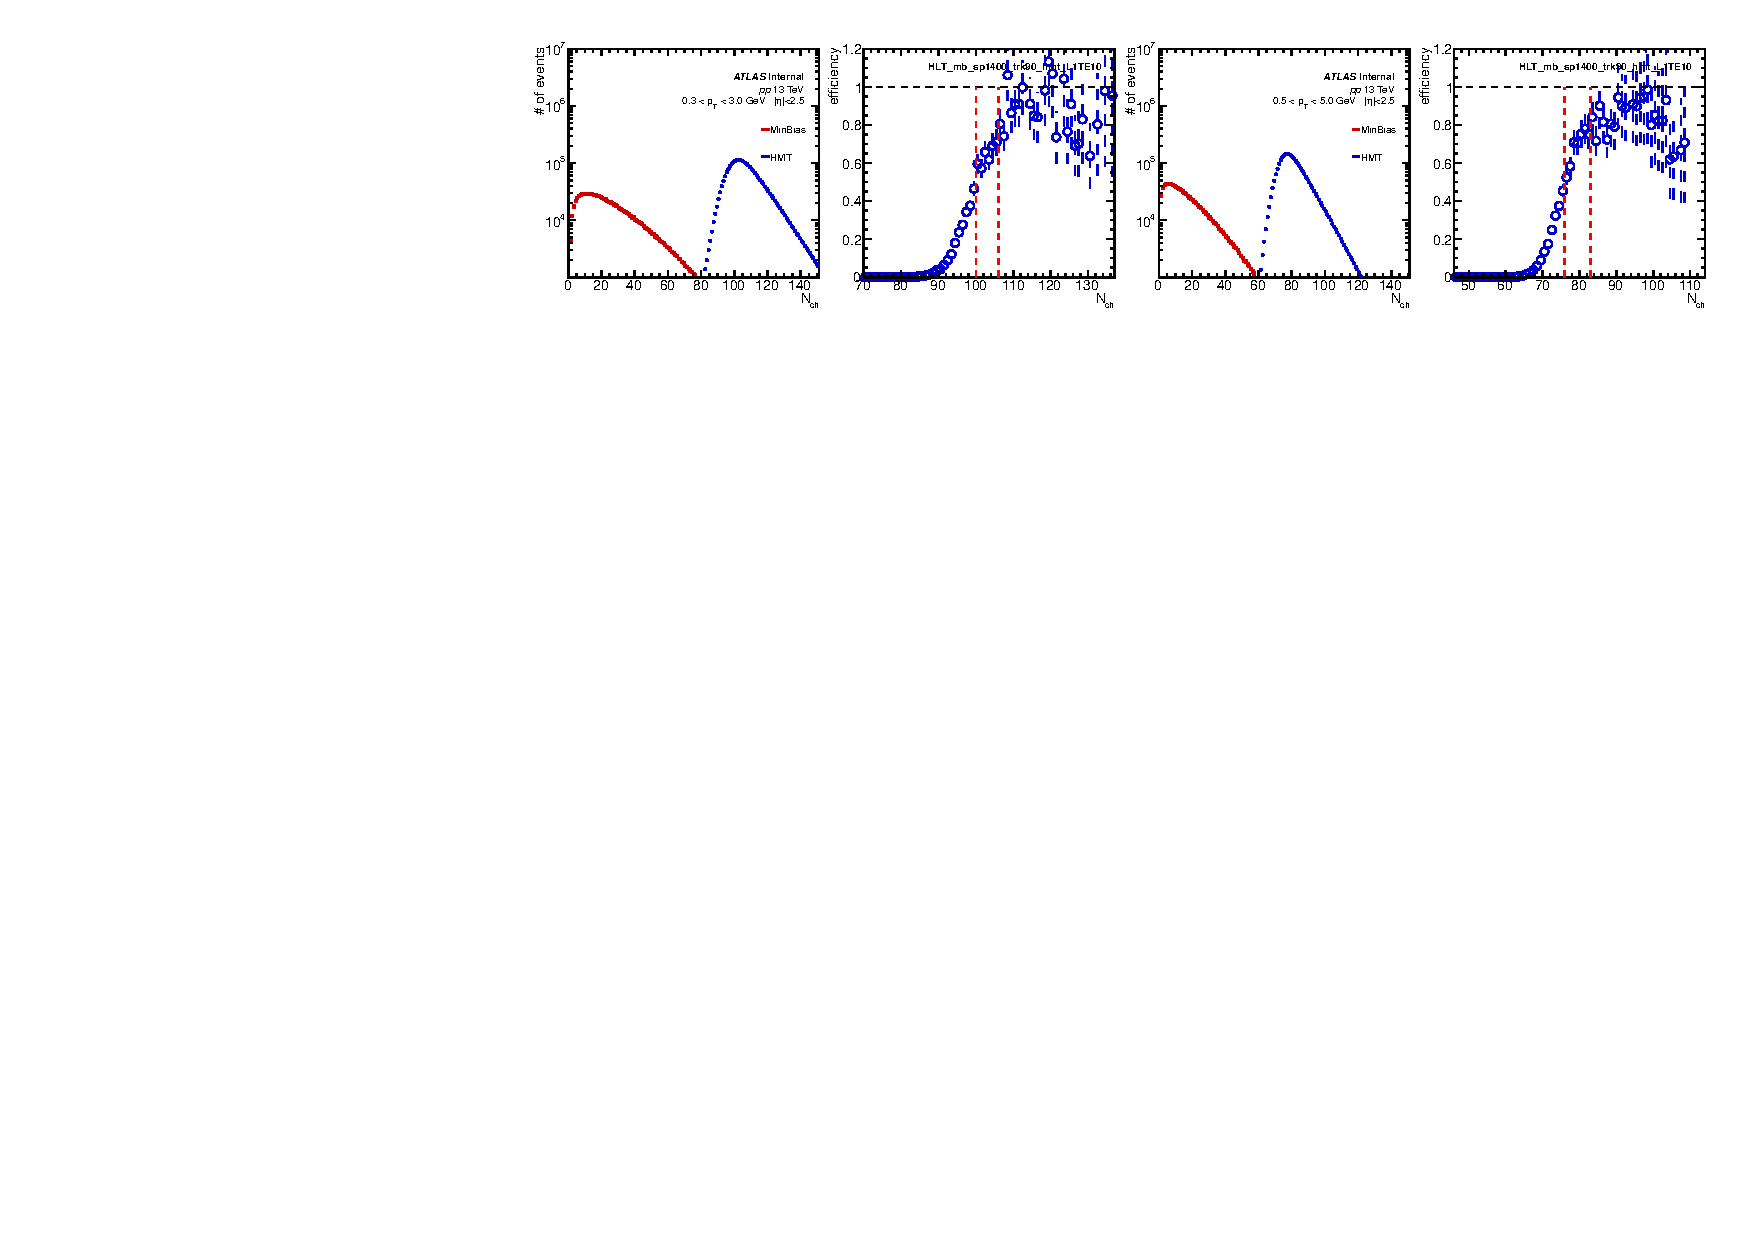
\includegraphics[width=1.\linewidth]{figs/sec_evtSlc/trigEff_pp13_run3/trigEff_Trig11.pdf}
\caption{Trigger efficiencies of all major HMT triggers as a function of number of tracks in two $p_{T}$ ranges: $0.3<p_{T}<3.0$ GeV and $0.5<p_{T}<5.0$ GeV, from 13 TeV $pp$ run period 3. Efficiency is calculated relative to the corresponding MinBias trigger in this run period then scaled to 1.0 in the large $N_{ch}$ region. The two red dash lines indicate 50$\%$ and 80$\%$ efficiency cuts.}
\label{fig:trigEff_pp13_run3}
\end{figure}
Trigger efficiencies of all the major HMT triggers are summarized in Fig.~\ref{fig:trigEff_pp13_run3}, where efficiencies are shown for two $p_{T}$ ranges separately: $0.3<p_{T}<3.0$ GeV and $0.5<p_{T}<5.0$ GeV.



\subsubsection{Run period 4}
The 4th run period data was taken in 2016 and there are 3 intermediate-$\mu$ runs used for this analysis:
\begin{itemize}

\item Run 309314, peak $\mu=0.36$, 13.2 million events
\begin{itemize}[leftmargin=*]
\item[] \verb|data16_13TeV.00309314.physics_MinBias.recon.AOD.r8576/|
\end{itemize}

\item Run 309346, peak $\mu=0.33$, 7.5 million events
\begin{itemize}[leftmargin=*]
\item[] \verb|data16_13TeV.00309346.physics_MinBias.recon.AOD.r8576/|
\end{itemize}

\item Run 310216, peak $\mu=0.31$, 79.9 million events
\begin{itemize}[leftmargin=*]
\item[] \verb|data16_13TeV.00310216.physics_MinBias.recon.AOD.r8600/|
\end{itemize}

\end{itemize}
The major MinBias and HMT triggers applied in this run period are:
\begin{itemize}
\item \verb|HLT_mb_sptrk|
\item \verb|HLT_mb_sp900_trk50_hmt_L1TE5|
\item \verb|HLT_mb_sp1000_trk70_hmt_L1TE10.0ETA24|
\item \verb|HLT_mb_sp1400_trk90_hmt_L1TE20.0ETA24|
\end{itemize}
where a new trigger item has been introduced:
\begin{itemize}
\item \verb|L1TEX.0ETA24|: L1 trigger is seeded at L1 total energy from the restricted $\eta$ range: $-2.4<\eta<2.4$ and the threshold is X GeV;
\end{itemize}

\begin{figure}[H]
\centering
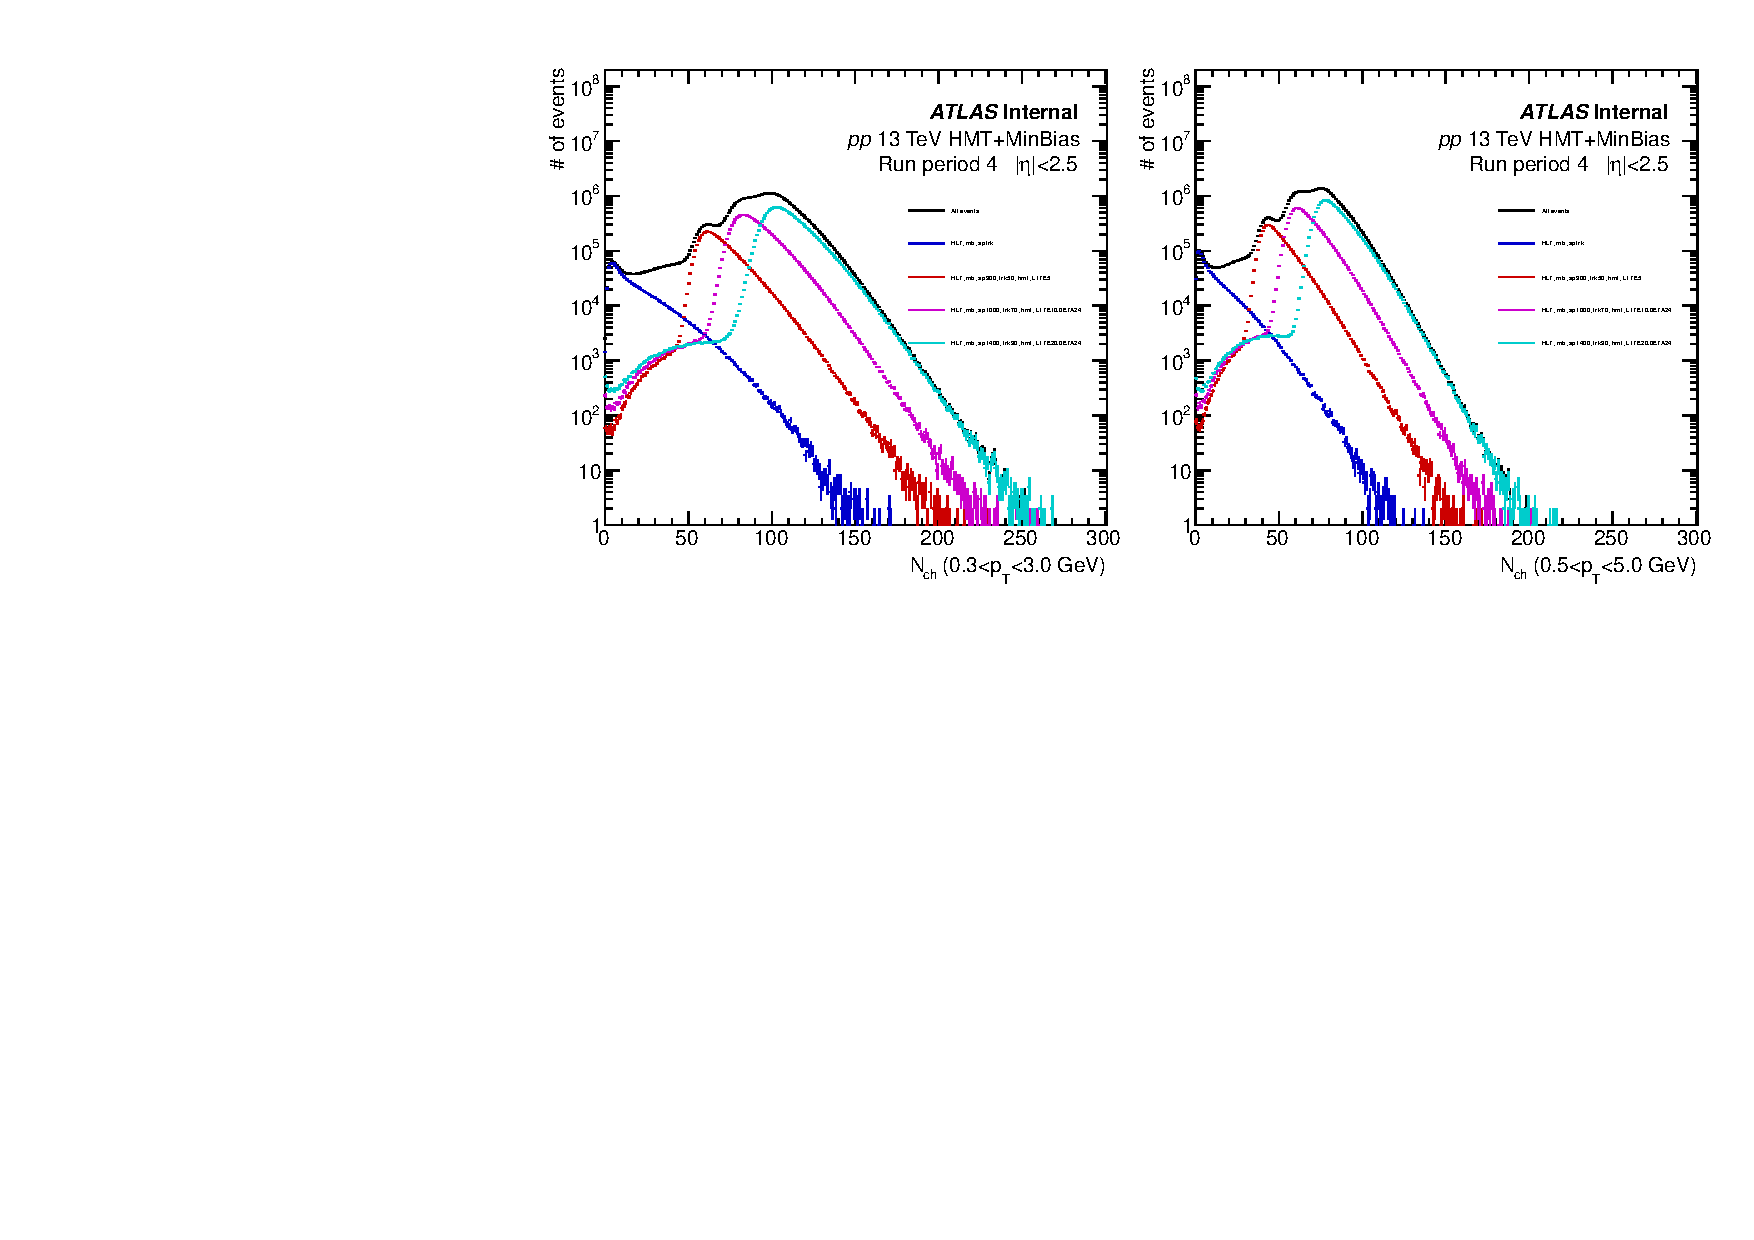
\includegraphics[width=.9\linewidth]{figs/sec_evtSlc/trkDis_pp13_run4.pdf}
\caption{Distribution of number of tracks with two $p_{T}$ thresholds: $0.3<p_{T}<3.0$ GeV and $0.5<p_{T}<5.0$ GeV, in 13 TeV $pp$ run period 4. The major MinBias and HMT triggers are plotted separately.}
\label{fig:trkDis_pp13_run4}
\end{figure}
The summary of statistics with all the major triggers used in this analysis are shown in Fig.~\ref{fig:trkDis_pp13_run4}.

\begin{figure}[H]
\centering
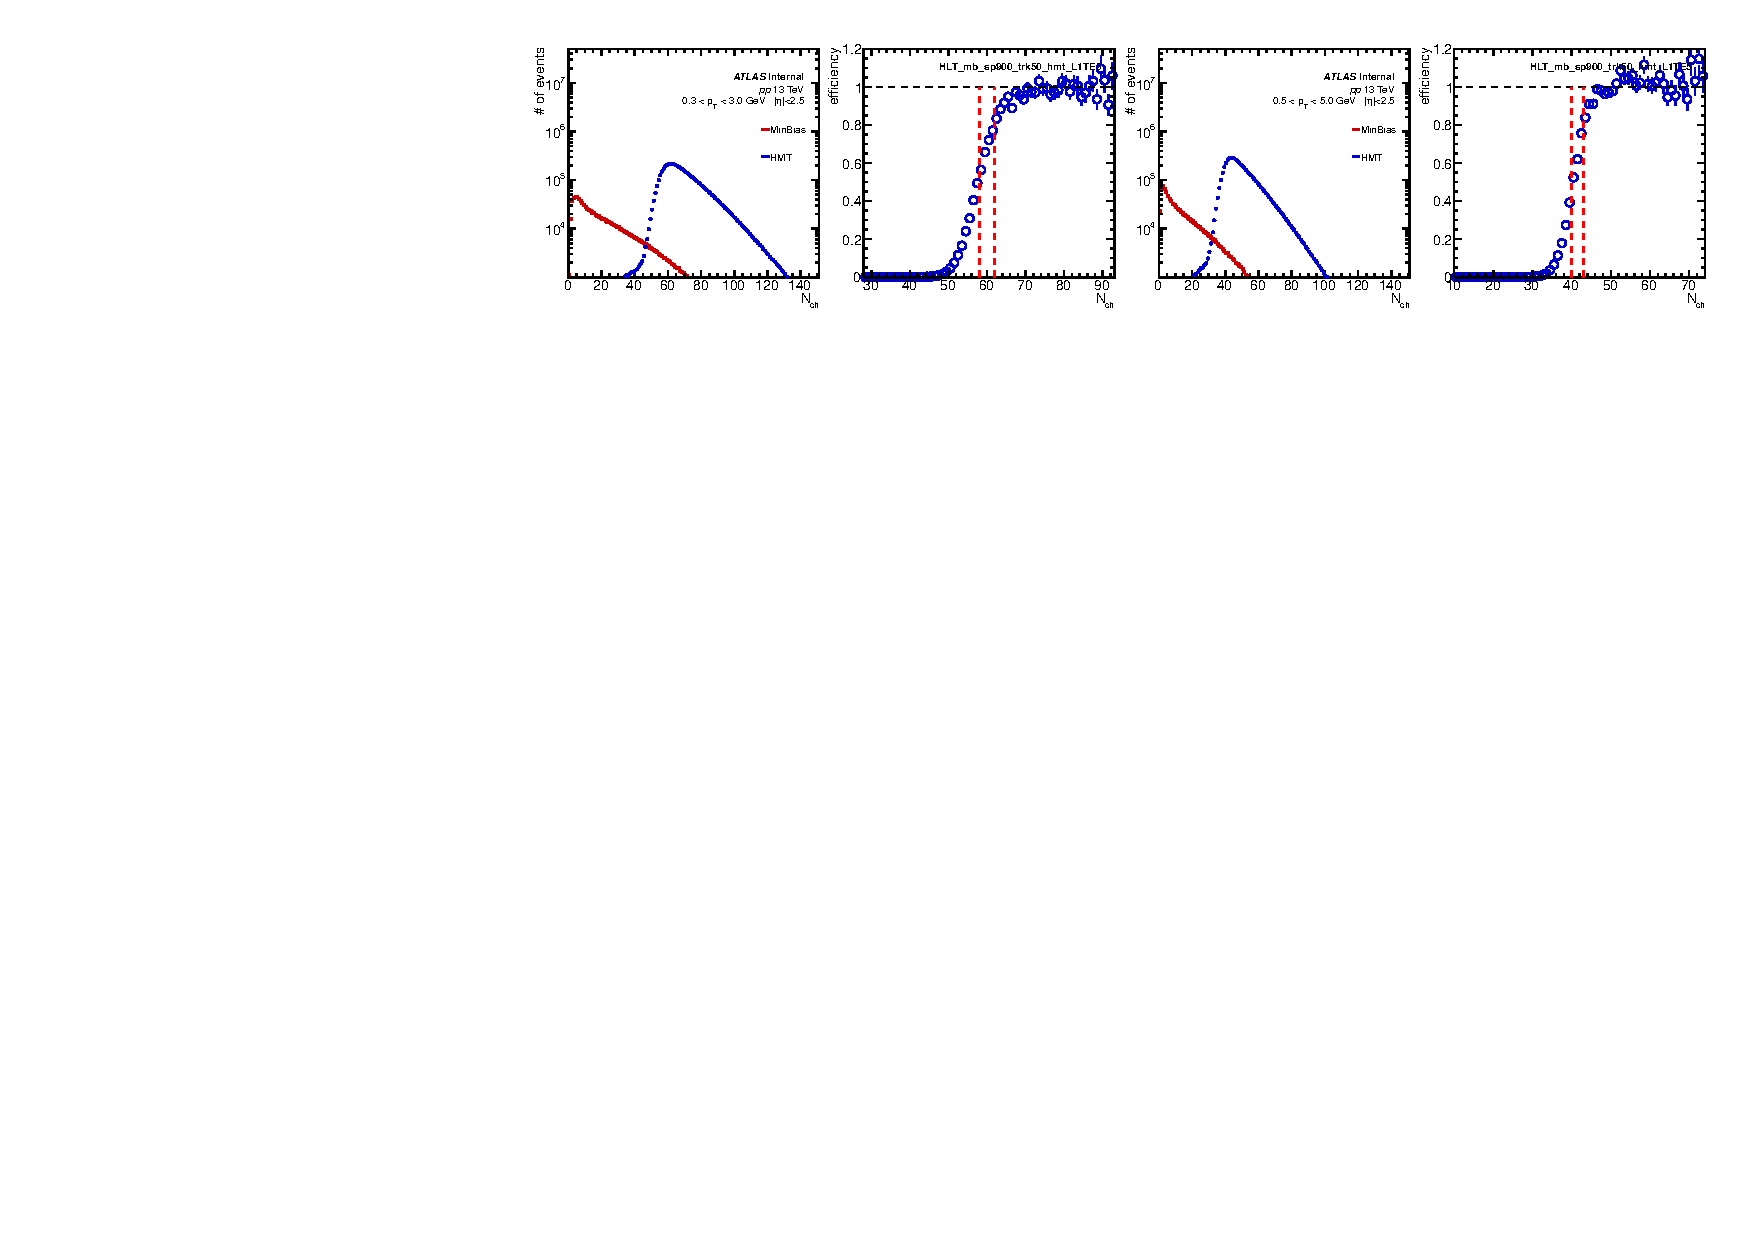
\includegraphics[width=1.\linewidth]{figs/sec_evtSlc/trigEff_pp13_run4/trigEff_Trig18.pdf}
\end{figure}
\begin{figure}[H]
\centering
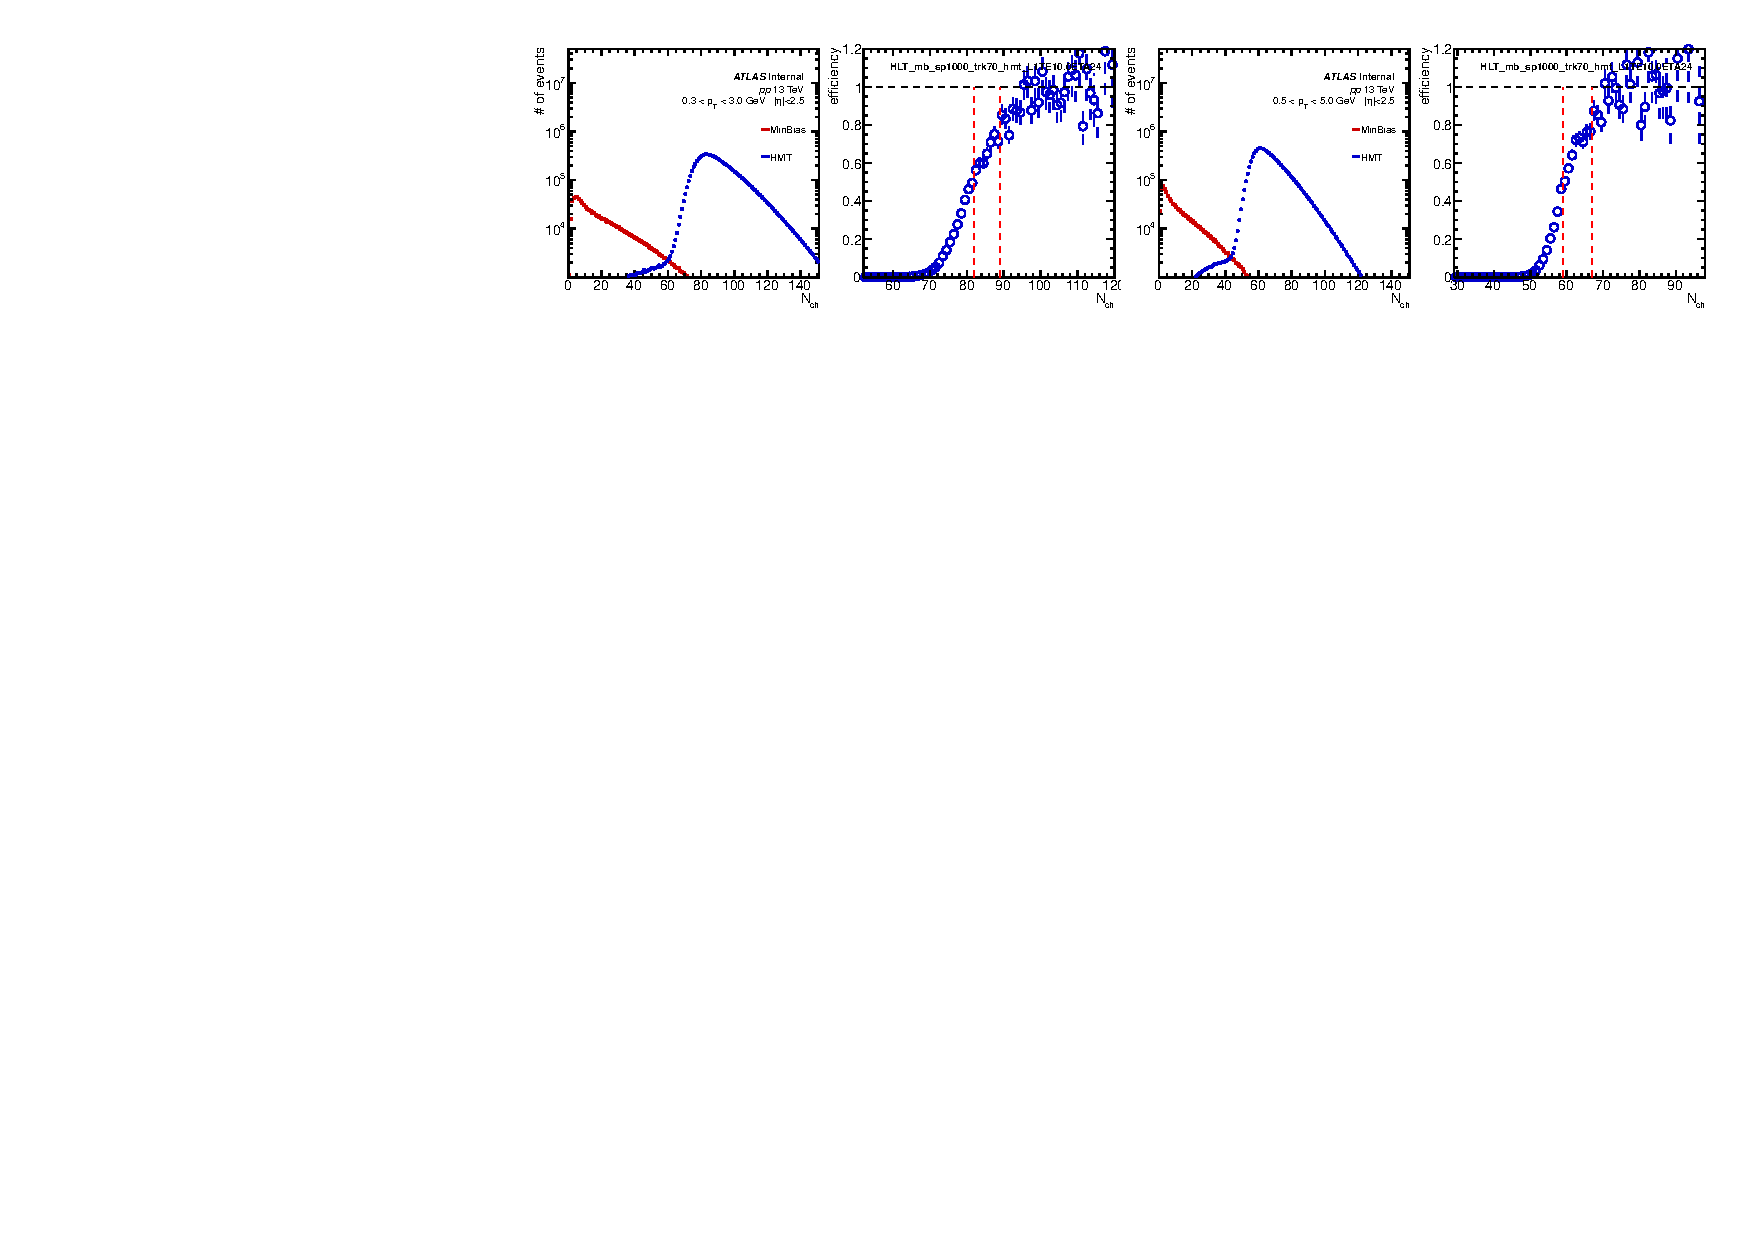
\includegraphics[width=1.\linewidth]{figs/sec_evtSlc/trigEff_pp13_run4/trigEff_Trig24.pdf}
\end{figure}
\begin{figure}[H]
\centering
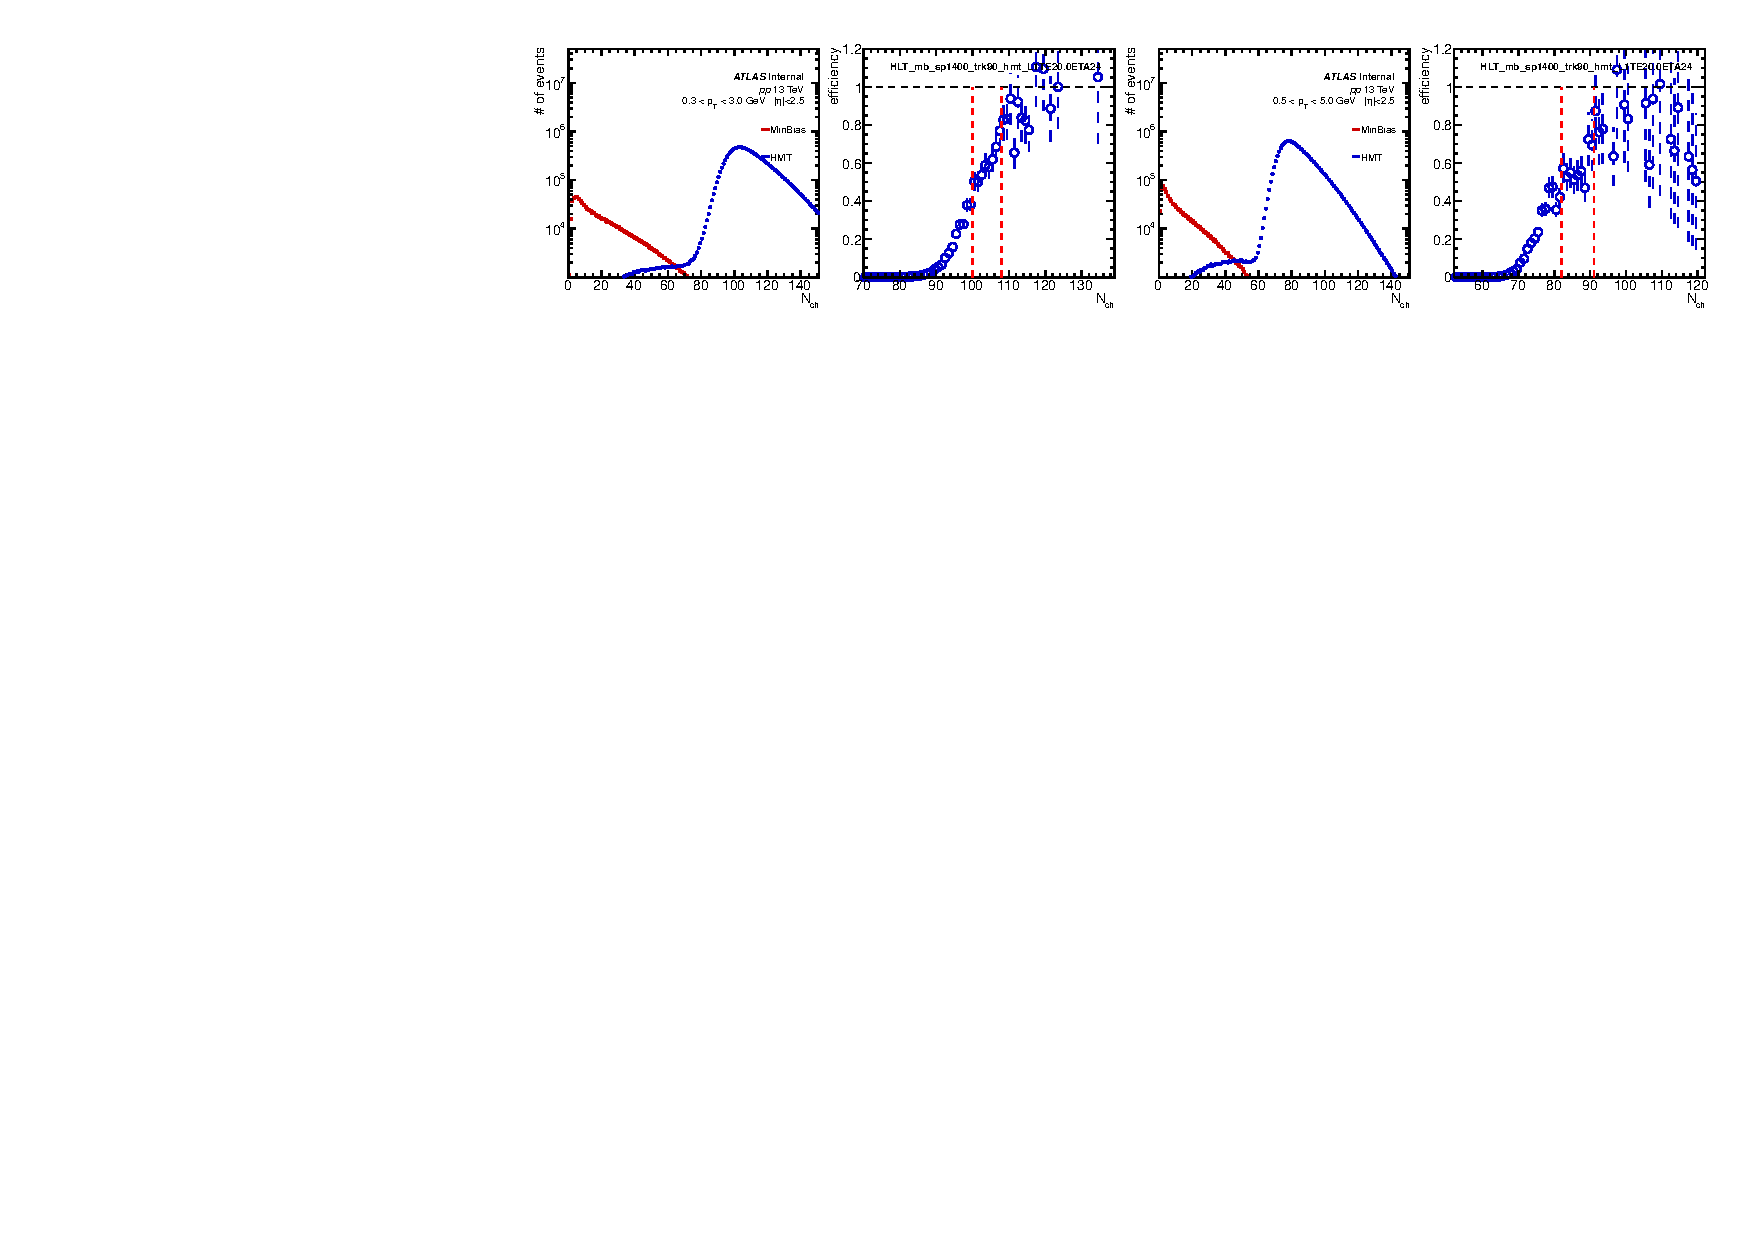
\includegraphics[width=1.\linewidth]{figs/sec_evtSlc/trigEff_pp13_run4/trigEff_Trig30.pdf}
\caption{Trigger efficiencies of all major HMT triggers as a function of number of tracks in two $p_{T}$ ranges: $0.3<p_{T}<3.0$ GeV and $0.5<p_{T}<5.0$ GeV, from 13 TeV $pp$ run period 4. Efficiency is calculated relative to the corresponding MinBias trigger in this run period then scaled to 1.0 in the large $N_{ch}$ region. The two red dash lines indicate 50$\%$ and 80$\%$ efficiency cuts.}
\label{fig:trigEff_pp13_run4}
\end{figure}
Trigger efficiencies of all the major HMT triggers are summarized in Fig.~\ref{fig:trigEff_pp13_run4}, where efficiencies are shown for two $p_{T}$ ranges separately: $0.3<p_{T}<3.0$ GeV and $0.5<p_{T}<5.0$ GeV.



\subsubsection{PYTHIA for $pp$ 13 TeV data}

The tracking efficiency applied in this analysis were identical to the ATLAS previous cumulant measurement \verb|ATL-COM-PHYS-2015-740|. The following studies are independent to the other analysis team, and the final results of $c_{2}{4}$ are checked to be consistent no matter which tracking efficiency map is applied.

The PYTHIA~\cite{Sjostrand:2007gs} A2 tune~\cite{atlas:6} was used to produce $pp$ collisions with the same energy as in the data. The detector response is simulated with GEANT 4 with conditions matching those present during the data-taking. The simulated events are reconstructed with the same algorithms as data, in particular using the same track reconstruction as for the data.

The list of PYTHIA samples is shown in the following:
\begin{itemize}
\item 20 million ND sample
\begin{itemize}[leftmargin=*]
\item[] \verb|mc15_13TeV.361203.Pythia8_A2_MSTW2008LO_ND_minbias.merge.AOD.|
\item[] \verb|e3639_a782_a787_r6264/|
\end{itemize}
\item 1 million HMT sample with $N_{ch}>120$
\begin{itemize}[leftmargin=*]
\item[] \verb|mc15_13TeV.361214.Pythia8_A2MSTW2008LO_minbias_NDnch120.merge.AOD.|
\item[] \verb|e3908_a782_a787_r6264/|
\end{itemize}
\item 1 million HMT sample with $N_{ch}>160$
\begin{itemize}[leftmargin=*]
\item[] \verb|mc15_13TeV.361215.Pythia8_A2MSTW2008LO_minbias_NDnch160.merge.AOD.|
\item[] \verb|e3908_a782_a787_r6264/|
\end{itemize}
\item 1 million HMT sample with $N_{ch}>200$
\begin{itemize}[leftmargin=*]
\item[] \verb|mc15_13TeV.361216.Pythia8_A2MSTW2008LO_minbias_NDnch200.merge.AOD.|
\item[] \verb|e3908_a782_a787_r6264/|
\end{itemize}
\end{itemize}



To study the tracking performance, the same track selection requirements were applied to PYTHIA as 13 TeV data.

For the reconstructed tracks, the primary tracks are defined as:
\begin{itemize}
\item Pass the track selection requirements
\item Truth match $\text{probability}>0.5$
\item Associated truth particle is a primary particle
\end{itemize}
where primary particle is defined on the truth level:
\begin{itemize}
\item $\text{Status}=1$, $\text{charge}!=0$
\item $p_{T}>200$ MeV
\item $|\eta|\le 2.5$
\item $0<\text{Barcode}<2e5$
\item strange baryons are excluded
\end{itemize}

The tracking efficiency $\epsilon$ is then defined as:
\begin{equation}
\epsilon(p_{T},\eta,N_{ch},z_{vtx})\equiv\frac{N_{ch}^{primary}}{N_{ch}^{truth}}
\end{equation}
where $N_{ch}^{primary}$ denotes the number of primary tracks on reconstructed level and $N_{ch}^{truth}$ denotes the number of primary particles on truth level. In previous $pp$ analysis, the tracking efficiency is measure only as a function of $p_{T}$ and $\eta$. To evaluate the possible variation due to changing $N_{ch}$ (In this analysis, $N_{ch}$ is defined as number of reconstructed tracks with $p_{T}>0.4$ GeV.) and $z_{vtx}$, we also added these two into the efficiency map.

The fake track is defined as:
\begin{itemize}
\item Pass the track selection requirements
\item Fulfill one of the following:
\begin{itemize}
\item Truth match $\text{probability}<0.5$
\item Not associated with truth particle
\item $\text{Barcode}=0$ of associated truth particle
\end{itemize}
\end{itemize}

Then the fraction of fake tracks $f$ is defined as:
\begin{equation}
f(p_{T},\eta,N_{ch}^{primary},z_{vtx})\equiv\frac{N_{ch}^{fake}}{N_{ch}^{primary}+N_{ch}^{fake}}
\end{equation}
where $N_{ch}^{fake}$ denotes the number of fake tracks.

To compensate the contribution from fake tracks, the efficiency $\epsilon$ can be corrected by defining $\epsilon'$
\begin{equation}
\epsilon'(p_{T},\eta,N_{ch},z_{vtx})\equiv\frac{N_{ch}^{primary}+N_{ch}^{fake}}{N_{ch}^{truth}}=\frac{\epsilon}{1-f}
\end{equation}
where in this definition an additional correction of $1-f$ is added to the tracking efficiency $\epsilon$.

As the $z$ position of the vertex changes, average multiplicity distribution along $\eta$ will also change slightly. To evaluable the impact due to the vertex position changes, the efficiency and fake fraction are determined as a function of $z_{vtx}$. Furthermore, the efficiency could also change slightly for different $N_{ch}$ region, so the efficiency and fake fraction are also measured as a function of $N_{ch}$.

\begin{figure}[H]
\centering
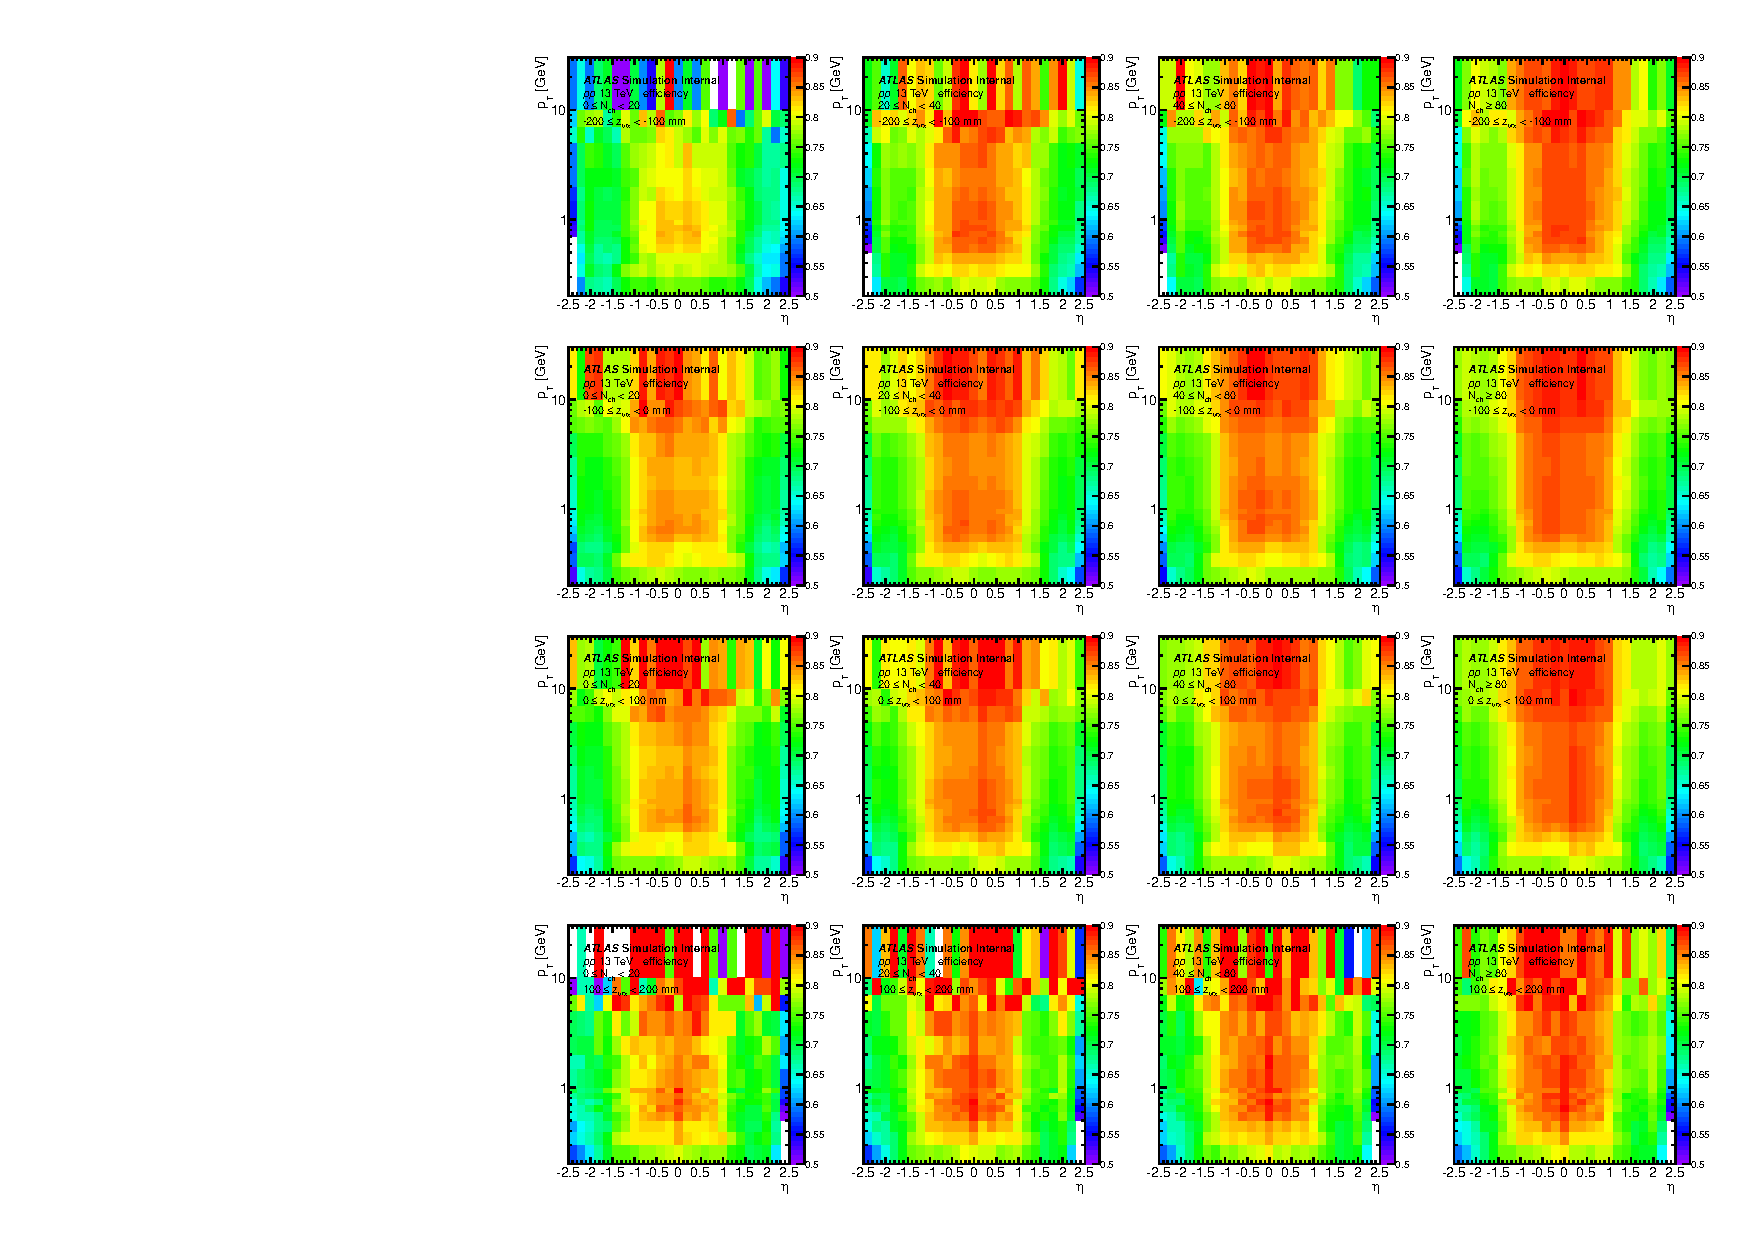
\includegraphics[width=1.\linewidth]{figs/sec_evtSlc/trkEff_pp13_eff_2D_wZvtx.pdf}
\caption{Tracking efficiency $\epsilon(\eta,p_{T})$. Each column is for different $N_{ch}$ ranges, and each row is for different $z_{vtx}$ range.}
\label{fig:trkEff_pp13_eff_2D_wZvtx}
\end{figure}

The efficiency $\epsilon(p_{T},\eta,N_{ch},z_{vtx})$ is summarized in Fig.~\ref{fig:trkEff_pp13_eff_2D_wZvtx}, where different rows represent different $z_{vtx}$ and different columns for different $N_{ch}$ ranges. The efficiency is not uniform in $\eta$: higher in mid$-\eta$ region. It is also not uniform along $p_{T}$: high$-p_{T}$ has higher efficiency. In this analysis, the default $p_{T}$ range is either $0.3<p_{T}<3.0$ GeV or $0.5<p_{T}<5.0$ GeV, and in the plots the $p_{T}$ starts from 0.2 GeV. So the efficiency is in low$-p_{T}$ is still above $60\%$. Moving from low$-N_{ch}$ to high$-N_{ch}$ the efficiency slightly increases: evaluating $\epsilon$ in different $N_{ch}$ is thus required. However, when move from $z_{vtx}~-200$ mm to $z_{vtx}~200$ mm, the efficiency doesn't change much. To gain better statistics, we decide to merge different $z_{vtx}$ ranges when applying efficiency in the data. Besides, since this measurement is not sensitive to rapidity, the minimal changes of the efficiency as a function of $z_{vtx}$ only have negligible impact on the final results.

\begin{figure}[H]
\centering
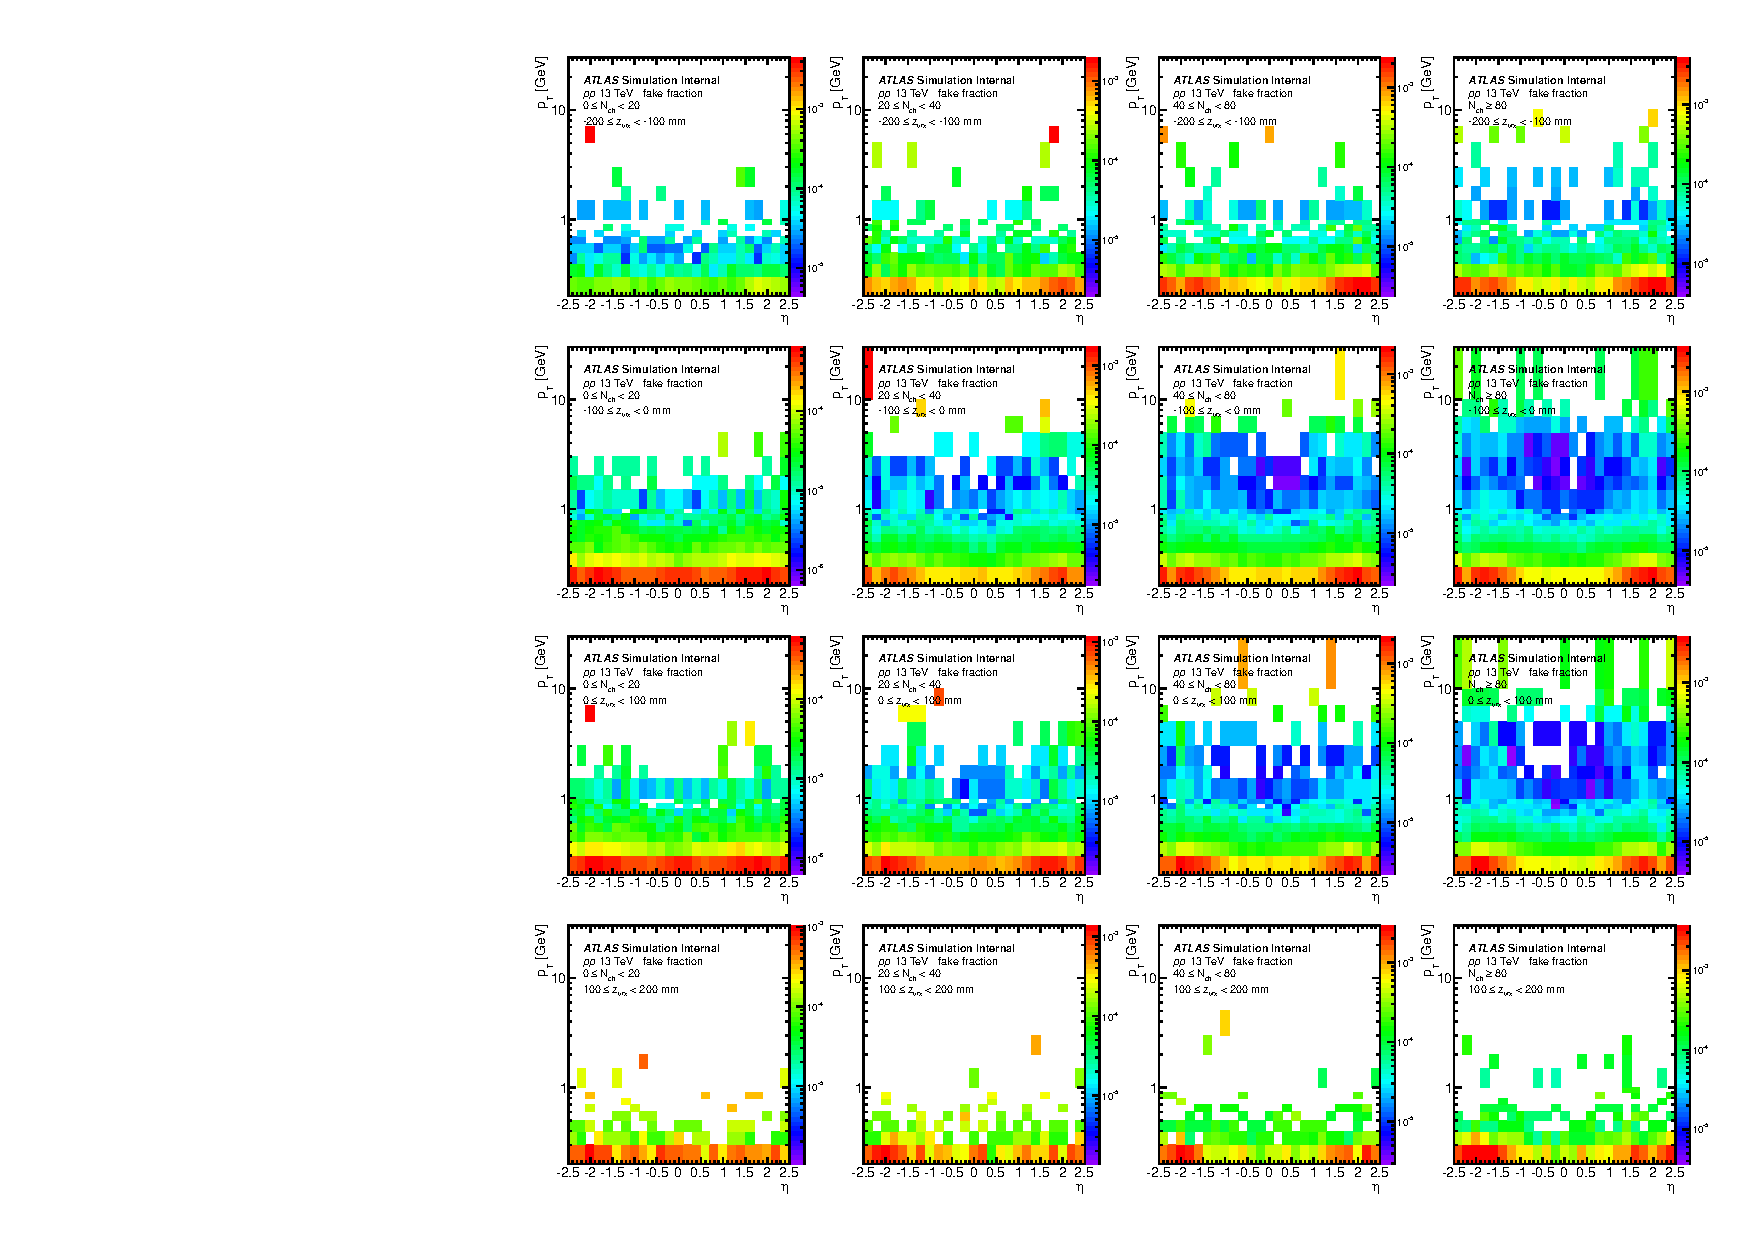
\includegraphics[width=1.\linewidth]{figs/sec_evtSlc/trkEff_pp13_fak_2D_wZvtx.pdf}
\caption{Fake fraction $f(\eta,p_{T})$. Each column is for different $N_{ch}$ ranges, and each row is for different $z_{vtx}$ range.}
\label{fig:trkEff_pp13_fak_2D_wZvtx}
\end{figure}

Fig.~\ref{fig:trkEff_pp13_fak_2D_wZvtx} summaries the fake fraction $f(\eta,p_{T})$ for different $z_{vtx}$ and $N_{ch}$ ranges, where the layouts of the panels are same as previous efficiency plots. The fake fraction is higher in the low$-p_{T}$ region and is consistent with 0 in high$-p_{T}$. The fake fraction is also $\eta$ dependent, but opposite to efficiency: lower in mid-$\eta$. Overall the fake fraction is on the level of below $0.1\%$. Like efficiency, the fake fraction is also dependent of $N_{ch}$, and has very weak dependence of $z_{vtx}$. So we will merge the fake fraction map among different $z_{vtx}$ ranges in the end.

\begin{figure}[H]
\centering
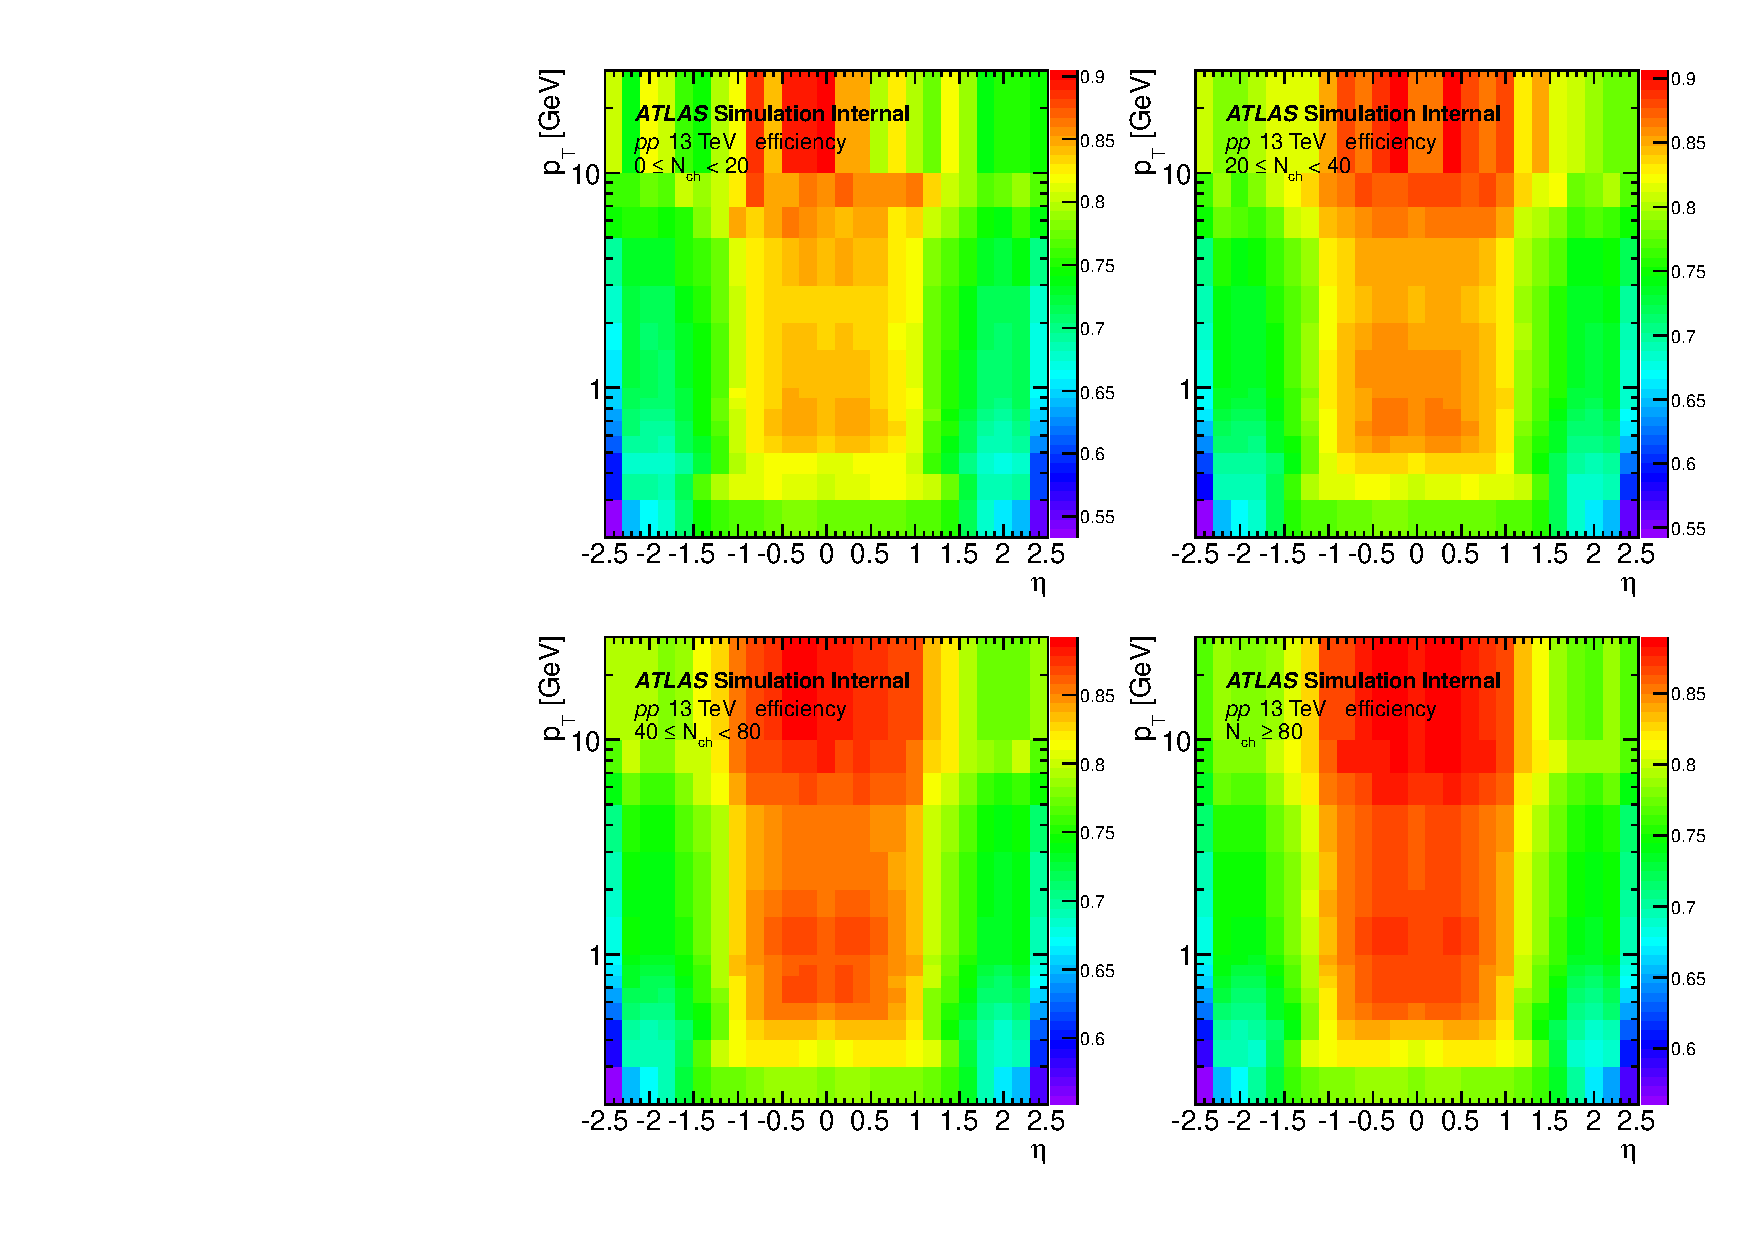
\includegraphics[width=1.\linewidth]{figs/sec_evtSlc/trkEff_pp13_eff_2D.pdf}
\caption{Tracking efficiency $\epsilon(\eta,p_{T})$. Different panels are for different $N_{ch}$ ranges, where different $z_{vtx}$ ranges have been merged.}
\label{fig:trkEff_pp13_eff_2D}
\end{figure}

The merged tracking efficiency is shown in Fig.~\ref{fig:trkEff_pp13_eff_2D}, where four panels are for four different $N_{ch}$ ranges. The boundaries of ranges are chosen to make each range have enough statistics for the efficiency measurement. The efficiency is higher in high multiplicity. These efficiency maps are applied in this analysis, where linear interpolation is used to obtain the more precise efficiency when $p_{\text{T}}$ or $\eta$ are not in the bin center. The $c_{2}{4}$ are compared with using tracking efficiency from previous cumulant measurement and the results are consistent.

\begin{figure}[H]
\centering
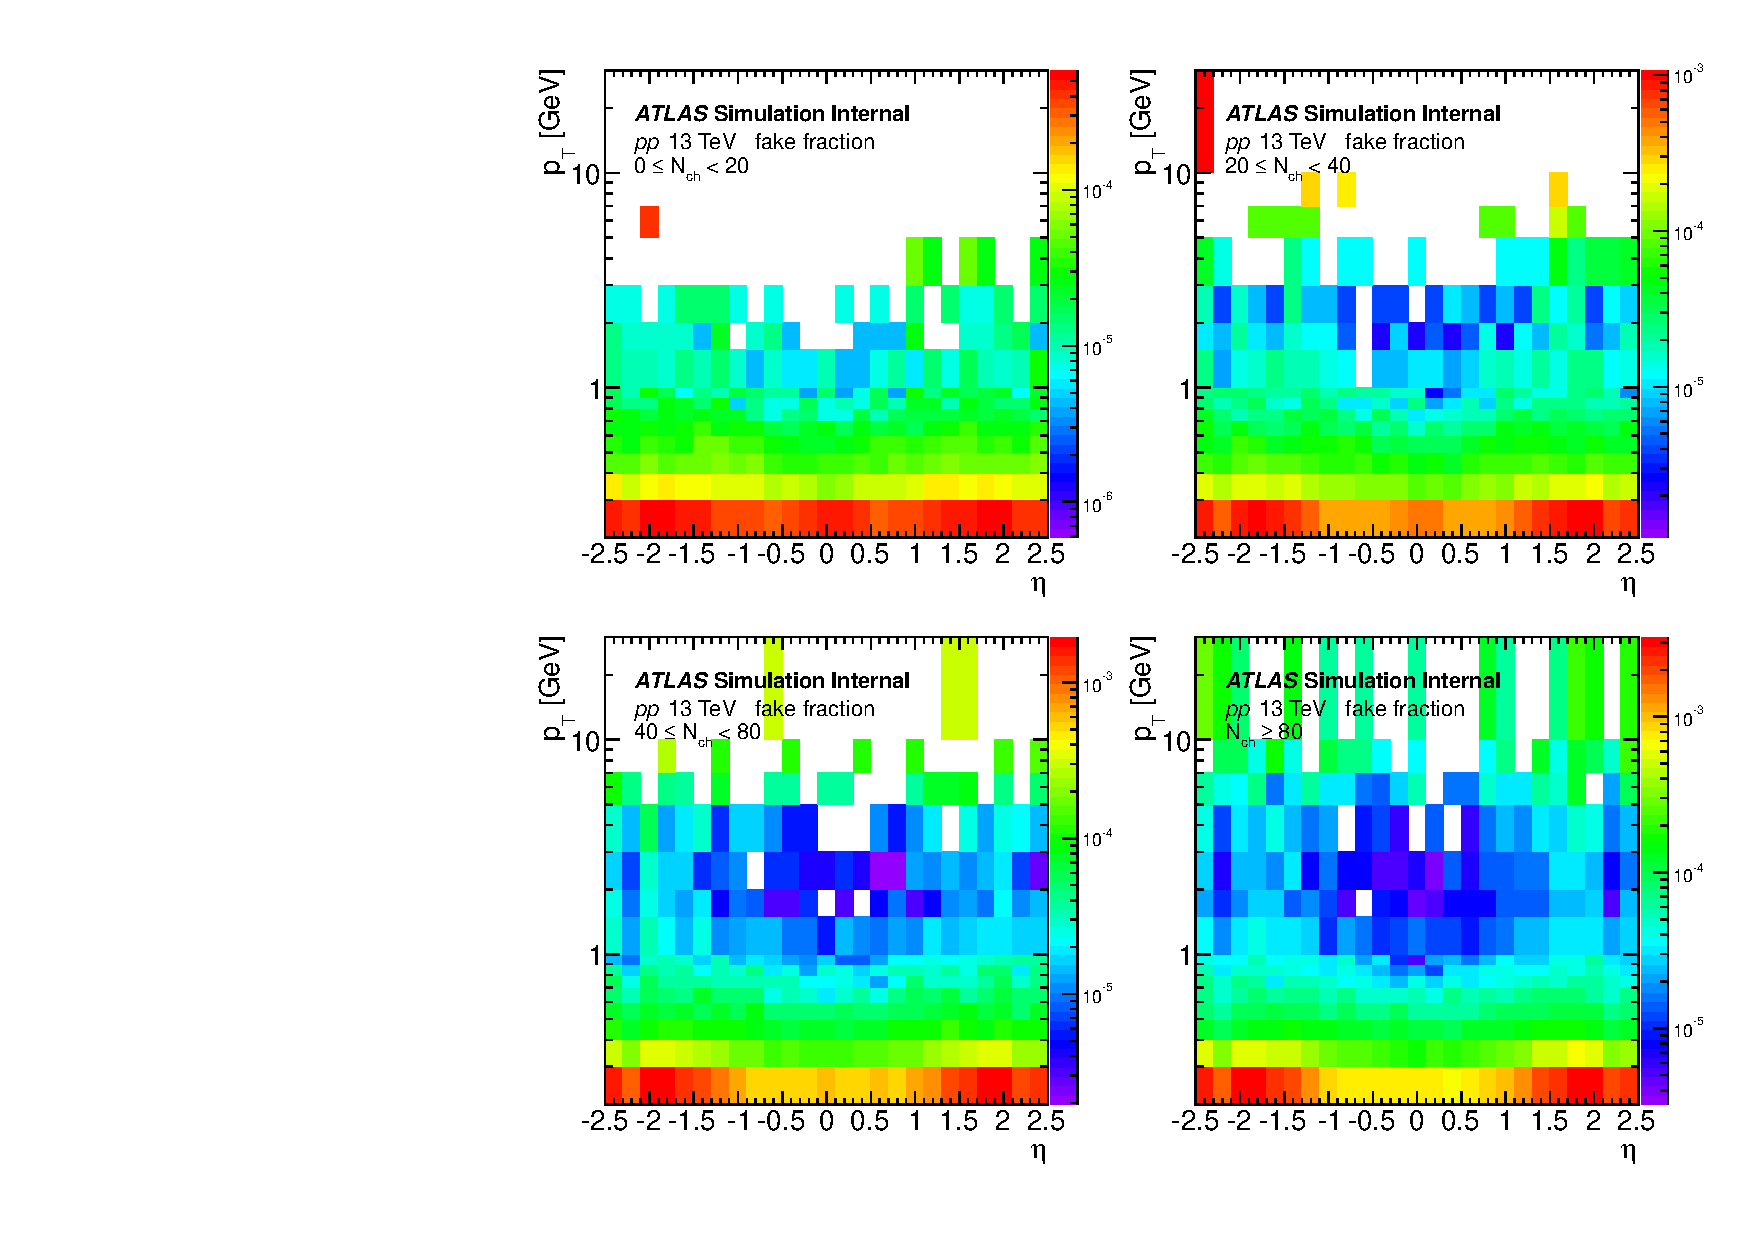
\includegraphics[width=1.\linewidth]{figs/sec_evtSlc/trkEff_pp13_fak_2D.pdf}
\caption{Fake fraction $f(\eta,p_{T})$. Different panels are for different $N_{ch}$ ranges, where different $z_{vtx}$ ranges have been merged.}
\label{fig:trkEff_pp13_fak_2D}
\end{figure}

The merged fake fraction is shown in Fig.~\ref{fig:trkEff_pp13_fak_2D}, where four panels are for four different $N_{ch}$ ranges. Since the maximum fake fraction is smaller than the level of $0.1\%$, even for the lowest $p_{T}$, we will not apply this additional correction in the data analysis.

In the systematics section we will test the stability of the results by varying the tracking efficiency.

Appendix~\ref{sec:appdx} summarizes many detailed monitoring plots for this PYTHIA sample.



\subsubsection{Tracking validation for run 305359, 309314 and 309346}
When producing the GRL for the low-$\mu$ $pp$ runs in 2016, three runs are tagged with following issues:
\begin{itemize}
\item Run 305359: \verb|BTAG_BLAYER_SERIOUS_PROBLEM|
\item Run 309314: \verb|ID_BS_RUNAVERAGE|
\item Run 309346: \verb|ID_BS_RUNAVERAGE|
\end{itemize}
where in run 305359, the IBL detector is absent while in the other two runs, there is no constrain on the beam spot position at the trigger level. (The offline reconstruction DOES impose the beam spot constraint in all runs.) When beam spot is constraint, fluctuation of rate of HMT triggers has been observed, due to online reconstruction issues.

The purpose of this section is to validate the basic tracking quantities in these three runs, to check whether IBL and beam spot can have an impact on the results. Run 310216 is used as a reference for comparison. All the events are required to pass the MB trigger \verb|HLT_mb_sptrk| and the track selection is identical to the $pp$ analysis.

\begin{figure}[H]
\centering
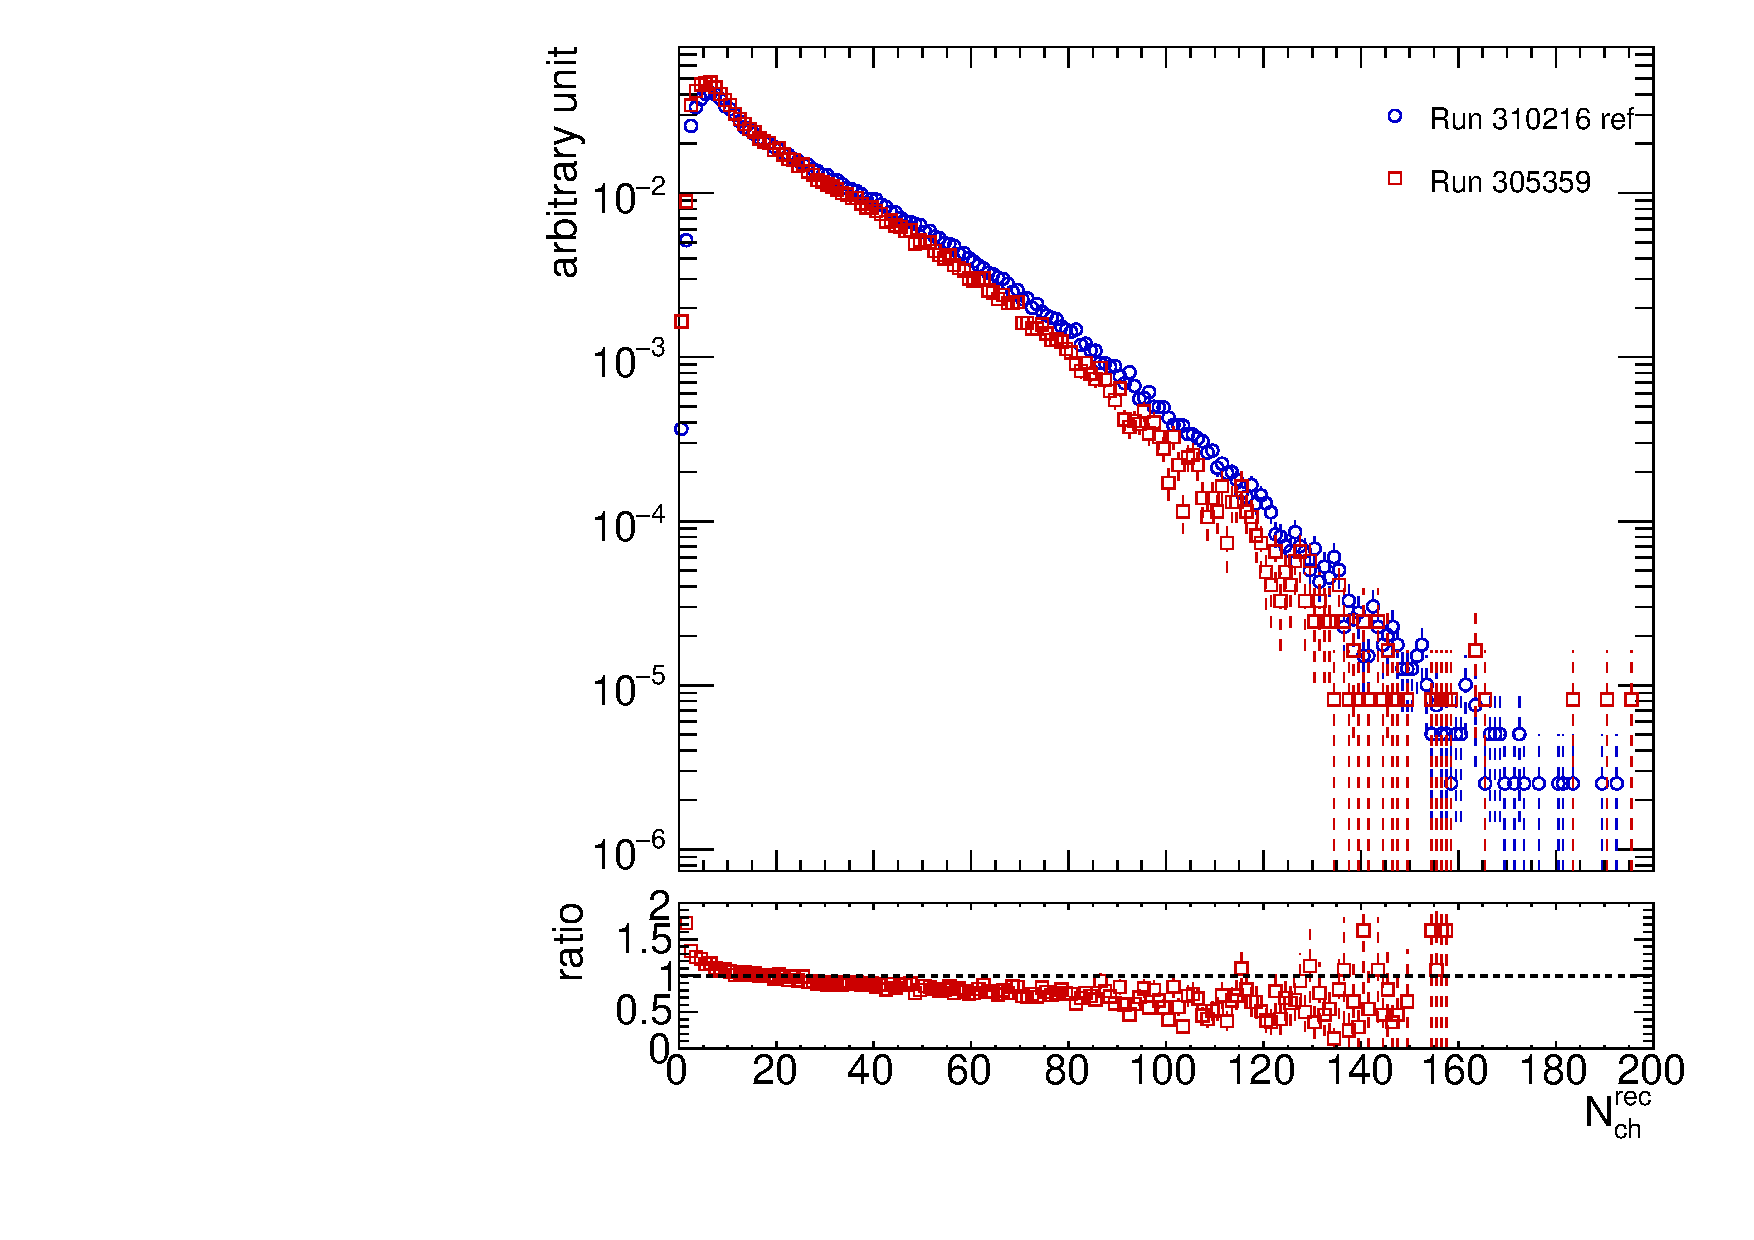
\includegraphics[width=0.45\linewidth]{figs/sec_evtSlc/GRLpp2016/305359_dis_nTrk.pdf}
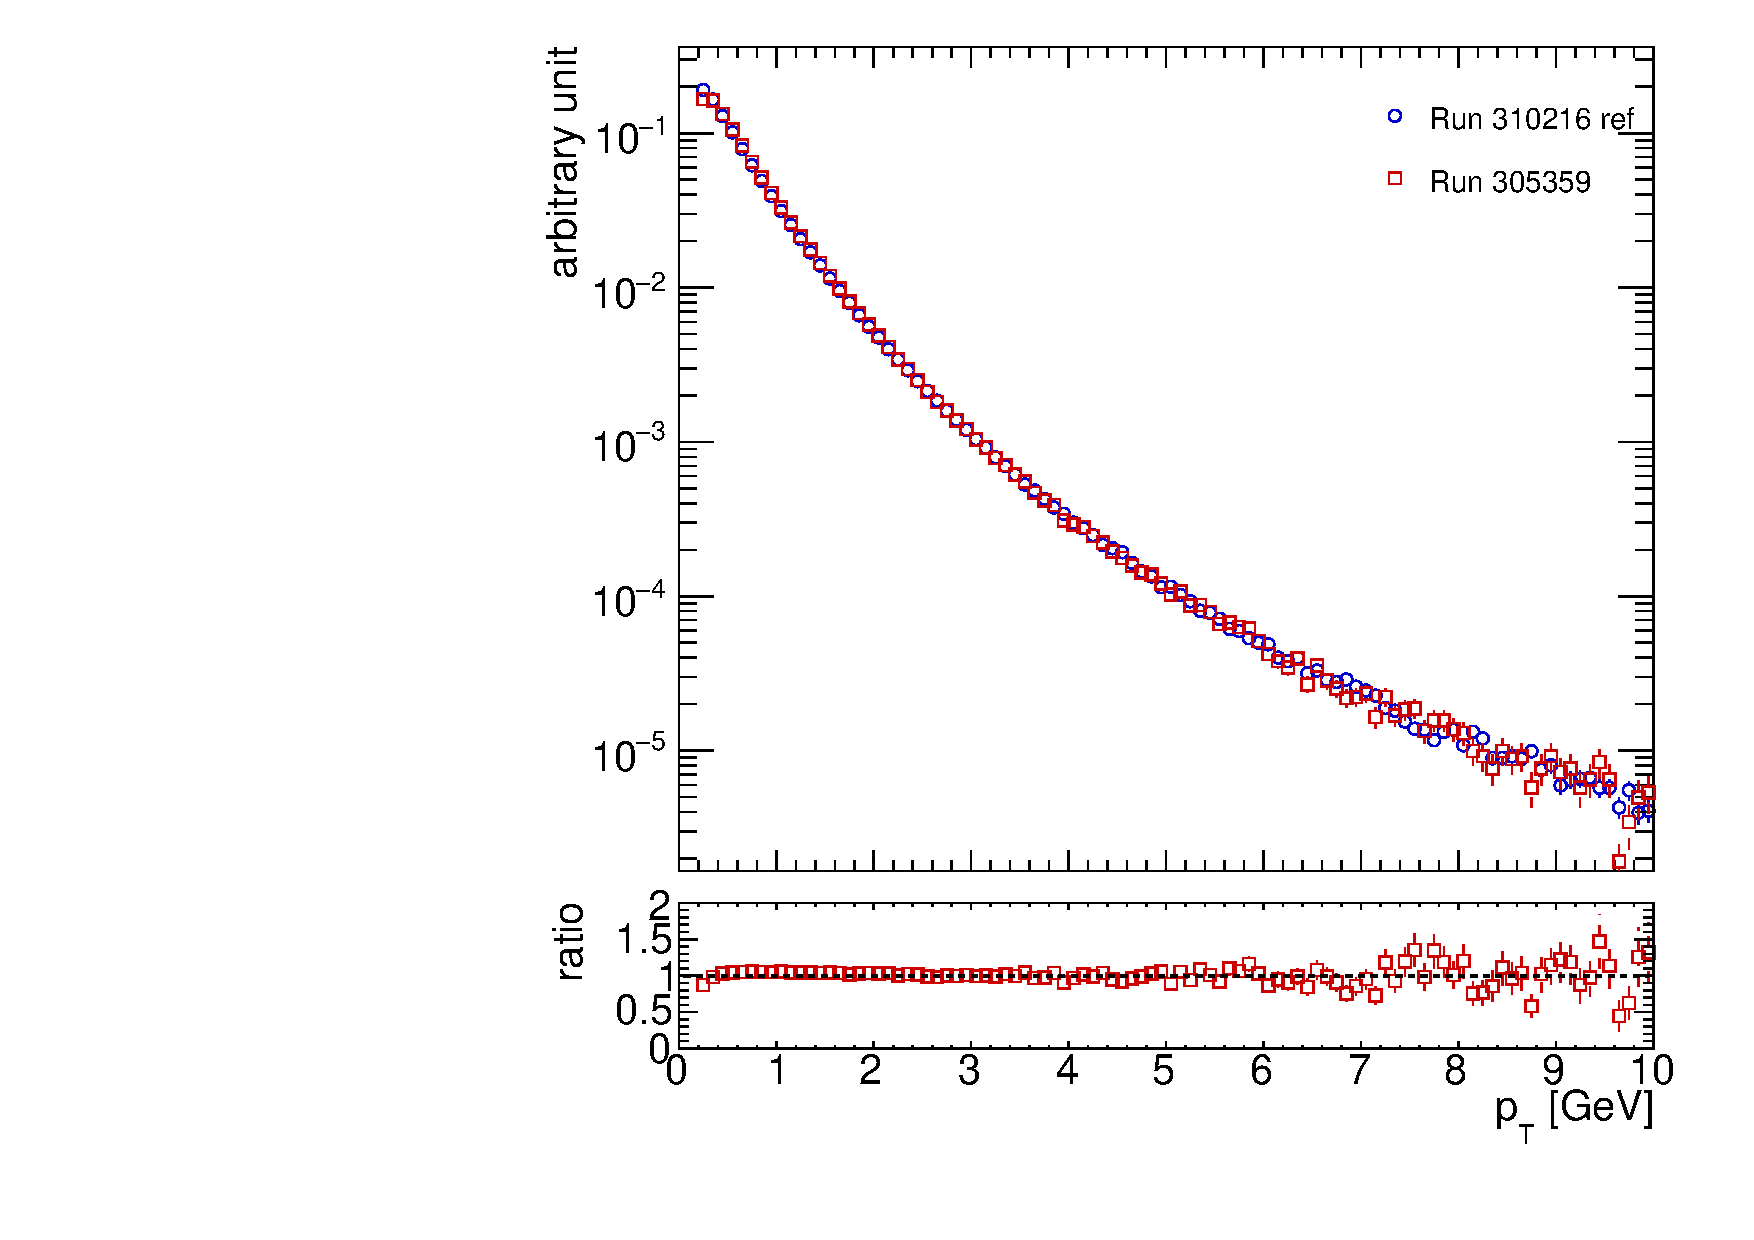
\includegraphics[width=0.45\linewidth]{figs/sec_evtSlc/GRLpp2016/305359_dis_pt.pdf}
\caption{Distribution of number of offline reconstructed tracks and $p_{\text{T}}$ spectrum: a comparison between run 305359 and run 310216.}
\label{fig:GRLpp2016_305359_nTrk_pt}
\end{figure}
Fig.~\ref{fig:GRLpp2016_305359_nTrk_pt} shows the comparison of number of reconstructed tracks distribution and $p_{\text{T}}$ spectrum, between run 305359 and 310216. The mean value of number of tracks is slightly smaller in 305359 than 310216. This is probably due to that the IBL is absent in 305359, and same cut on number of Pixel hits will reject slightly more events in this run. Meanwhile, the $p_{\text{T}}$ spectrums are consistent between the two runs, except for the lowest $p_{\text{T}}$ region, where again it is due to the absence of IBL detector, thus the tracking reconstruction has a poorer efficiency in the lowest $p_{\text{T}}$ region. We will come back to this behavior again once we show the comparison of Run 1 and Run 2 $p$+Pb tracking efficiency.

\begin{figure}[H]
\centering
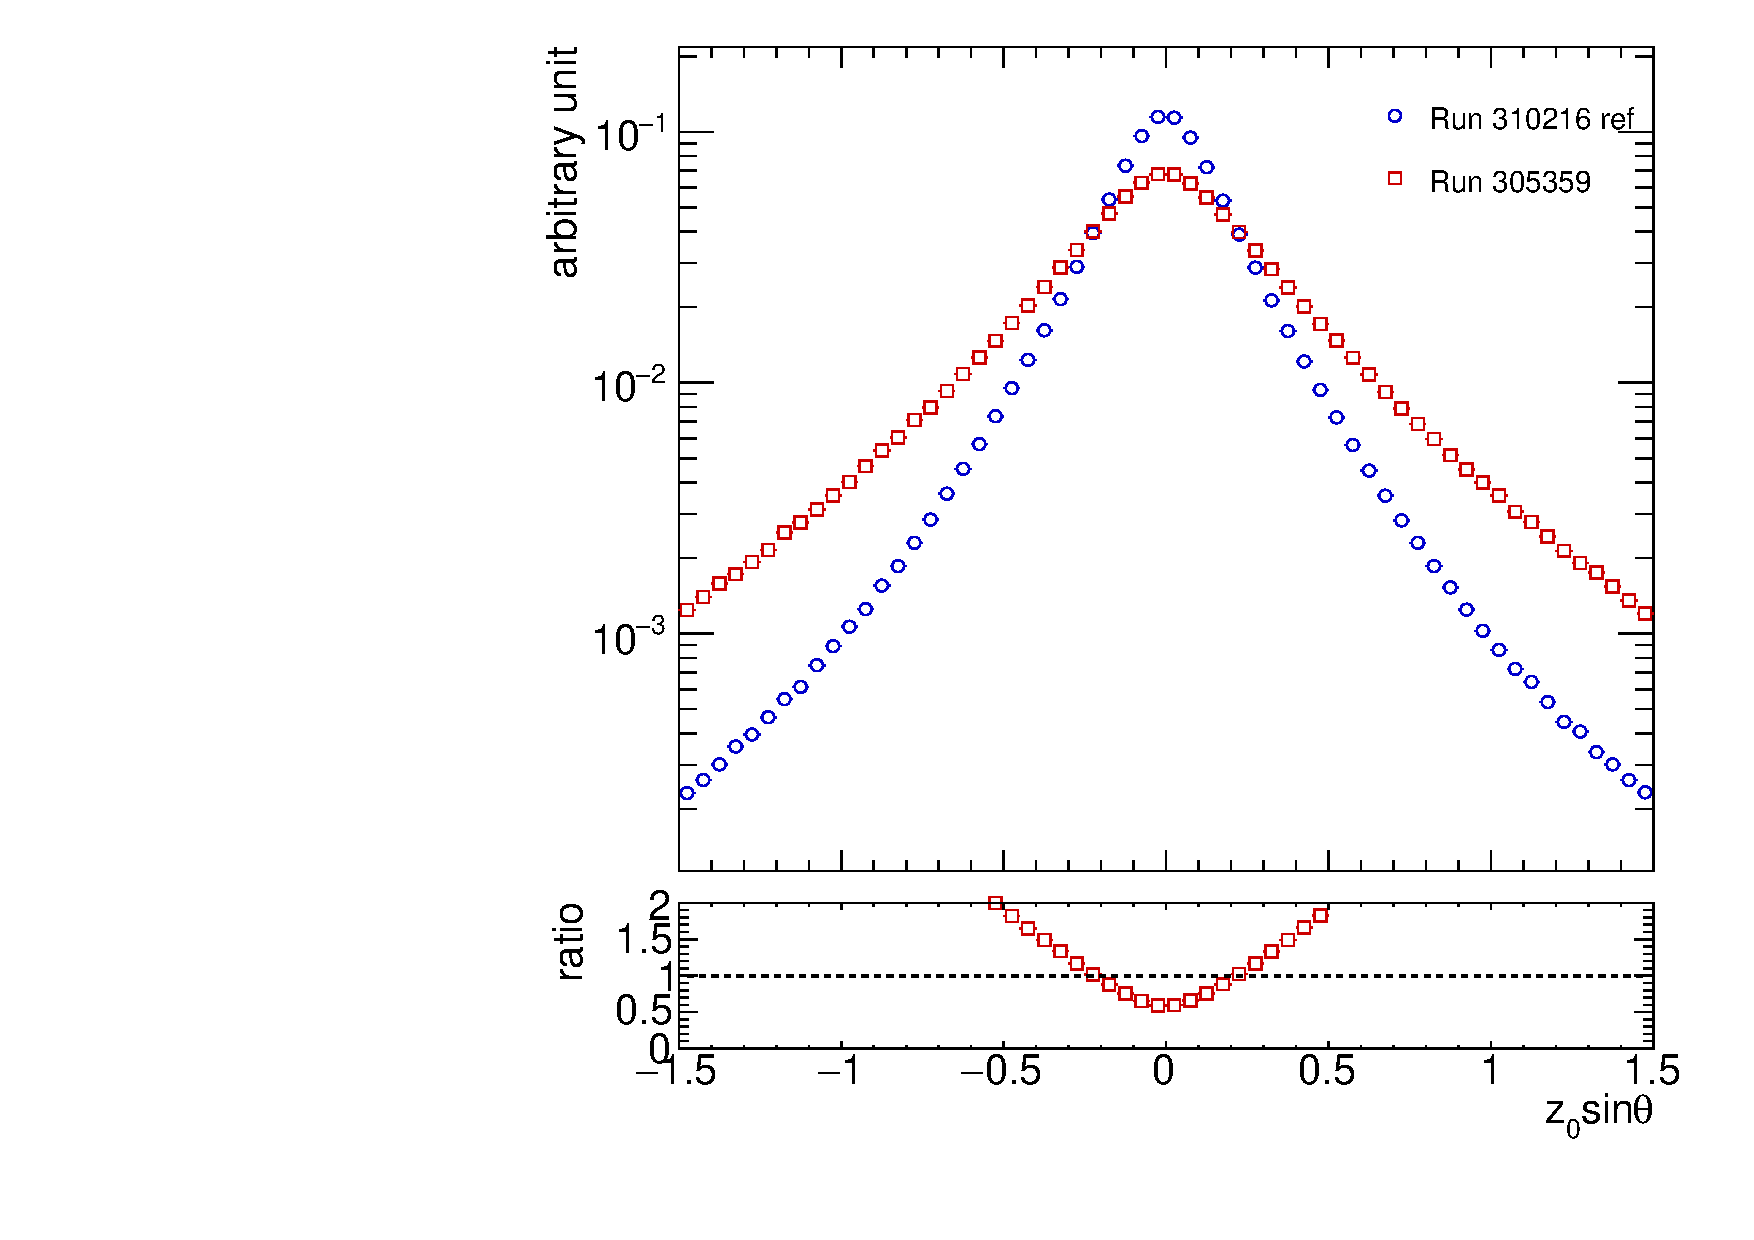
\includegraphics[width=0.45\linewidth]{figs/sec_evtSlc/GRLpp2016/305359_dis_z0.pdf}
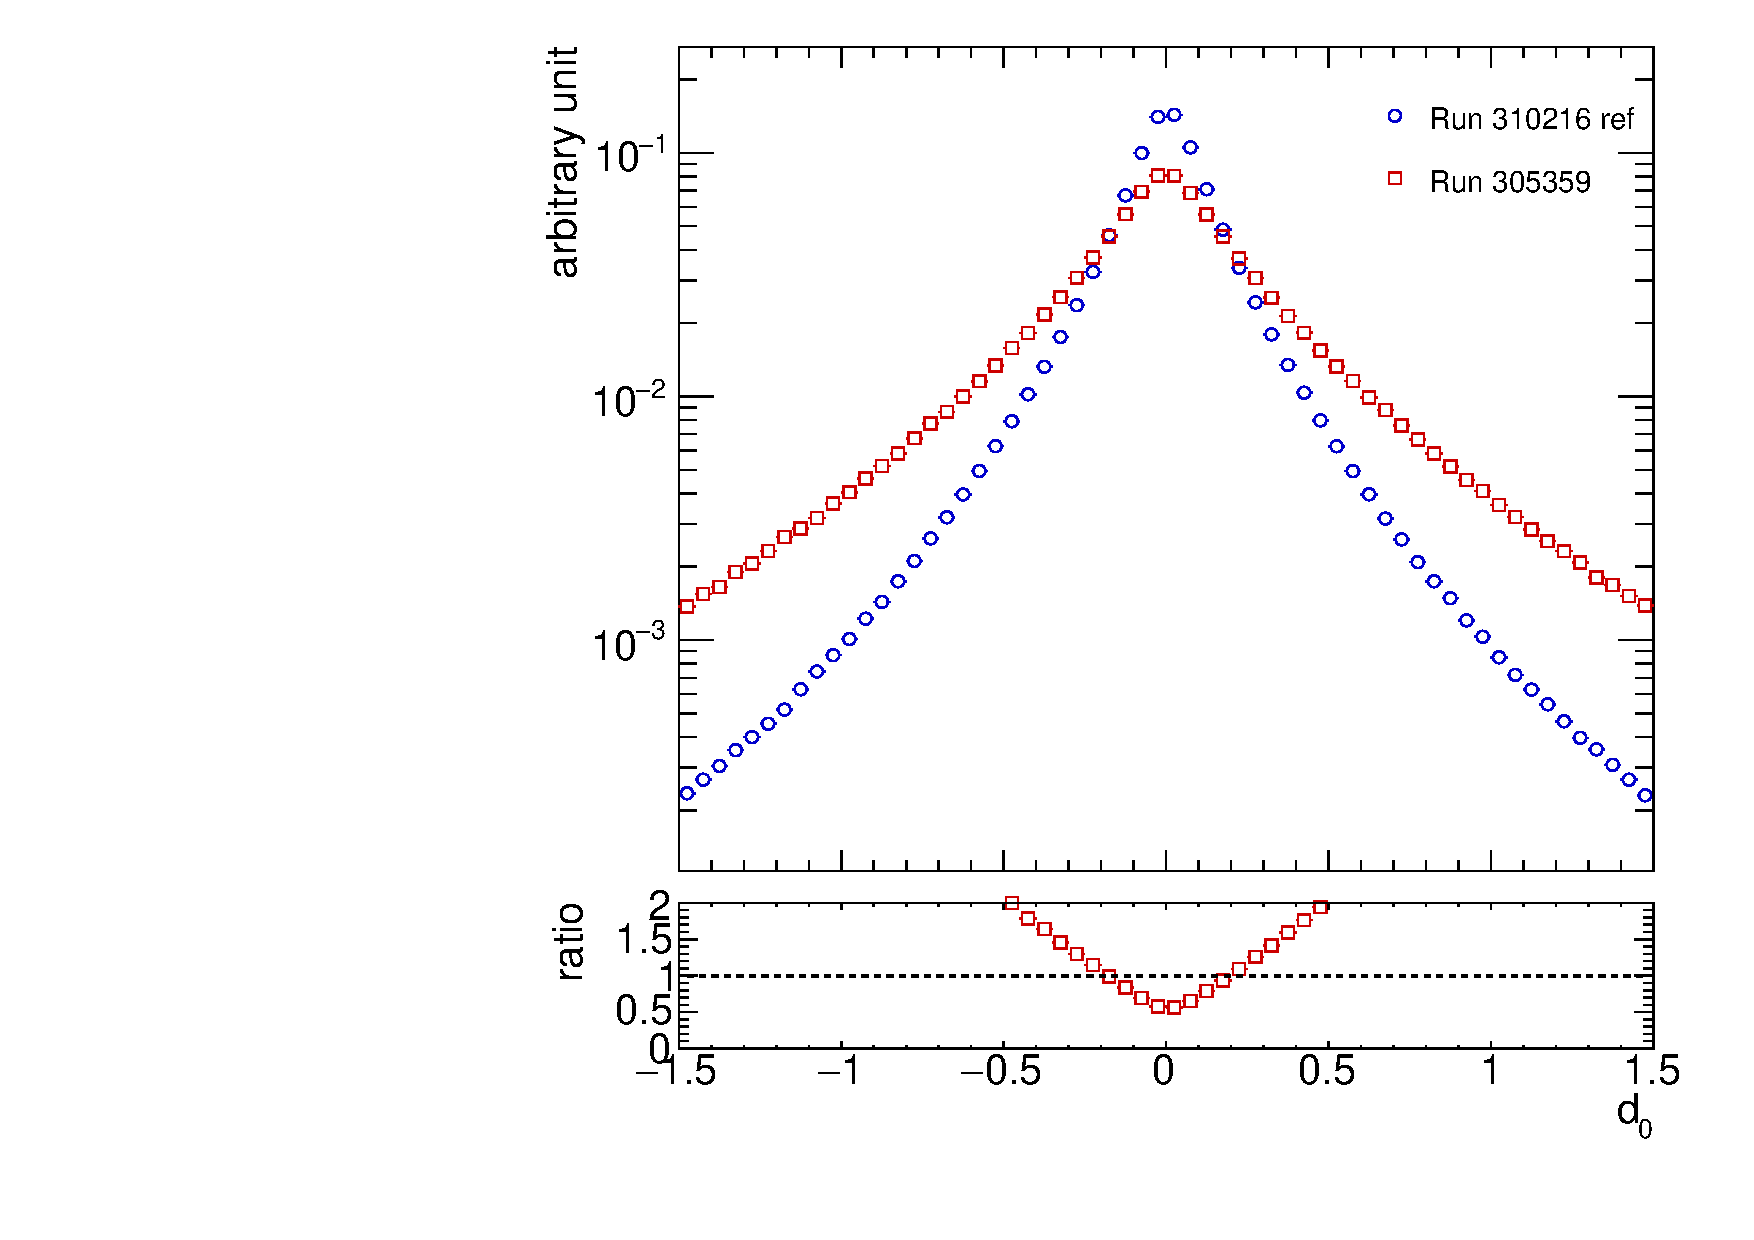
\includegraphics[width=0.45\linewidth]{figs/sec_evtSlc/GRLpp2016/305359_dis_d0.pdf}
\caption{Distribution of $z_{0}\text{sin}\theta$ and $d_{0}$ of reconstructed tracks: a comparison between run 305359 and run 310216.}
\label{fig:GRLpp2016_305359_z0_d0}
\end{figure}
Fig.~\ref{fig:GRLpp2016_305359_z0_d0} shows the comparison of $z_{0}\text{sin}\theta$ and $d_{0}$ distribution of reconstructed tracks, between run 305359 and 310216. Both $z_{0}$ and $d_{0}$ distributions are much wider when IBL is absent. The default tracking pointing cut is at 1.5 mm, which will result in different tracks because of the different $z_{0}$ and $d_{0}$ distribution.

\begin{figure}[H]
\centering
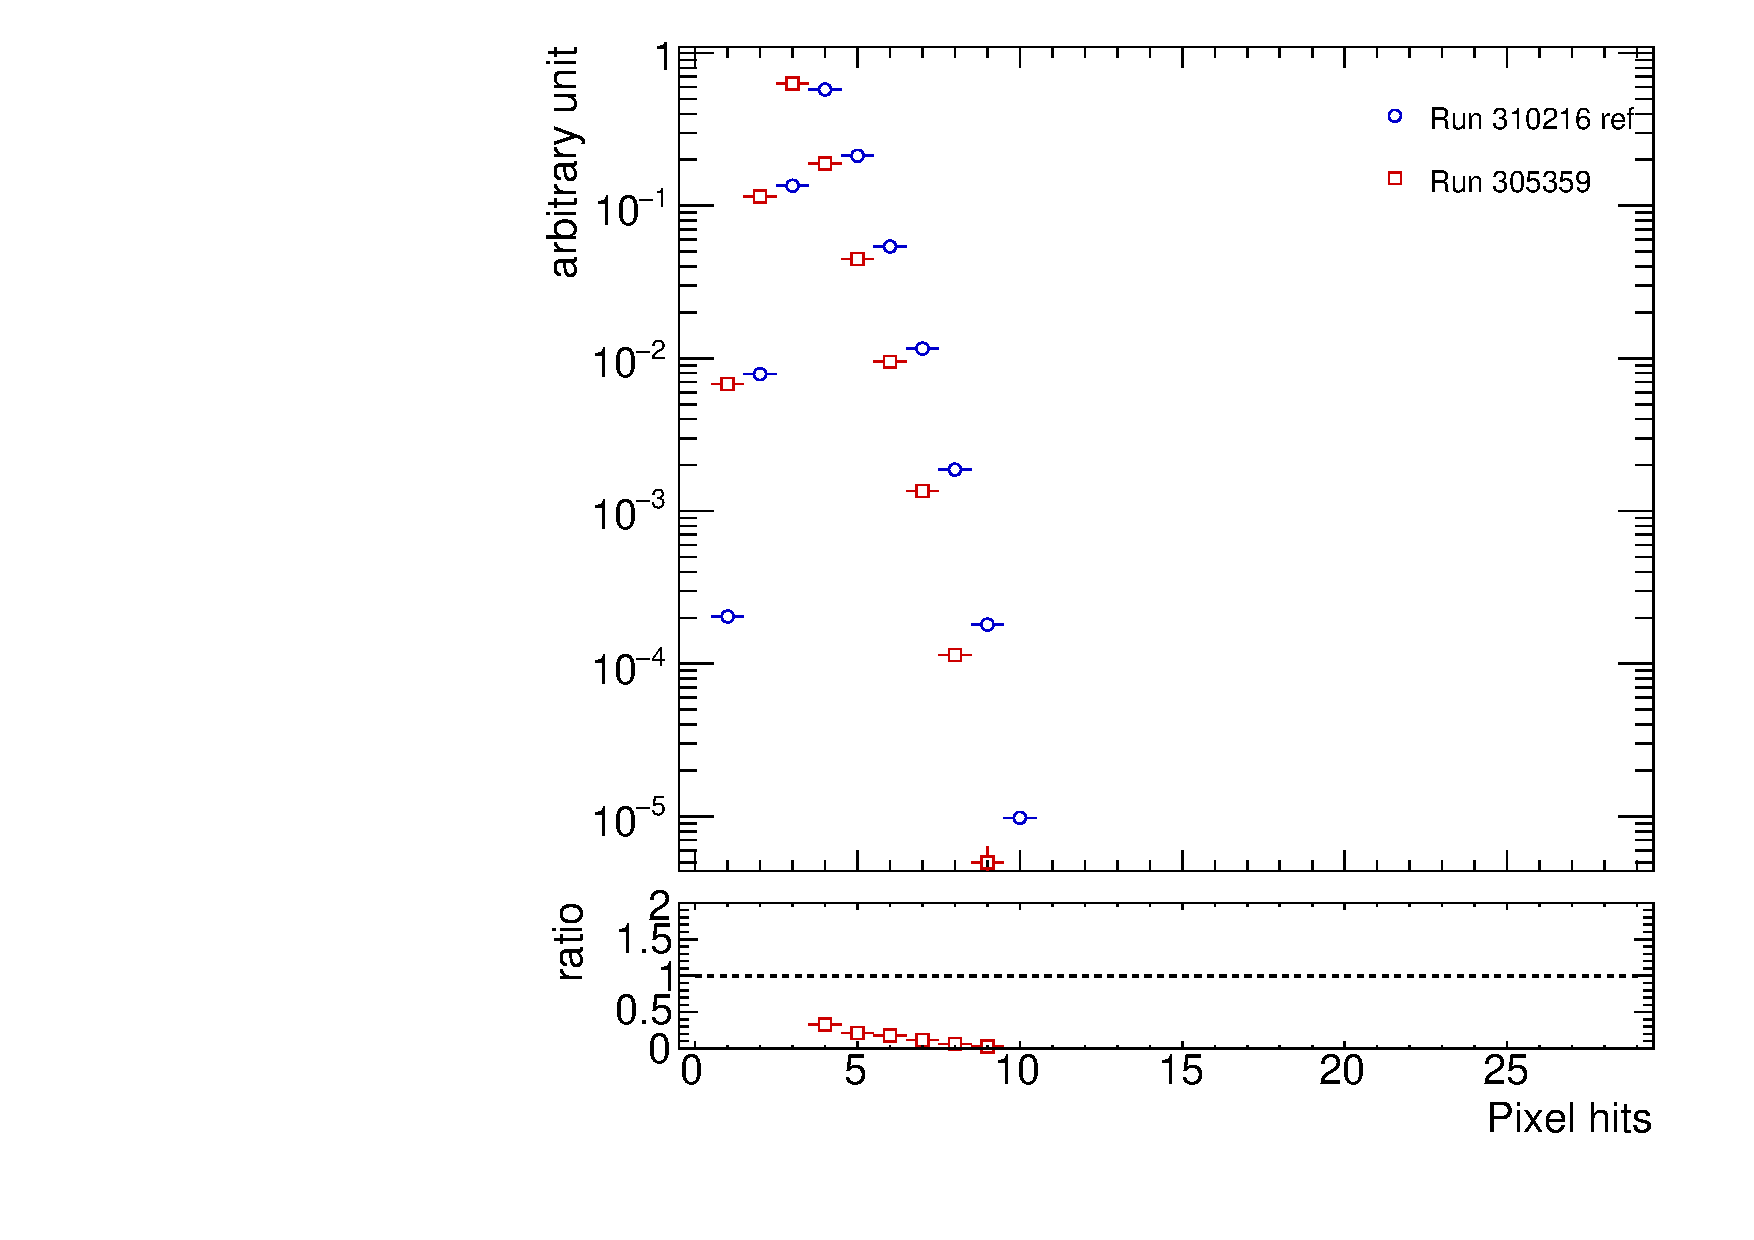
\includegraphics[width=0.45\linewidth]{figs/sec_evtSlc/GRLpp2016/305359_dis_pixHit.pdf}
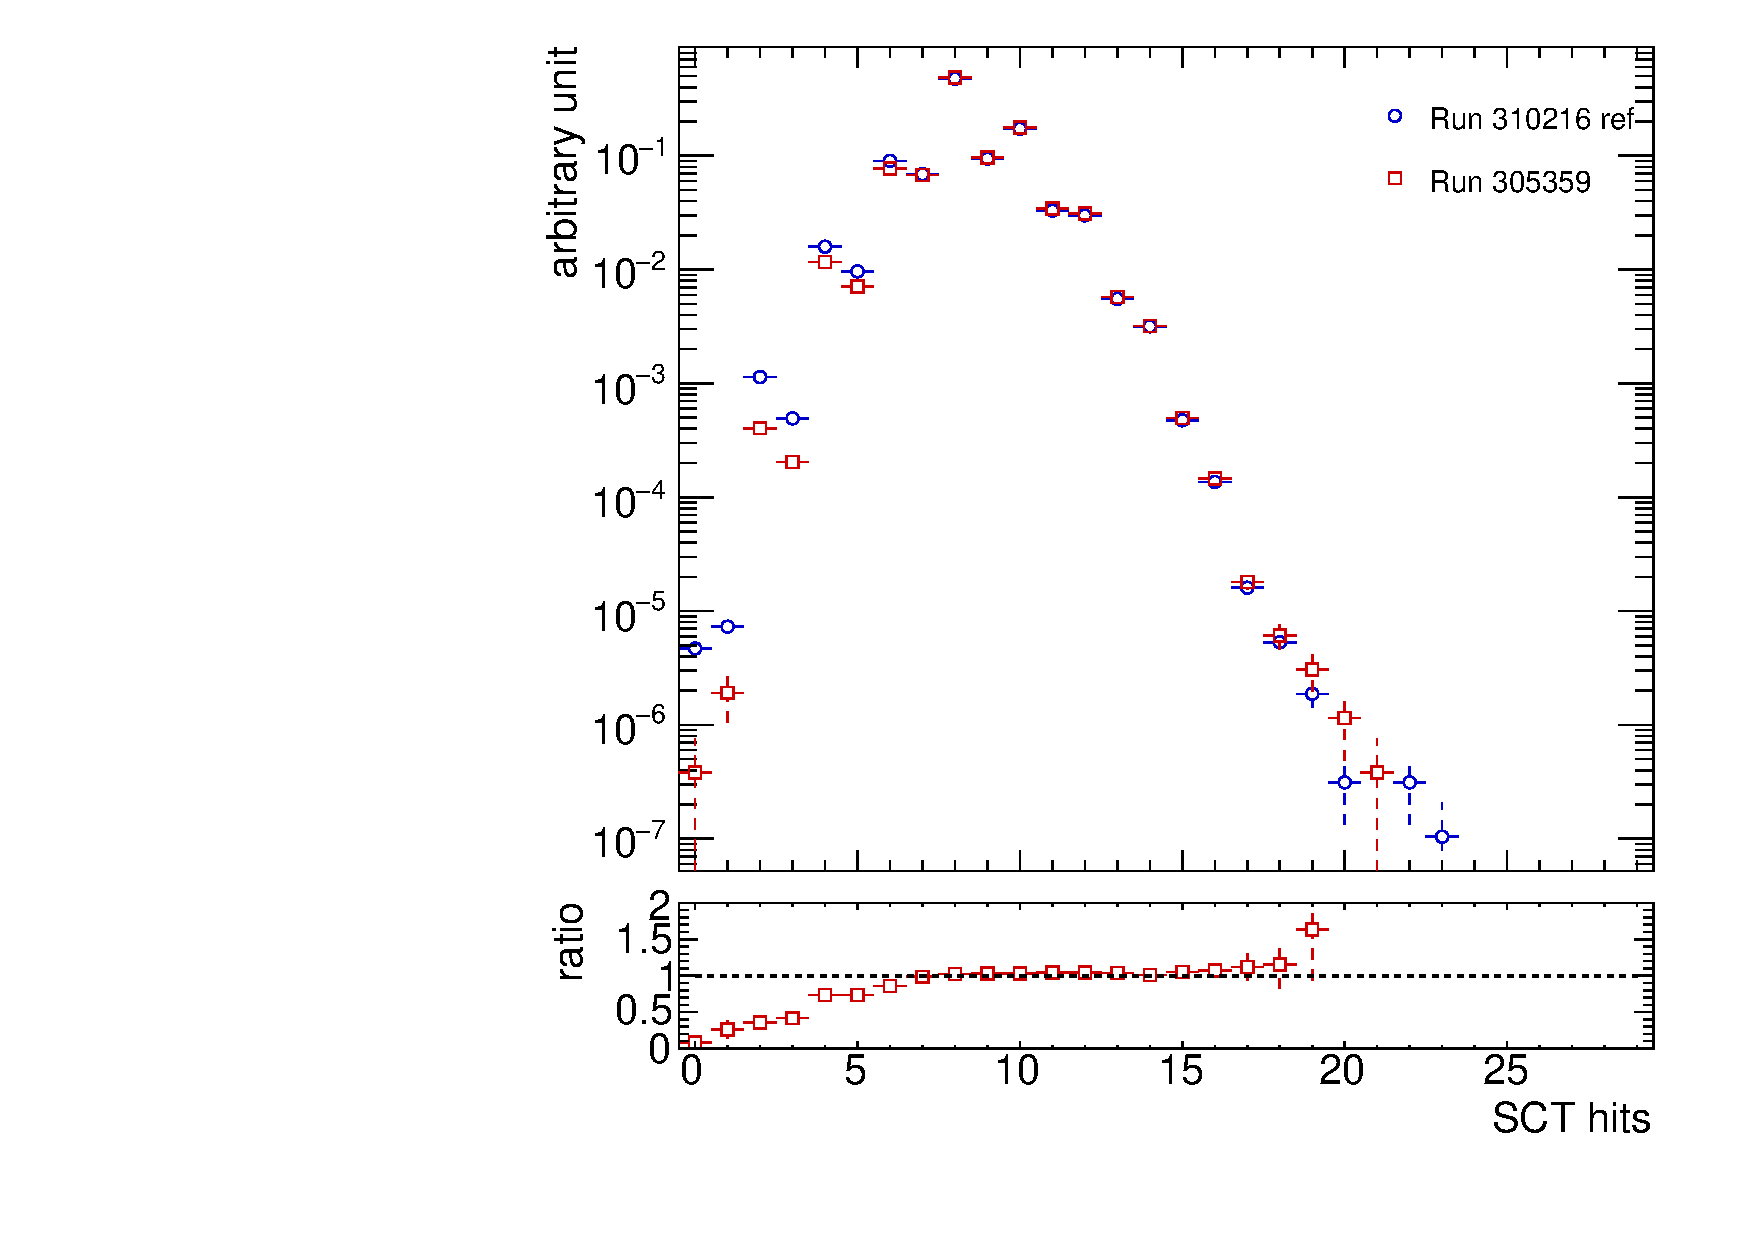
\includegraphics[width=0.45\linewidth]{figs/sec_evtSlc/GRLpp2016/305359_dis_sctHit.pdf}
\caption{Distribution of number of Pixel and SCT hits of reconstructed tracks: a comparison between run 305359 and run 310216.}
\label{fig:GRLpp2016_305359_pixHit_sctHit}
\end{figure}
Fig.~\ref{fig:GRLpp2016_305359_pixHit_sctHit} shows the comparison of number of Pixel and SCT hits, between run 305359 and 310216. Due to absence of IBL, the number of Pixel hits in run 305359 is shifted by 1 compared with 310216. The number of SCT hits are consistent between the two runs, above the default track selection cut.

\begin{figure}[H]
\centering
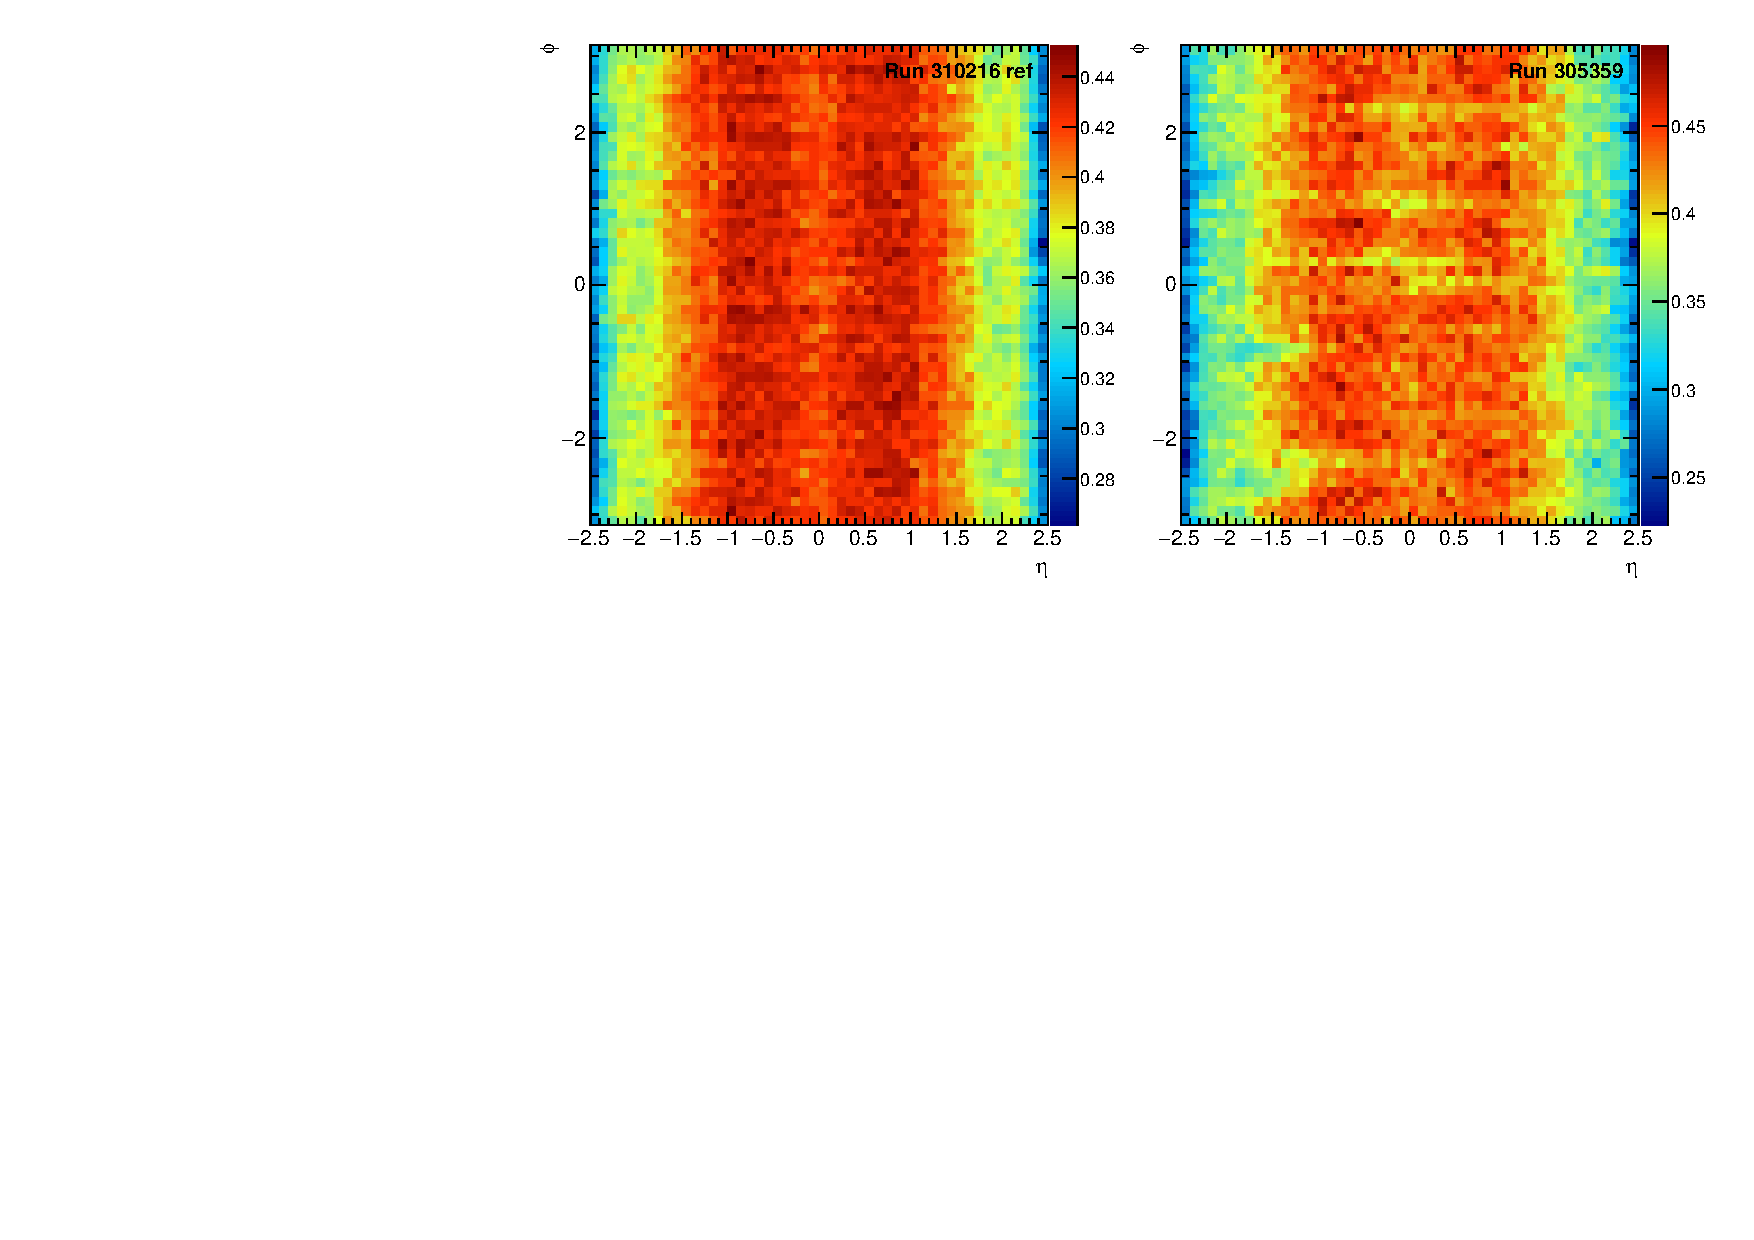
\includegraphics[width=0.9\linewidth]{figs/sec_evtSlc/GRLpp2016/305359_crr_eta_phi.pdf}
\caption{2D map of raw $\eta$-$\phi$ distribution: a comparison between run 305359 and run 310216.}
\label{fig:GRLpp2016_305359_eta_phi}
\end{figure}
Finally, fig.~\ref{fig:GRLpp2016_305359_eta_phi} shows the 2D map of raw $\eta$-$\phi$ distribution. "raw" means the tracks are not weighted by tracking efficiency. The distribution is much more uniform in run 310216 than 305359.

As a conclusion, because of the absence of IBL, $z_{0}$, $d_{0}$ and $\eta$-$\phi$ distributions are quite different between run 310216 and 305359. In principle, most of the differences can be covered by a dedicated Monte-Carlo sample with special detector setup for the run 305359. However, after discussion with the experts who prepared the GRL, we decide not to include run 305359, which only contributes to less than 10$\%$ of the total statistics.

\begin{figure}[H]
\centering
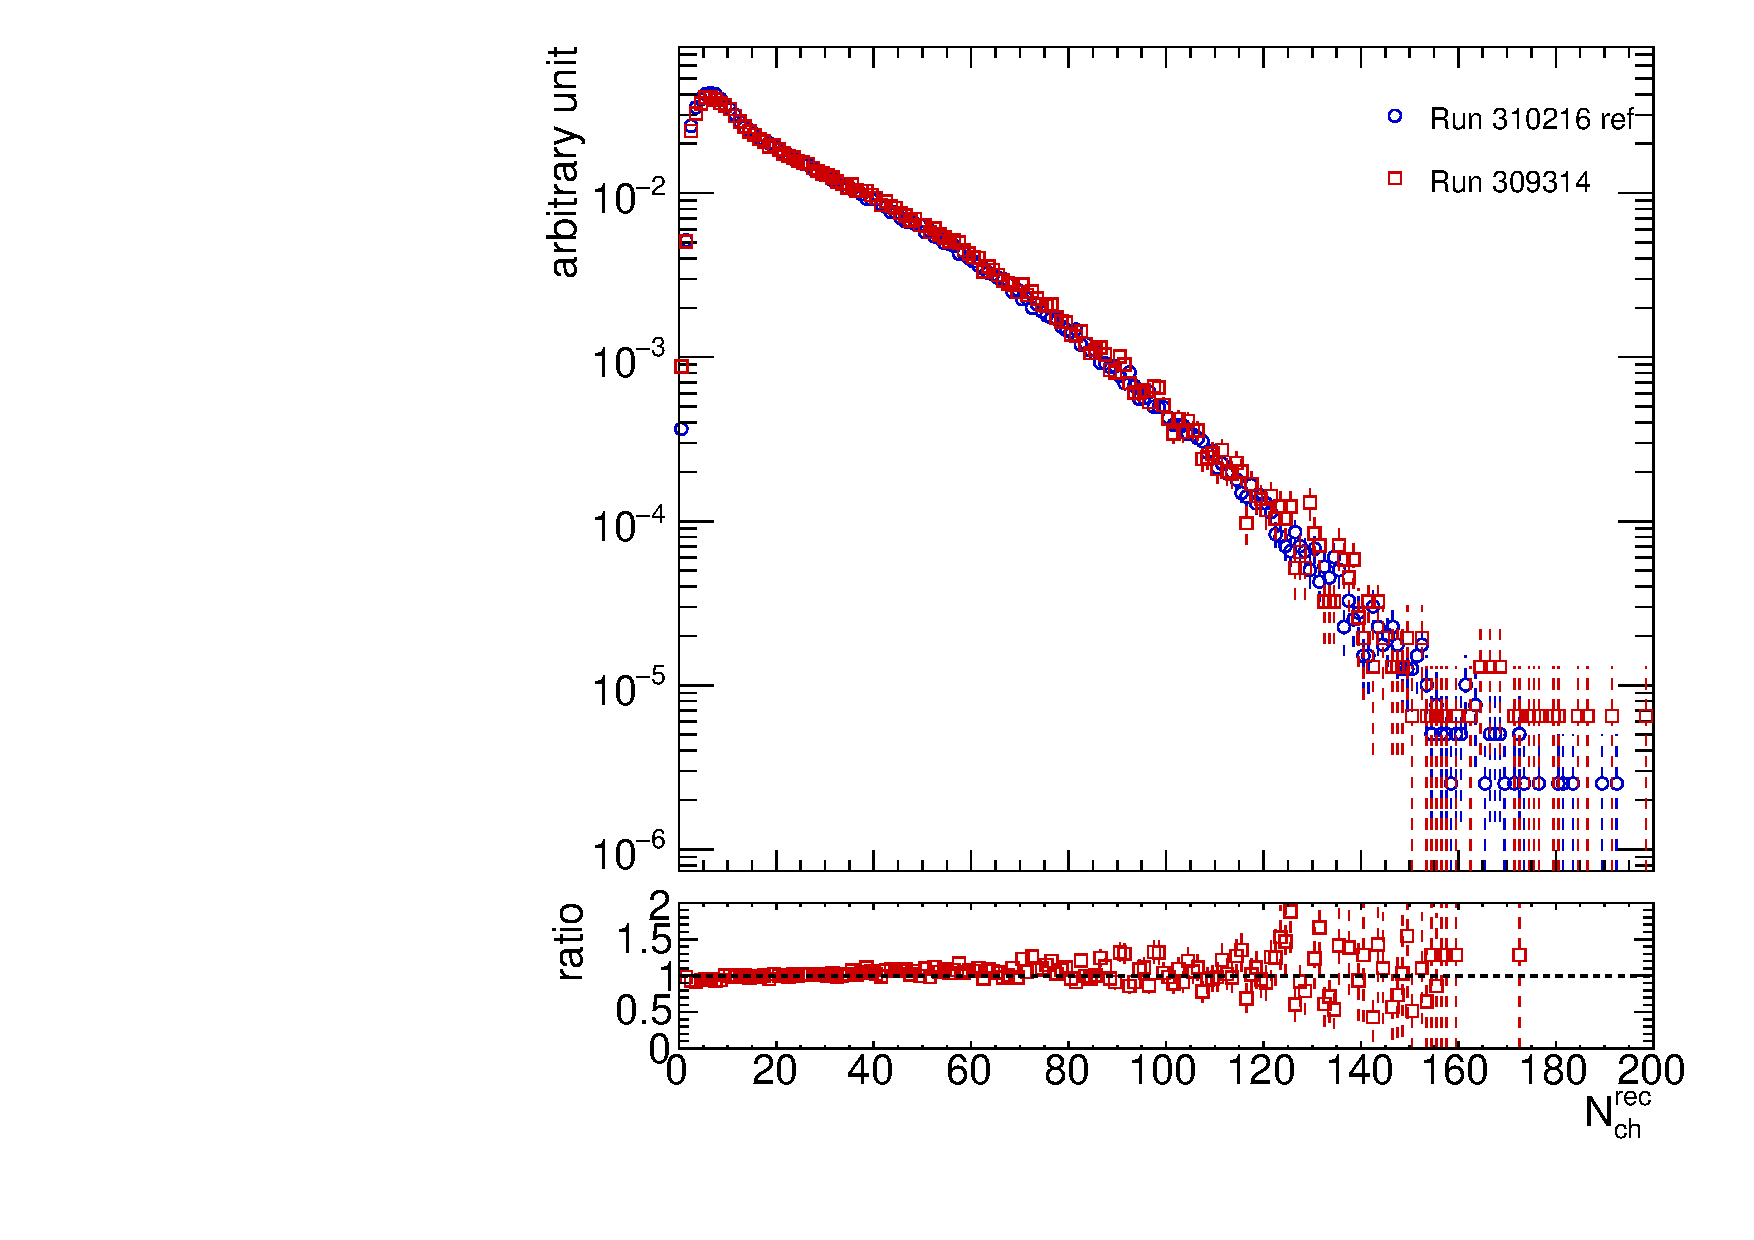
\includegraphics[width=0.45\linewidth]{figs/sec_evtSlc/GRLpp2016/309314_dis_nTrk.pdf}
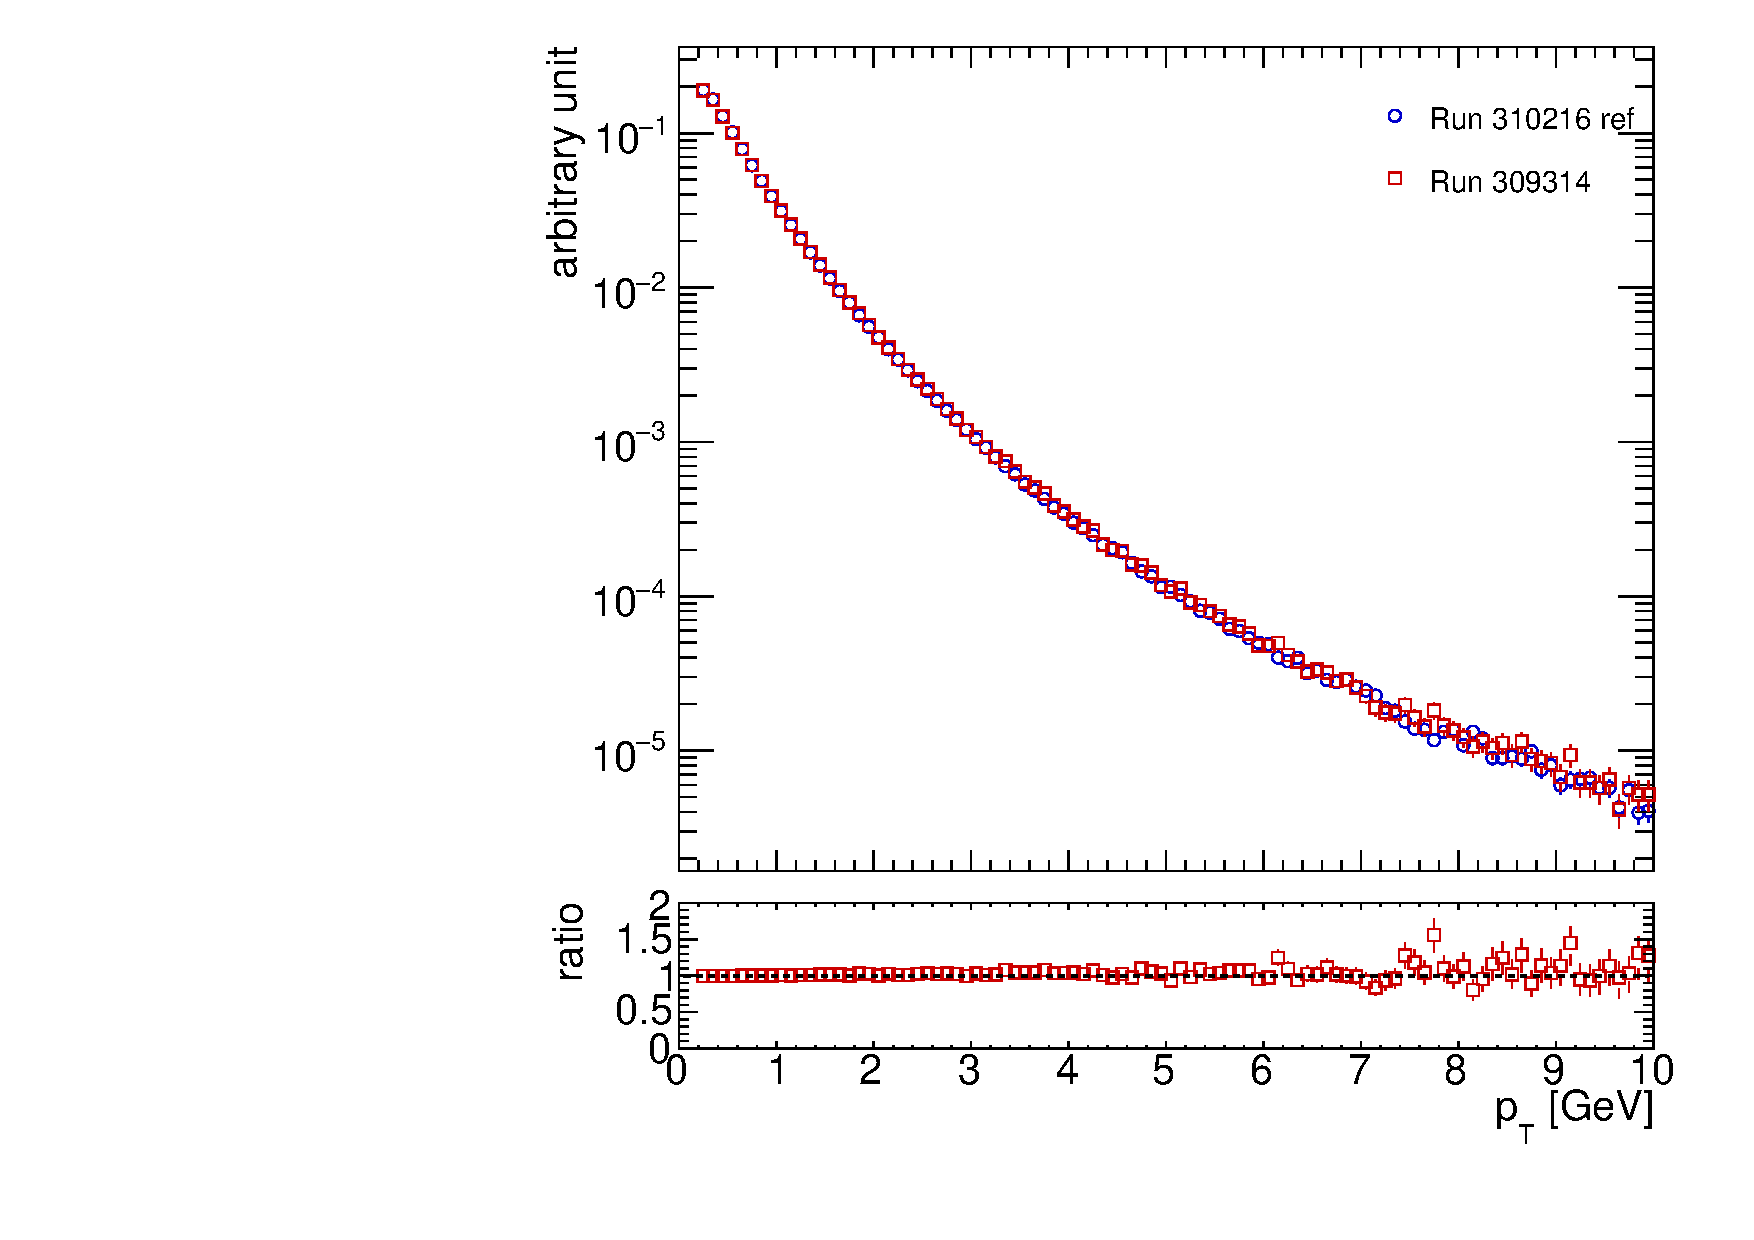
\includegraphics[width=0.45\linewidth]{figs/sec_evtSlc/GRLpp2016/309314_dis_pt.pdf}
\caption{Distribution of number of offline reconstructed tracks and $p_{\text{T}}$ spectrum: a comparison between run 309314 and run 310216.}
\label{fig:GRLpp2016_309314_nTrk_pt}
\end{figure}
The rest two runs are tagged with the error \verb|ID_BS_RUNAVERAGE|, since the beam spot position is not constraint. In the following we will demonstrate that tracking quantities will be consistent without beam spot constraint. Fig.~\ref{fig:GRLpp2016_309314_nTrk_pt} shows the comparison of number of reconstructed tracks distribution and $p_{\text{T}}$ spectrum, between run 309314 and 310216. The ratios show that they are very consistent.

\begin{figure}[H]
\centering
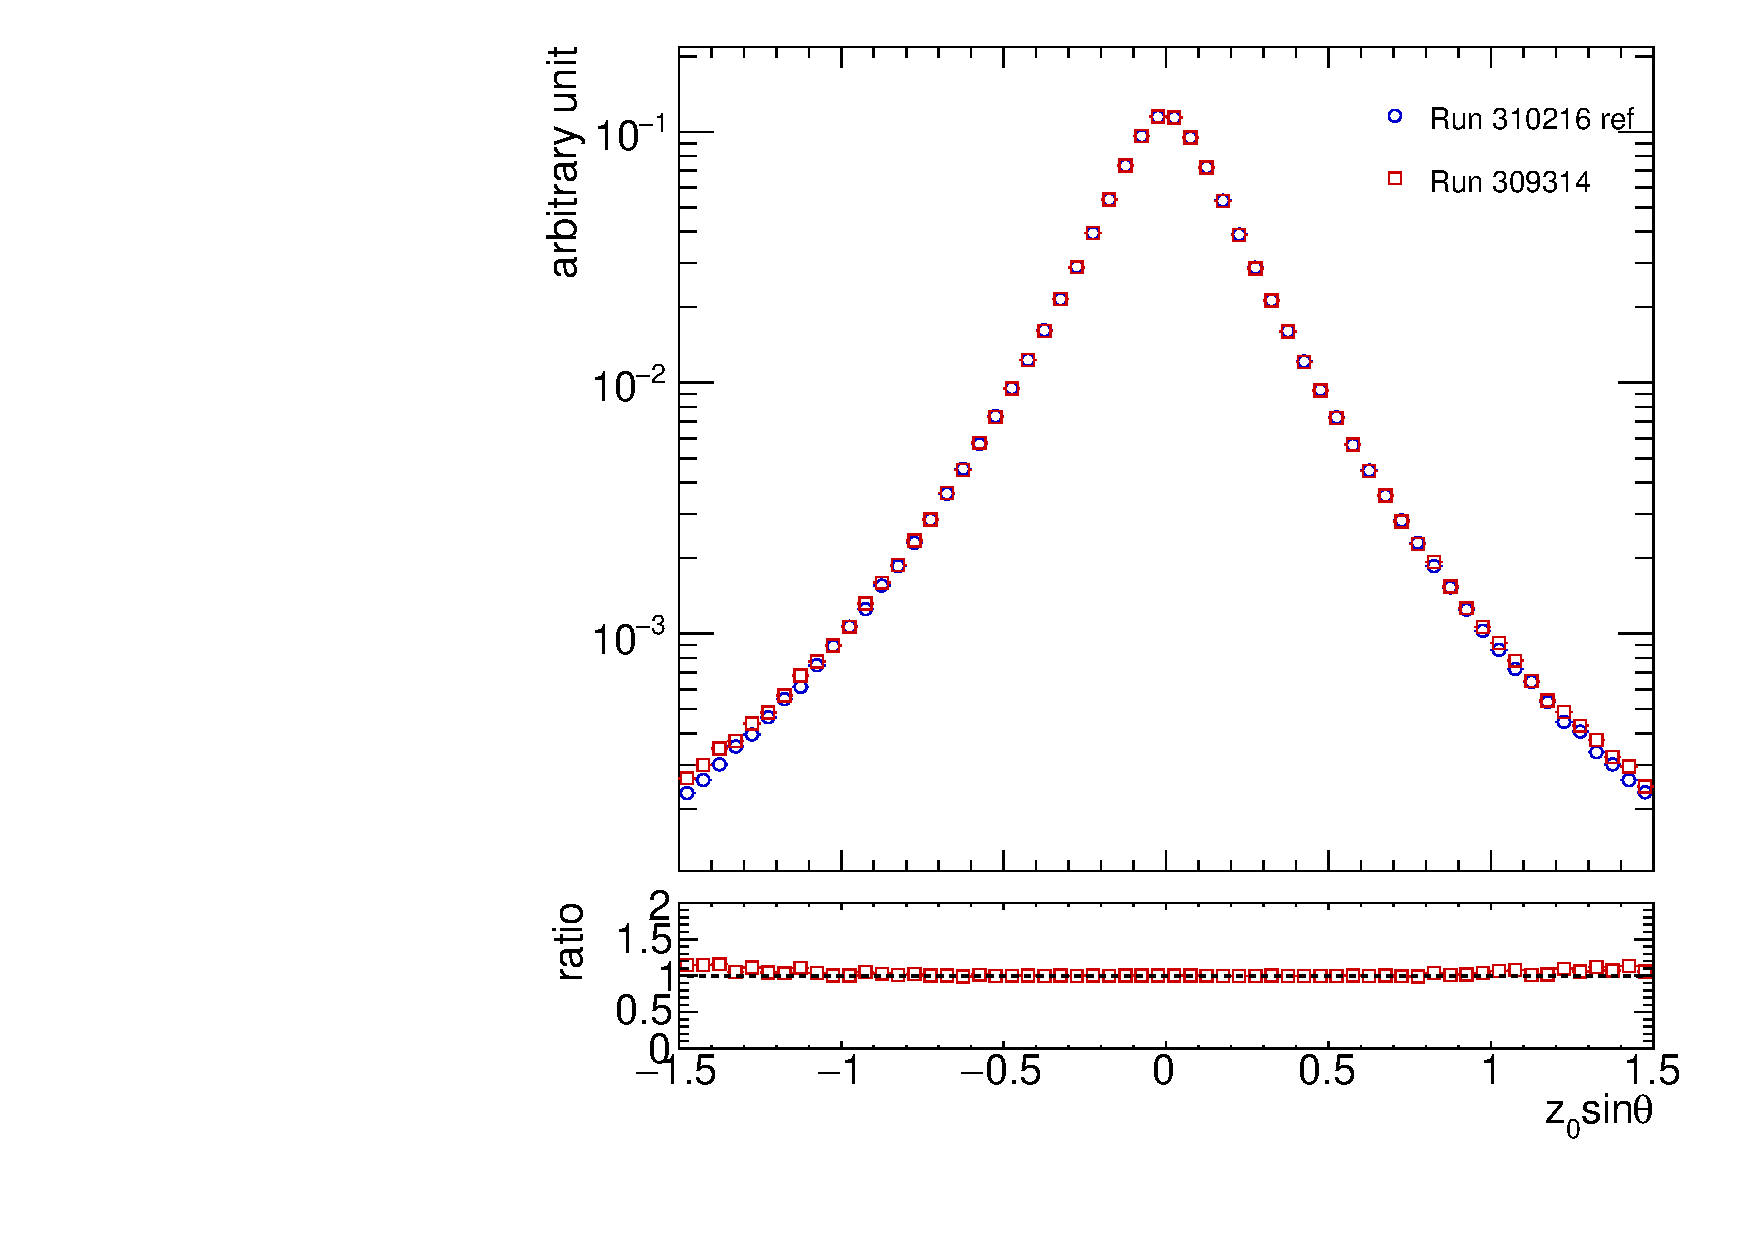
\includegraphics[width=0.45\linewidth]{figs/sec_evtSlc/GRLpp2016/309314_dis_z0.pdf}
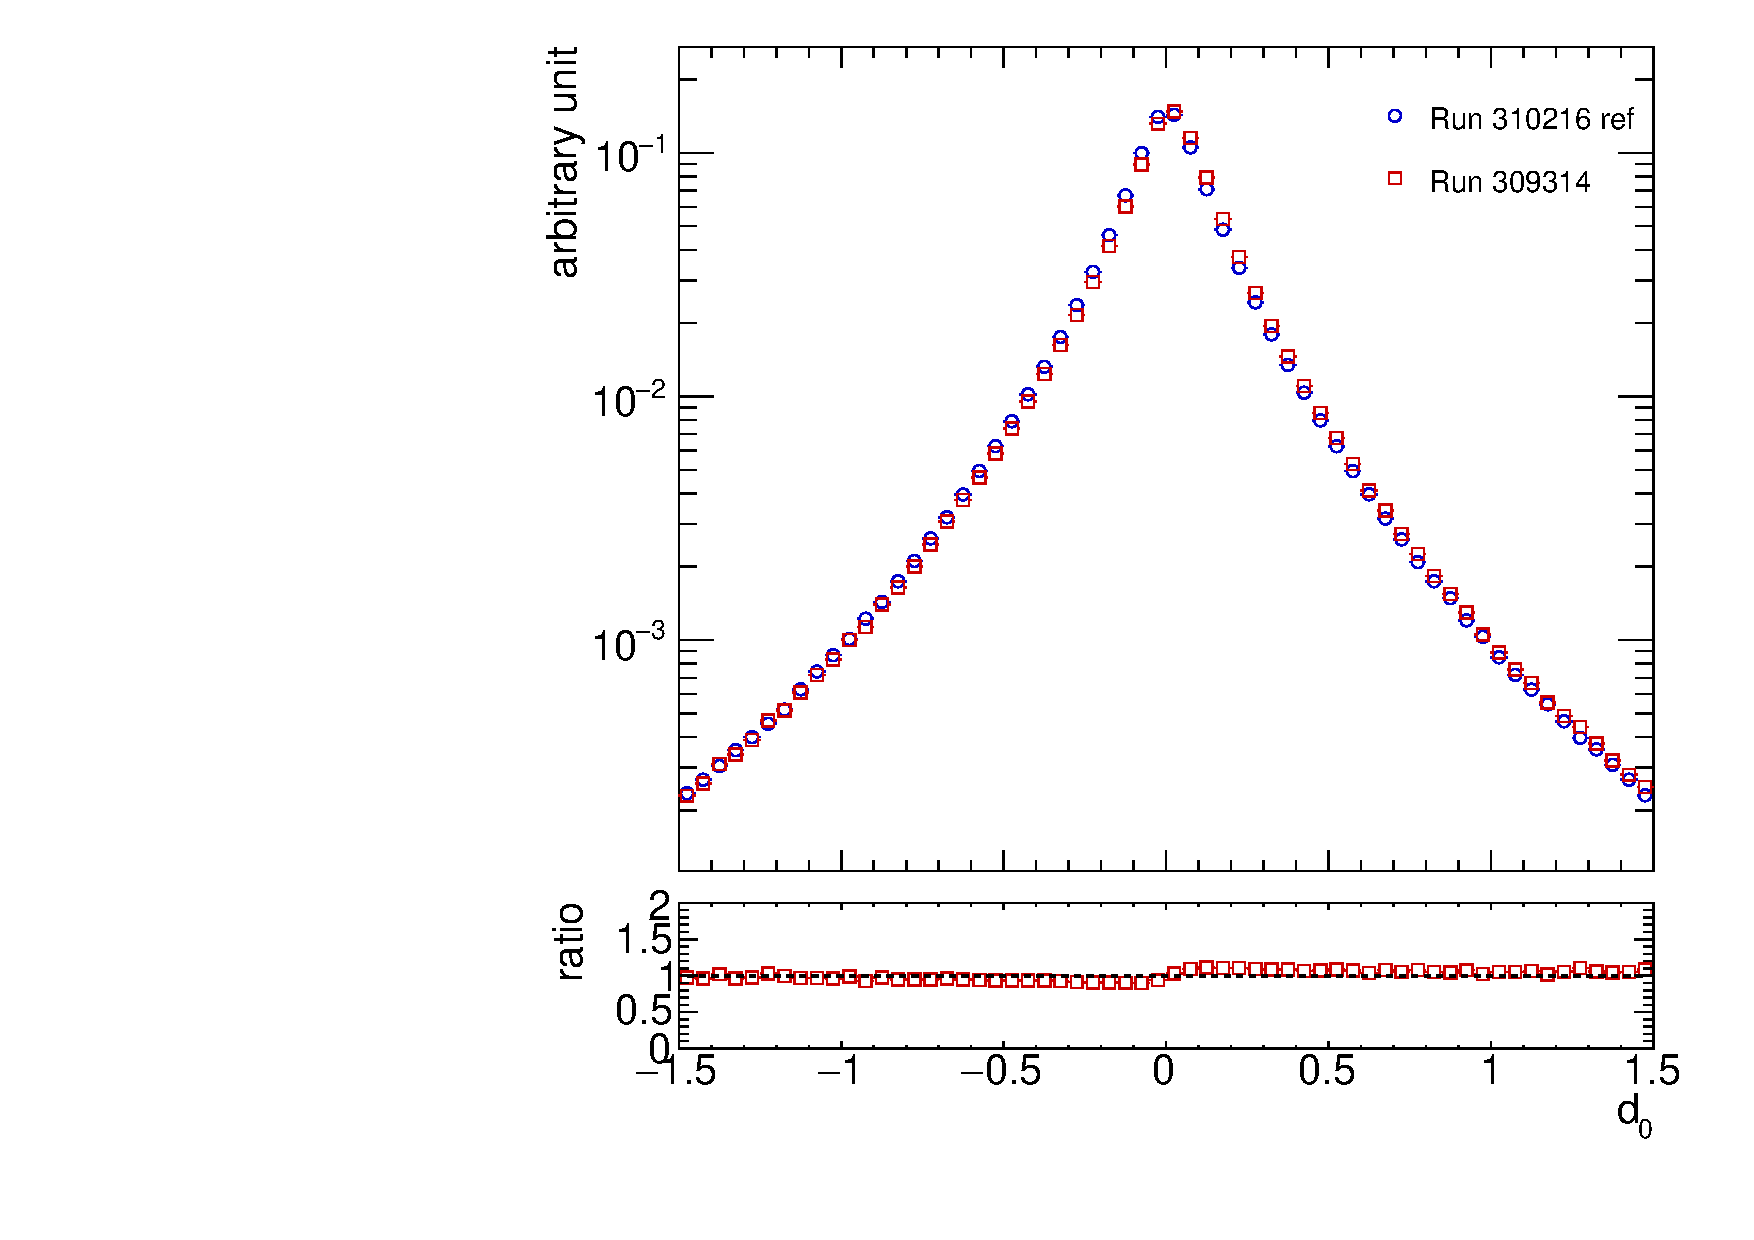
\includegraphics[width=0.45\linewidth]{figs/sec_evtSlc/GRLpp2016/309314_dis_d0.pdf}
\caption{Distribution of $z_{0}\text{sin}\theta$ and $d_{0}$ of reconstructed tracks: a comparison between run 309314 and run 310216.}
\label{fig:GRLpp2016_309314_z0_d0}
\end{figure}
Fig.~\ref{fig:GRLpp2016_309314_z0_d0} shows the comparison of $z_{0}\text{sin}\theta$ and $d_{0}$ distribution of reconstructed tracks, between run 309314 and 310216. They are very consistent.

\begin{figure}[H]
\centering
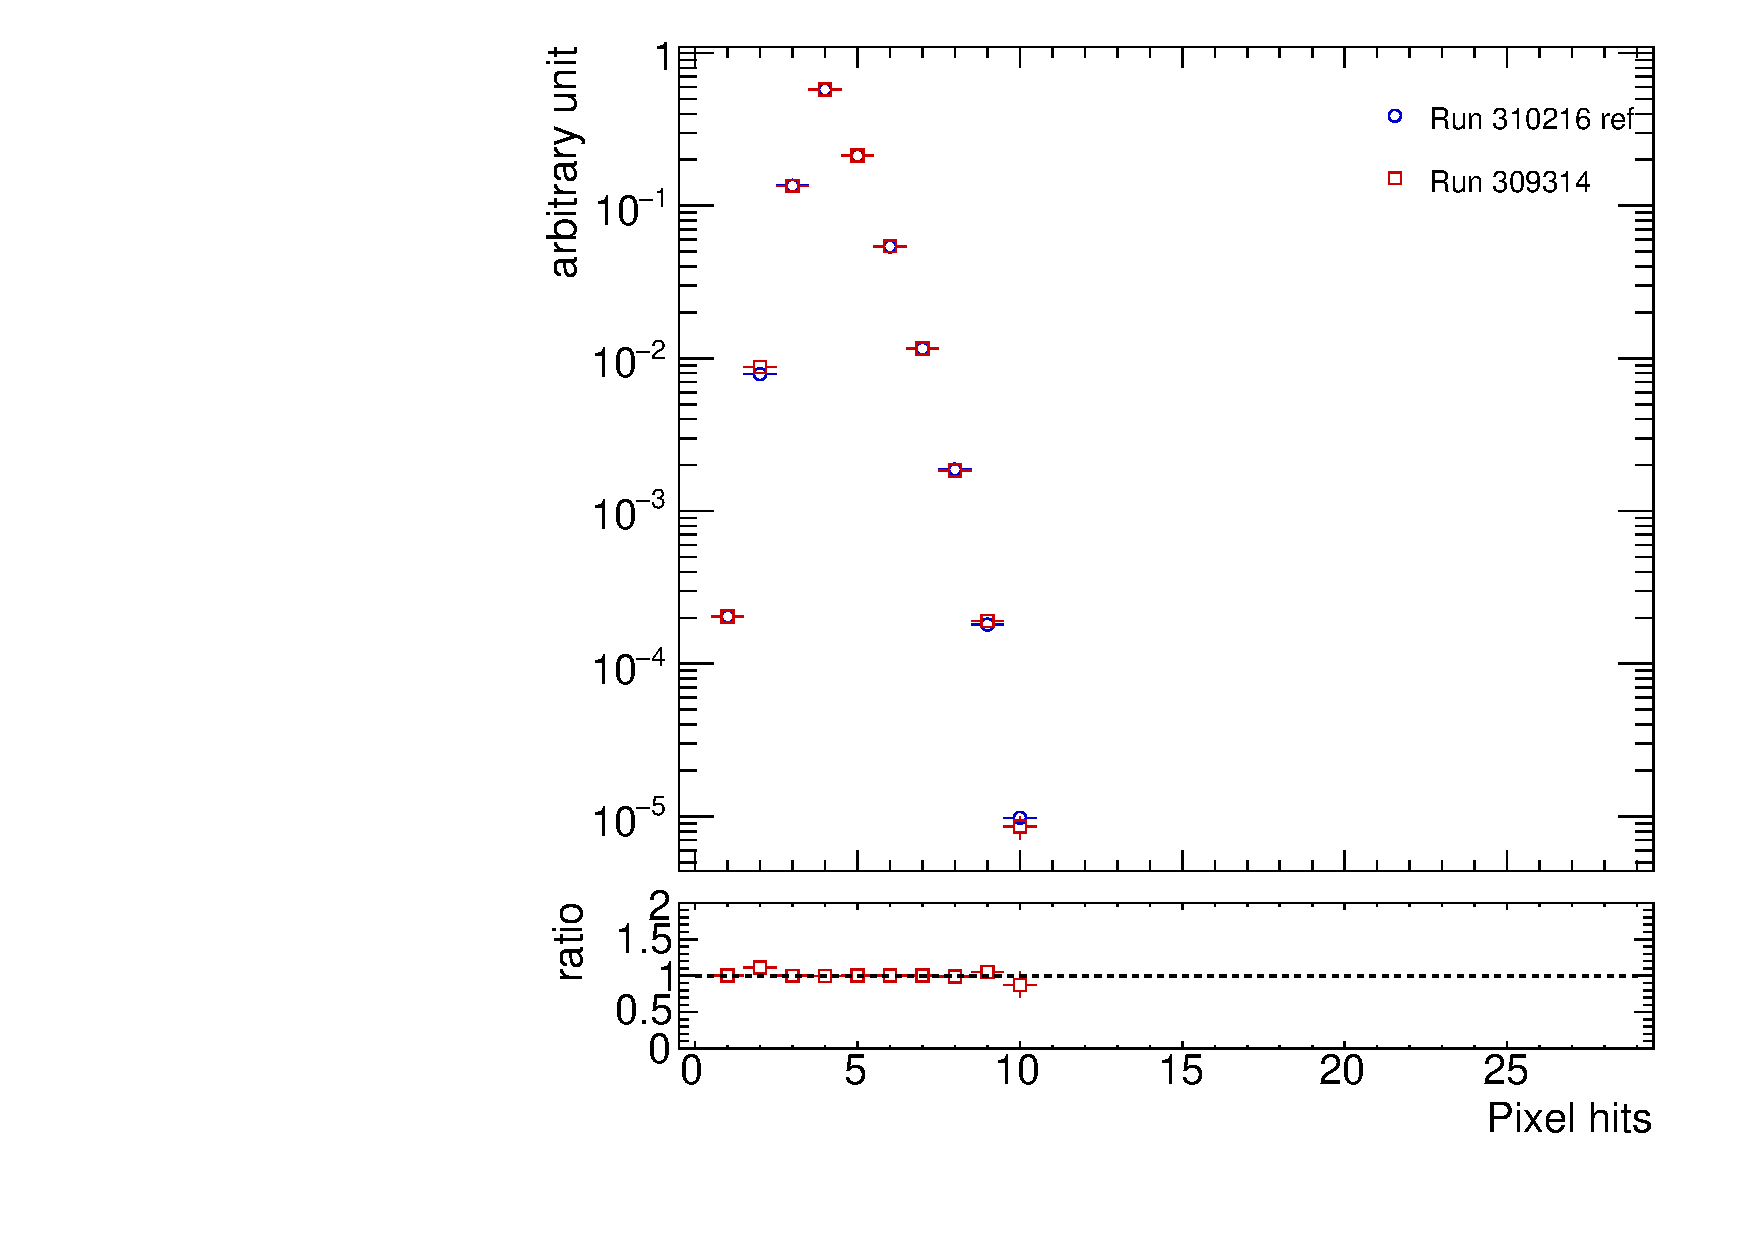
\includegraphics[width=0.45\linewidth]{figs/sec_evtSlc/GRLpp2016/309314_dis_pixHit.pdf}
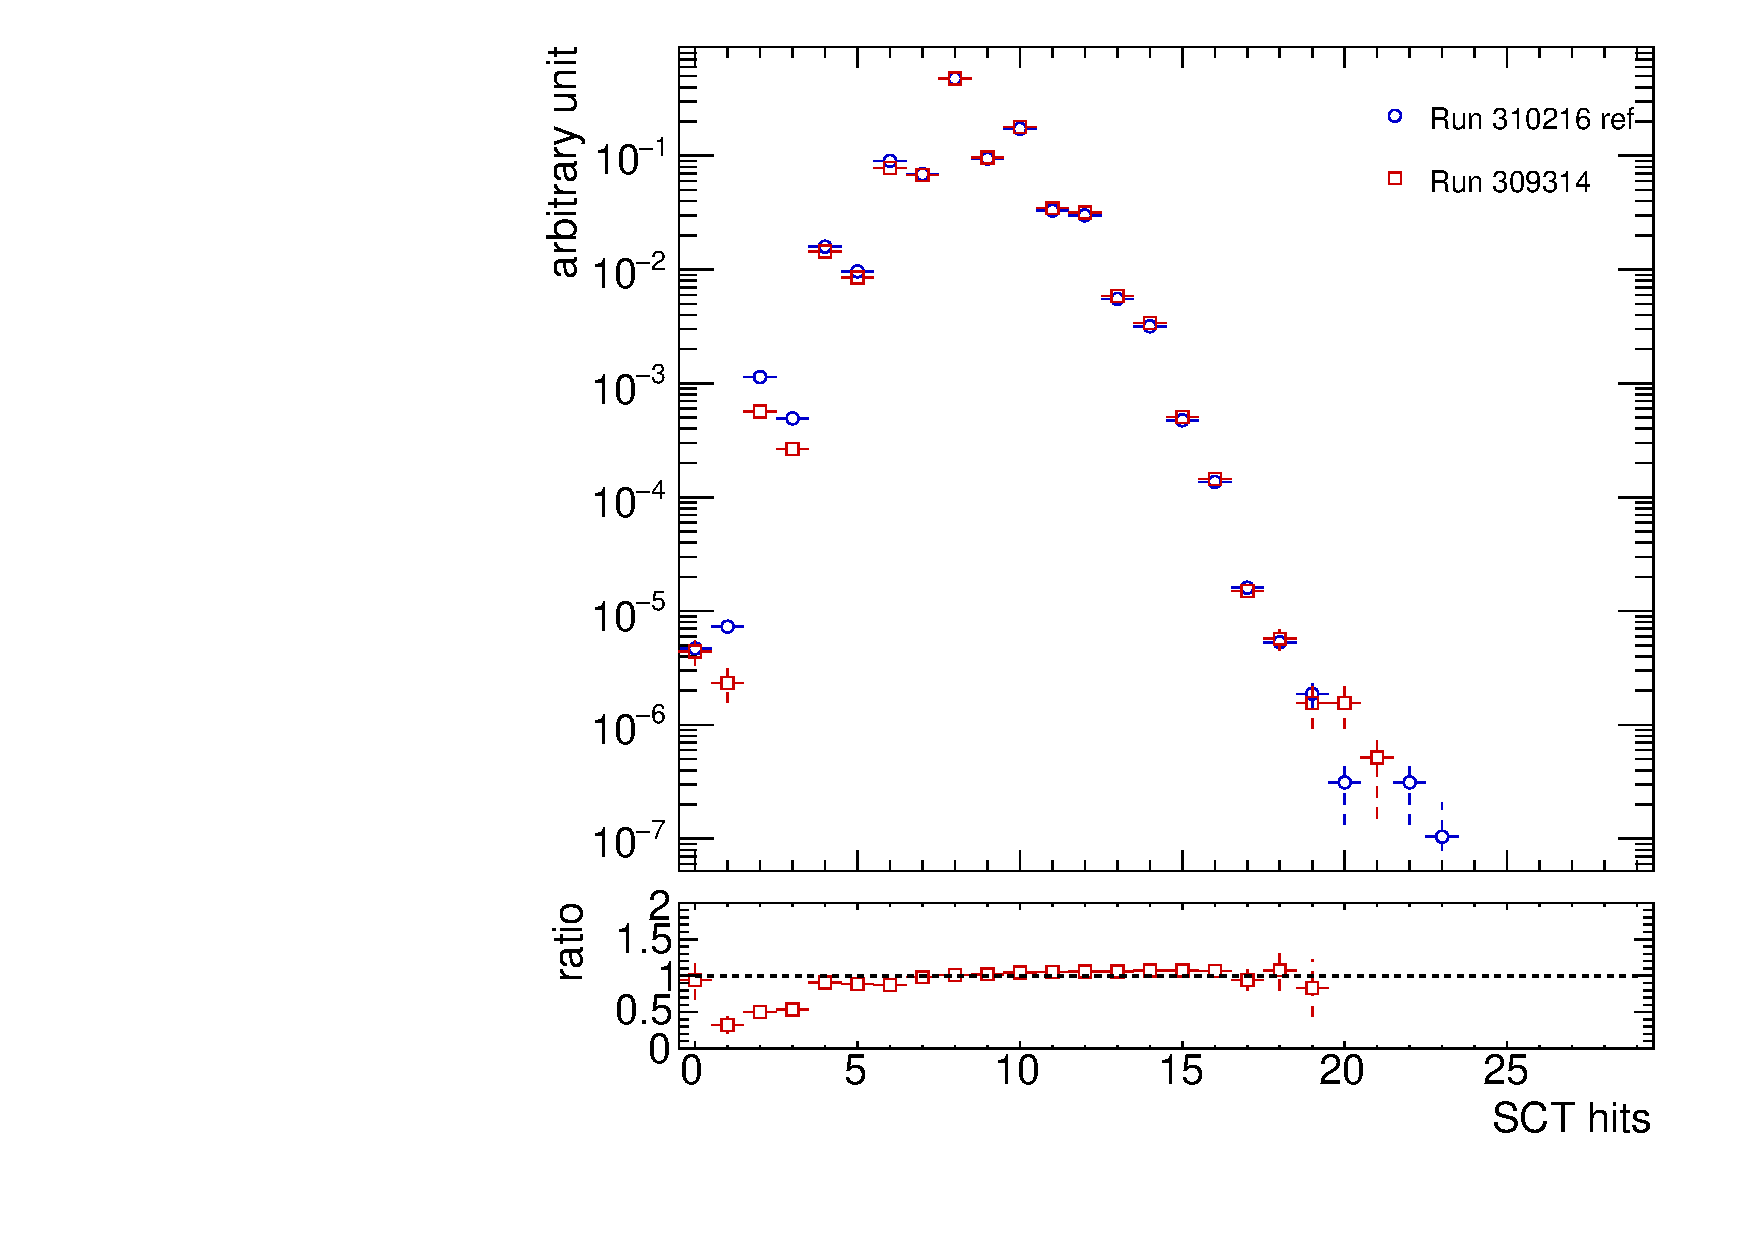
\includegraphics[width=0.45\linewidth]{figs/sec_evtSlc/GRLpp2016/309314_dis_sctHit.pdf}
\caption{Distribution of number of Pixel and SCT hits of reconstructed tracks: a comparison between run 309314 and run 310216.}
\label{fig:GRLpp2016_309314_pixHit_sctHit}
\end{figure}
Fig.~\ref{fig:GRLpp2016_309314_pixHit_sctHit} shows the comparison of number of Pixel and SCT hits, between run 309314 and 310216. They are very consistent.

\begin{figure}[H]
\centering
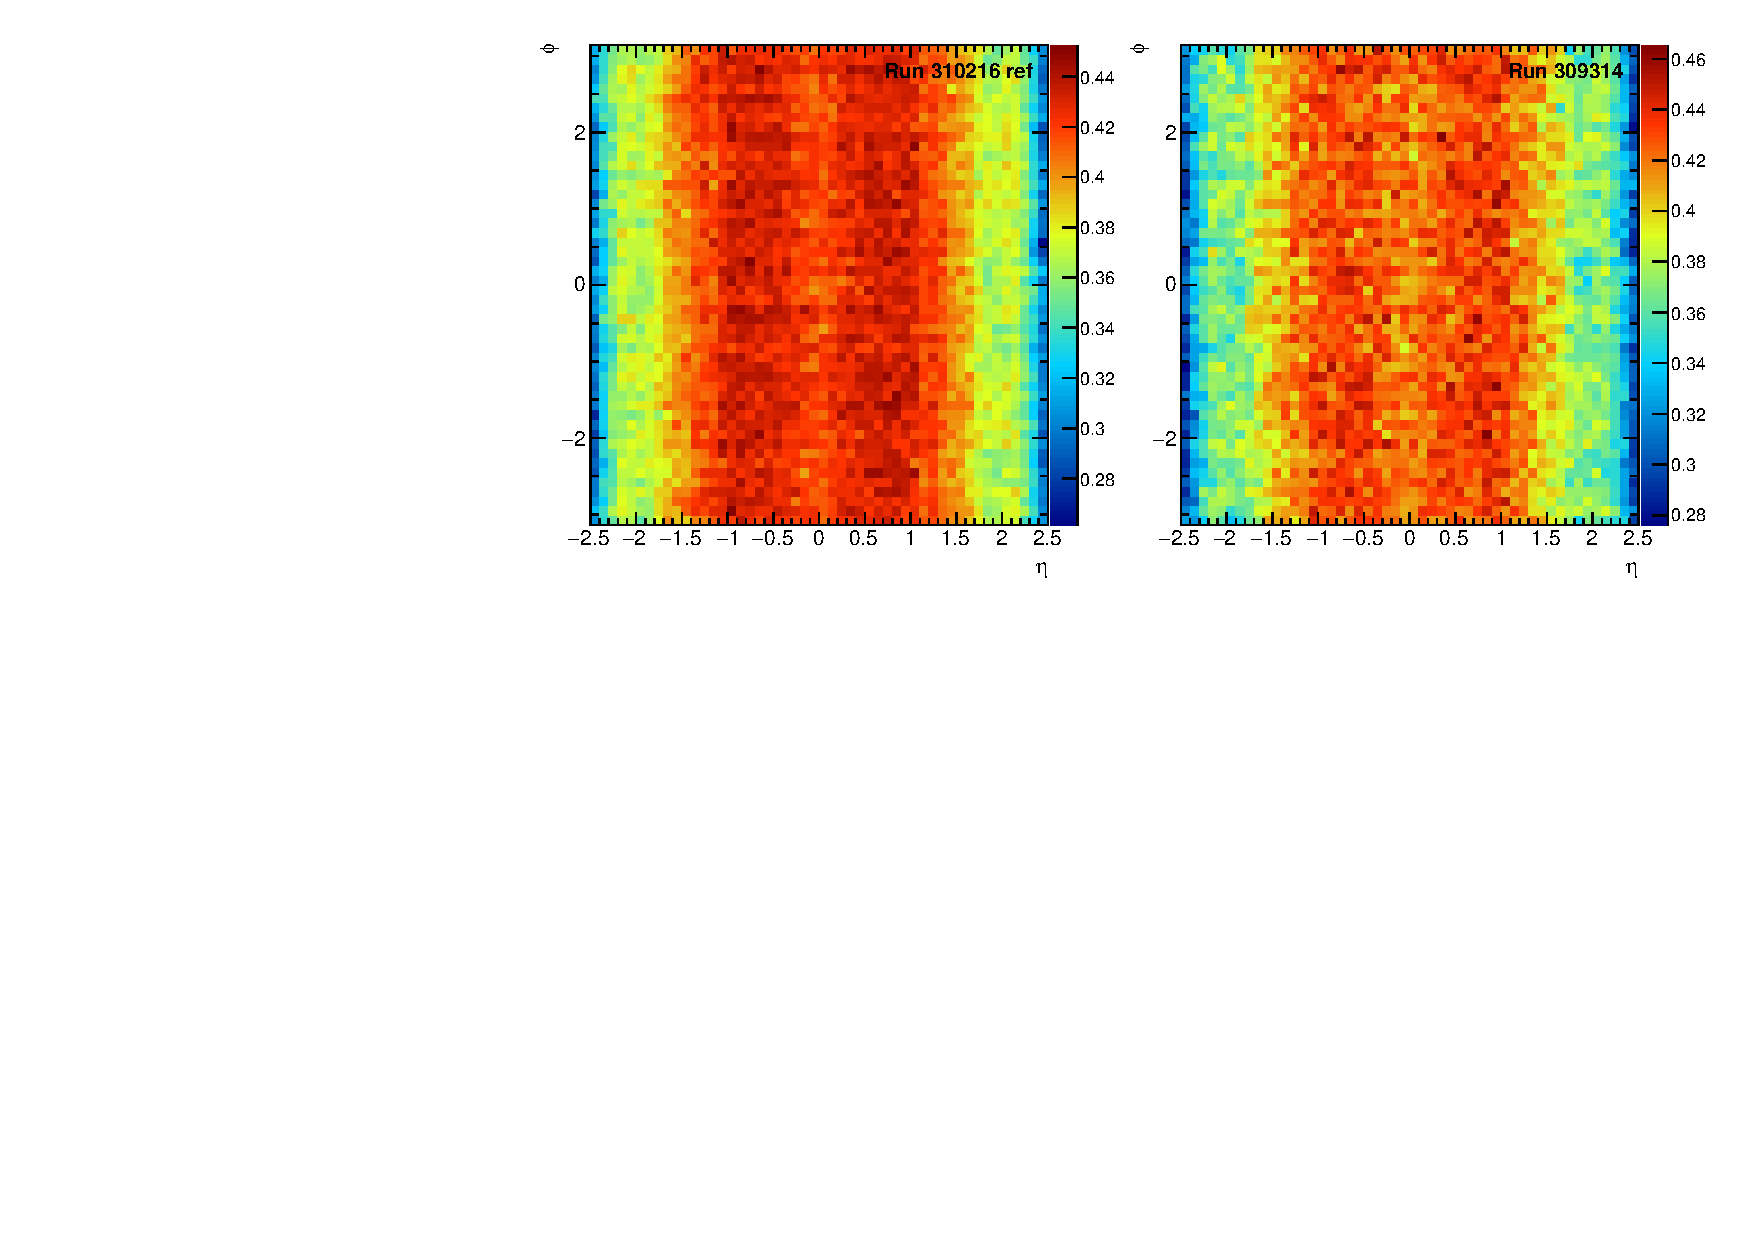
\includegraphics[width=0.9\linewidth]{figs/sec_evtSlc/GRLpp2016/309314_crr_eta_phi.pdf}
\caption{2D map of raw $\eta$-$\phi$ distribution: a comparison between run 309314 and run 310216.}
\label{fig:GRLpp2016_309314_eta_phi}
\end{figure}
Finally, fig.~\ref{fig:GRLpp2016_309314_eta_phi} shows the 2D map of raw $\eta$-$\phi$ distribution. "raw" means the tracks are not weighted by tracking efficiency. The distributions are very consistent.

As a conclusion, even though beam spot is not constraint in these two runs, various tracking quantities are very consistent with the reference run. Due to these reasons, we will include these two runs into the $pp$ analysis.




\subsection{$pp$ 5.02 TeV}
In 2015 before the Pb+Pb run, low-$\mu$ and intermediate-$\mu$ 5.02 TeV $pp$ data was collected with ATLAS detectors. Since this reference run is right after previous $pp$ runs, the track selection is identical to 13 TeV $pp$. All the runs, with GRL selection, are included in this analysis and they are listed as below:
\begin{itemize}

\item Run 286282, peak $\mu=0.58$, 37.3 million events from MinBias stream
\begin{itemize}[leftmargin=*]
\item[] \verb|data15_5TeV.00286282.physics_MinBias.recon.AOD.r7744/|
\end{itemize}

\item Run 286328, peak $\mu=1.58$, 5.8 million events from MinBias stream
\begin{itemize}[leftmargin=*]
\item[] \verb|data15_5TeV.00286328.physics_MinBias.recon.AOD.r7744/|
\end{itemize}

\item Run 286361, peak $\mu=1.34$, 3.5 million events from MinBias stream
\begin{itemize}[leftmargin=*]
\item[] \verb|data15_5TeV.00286361.physics_MinBias.recon.AOD.r7744/|
\end{itemize}

\item Run 286364, peak $\mu=1.58$, 7.9 million events from MinBias stream
\begin{itemize}[leftmargin=*]
\item[] \verb|data15_5TeV.00286364.physics_MinBias.recon.AOD.r7744/|
\end{itemize}

\item Run 286367, peak $\mu=0.67$, 1.7 million events from MinBias stream
\begin{itemize}[leftmargin=*]
\item[] \verb|data15_5TeV.00286367.physics_MinBias.recon.AOD.r7744/|
\end{itemize}

\item Run 286411, peak $\mu=1.33$, 10.8 million events from MinBias stream
\begin{itemize}[leftmargin=*]
\item[] \verb|data15_5TeV.00286411.physics_MinBias.recon.AOD.r7744/|
\end{itemize}

\item Run 286474, peak $\mu=1.25$, 5.3 million events from MinBias stream
\begin{itemize}[leftmargin=*]
\item[] \verb|data15_5TeV.00286474.physics_MinBias.recon.AOD.r7744/|
\end{itemize}

\end{itemize}

Similar as 13 TeV $pp$, the triggers applied in 5 TeV $pp$ have two components: MinBias and HMT. A list of all the major MinBias and HMT triggers used in this analysis is summarized as follows:
\begin{itemize}
\item \verb|HLT_mb_sptrk|
\item \verb|HLT_noalg_mb_L1MBTS_1|
\item \verb|HLT_mb_sp800_pusup400_trk50_hmt_L1TE5|
\item \verb|HLT_mb_sp900_pusup500_trk60_hmt_L1TE5|
\item \verb|HLT_mb_sp1200_pusup700_trk70_hmt_L1TE5|
\item \verb|HLT_mb_sp1400_pusup550_trk90_hmt_L1TE10|
\end{itemize}
where a new trigger item has been introduced:
\begin{itemize}
\item \verb|pusup|: maximum number of hits from a vertex, used to suppress pile-up events before track reconstruction;
\end{itemize}

\begin{figure}[H]
\centering
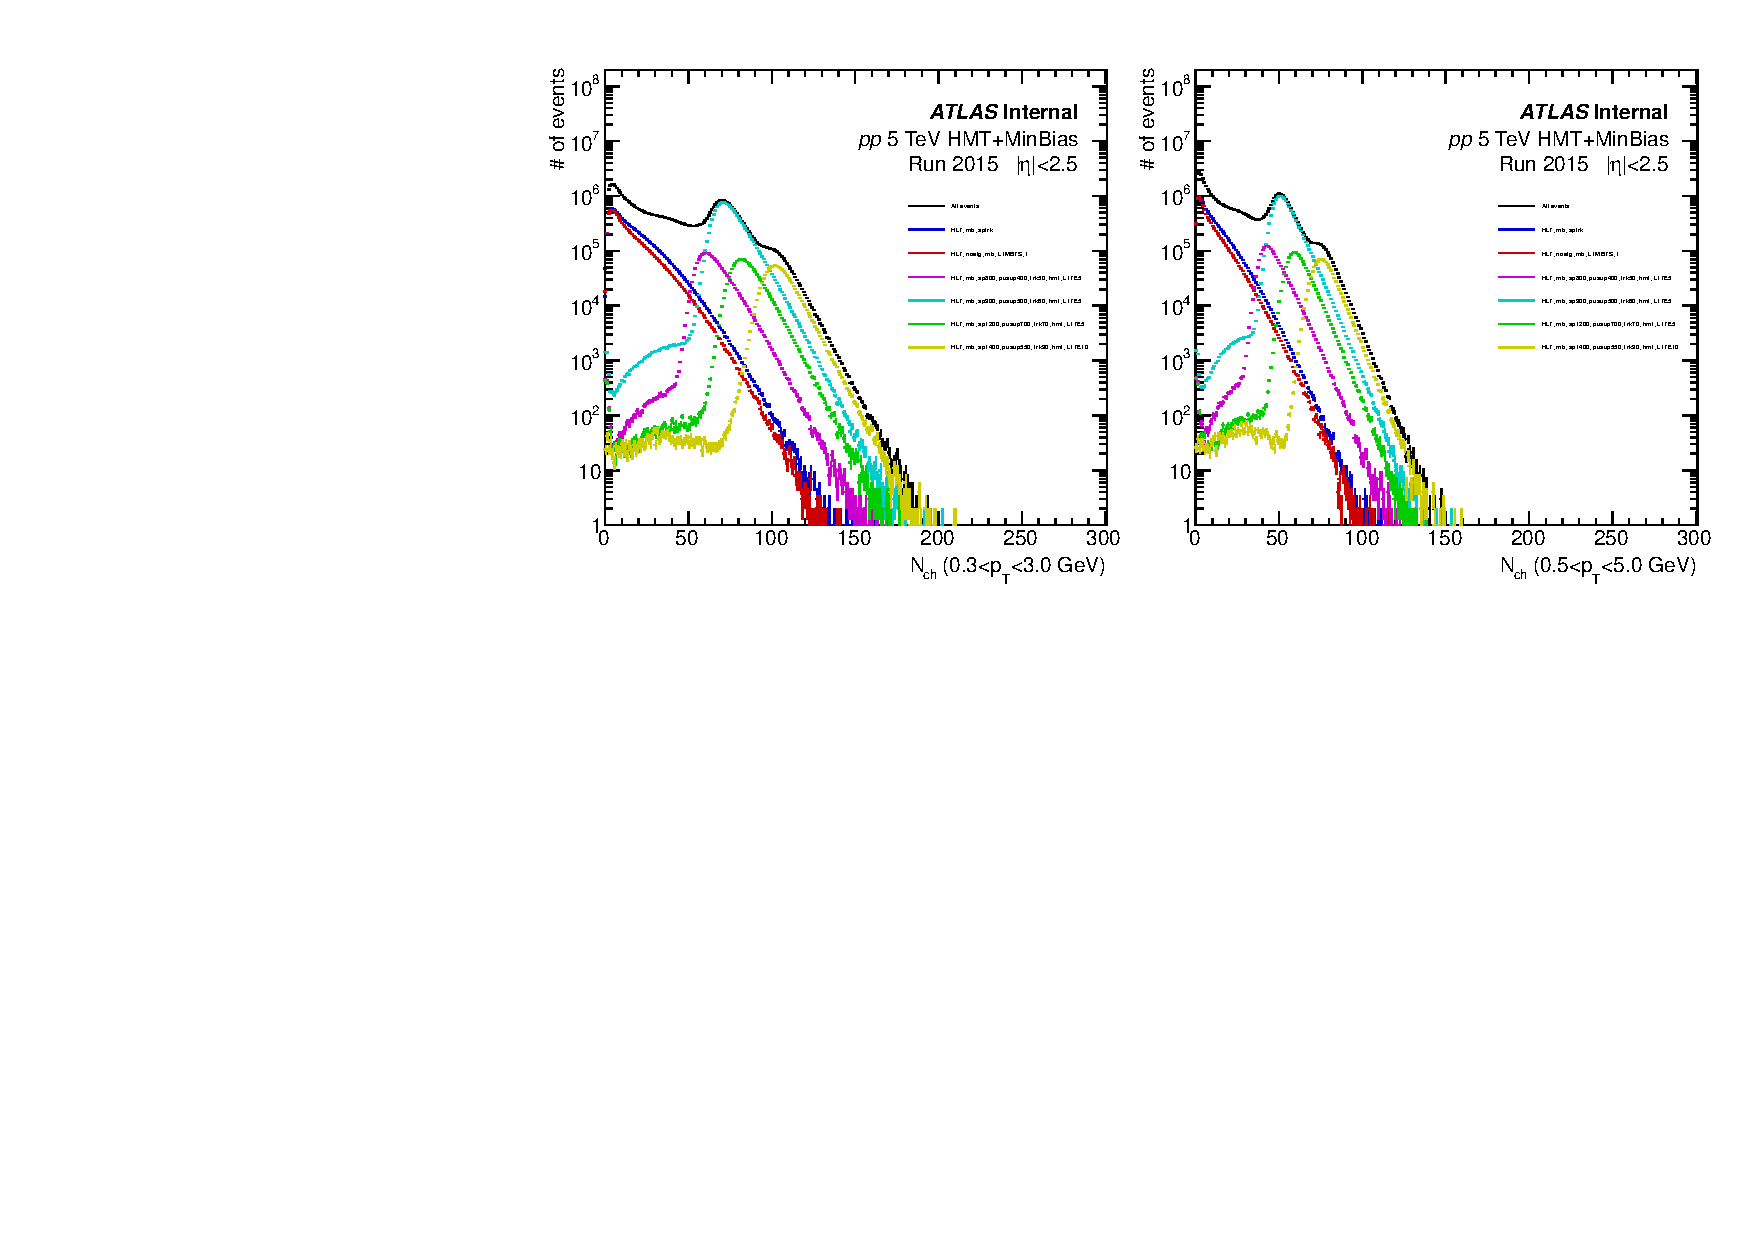
\includegraphics[width=.9\linewidth]{figs/sec_evtSlc/trkDis_pp5.pdf}
\caption{Distribution of number of tracks with two $p_{T}$ thresholds: $0.3<p_{T}<3.0$ GeV and $0.5<p_{T}<5.0$ GeV, in 13 TeV $pp$ run period 4. The major MinBias and HMT triggers are plotted separately.}
\label{fig:trkDis_pp5}
\end{figure}
The summary of statistics with all the major triggers used in this analysis are shown in Fig.~\ref{fig:trkDis_pp5}.

\begin{figure}[H]
\centering
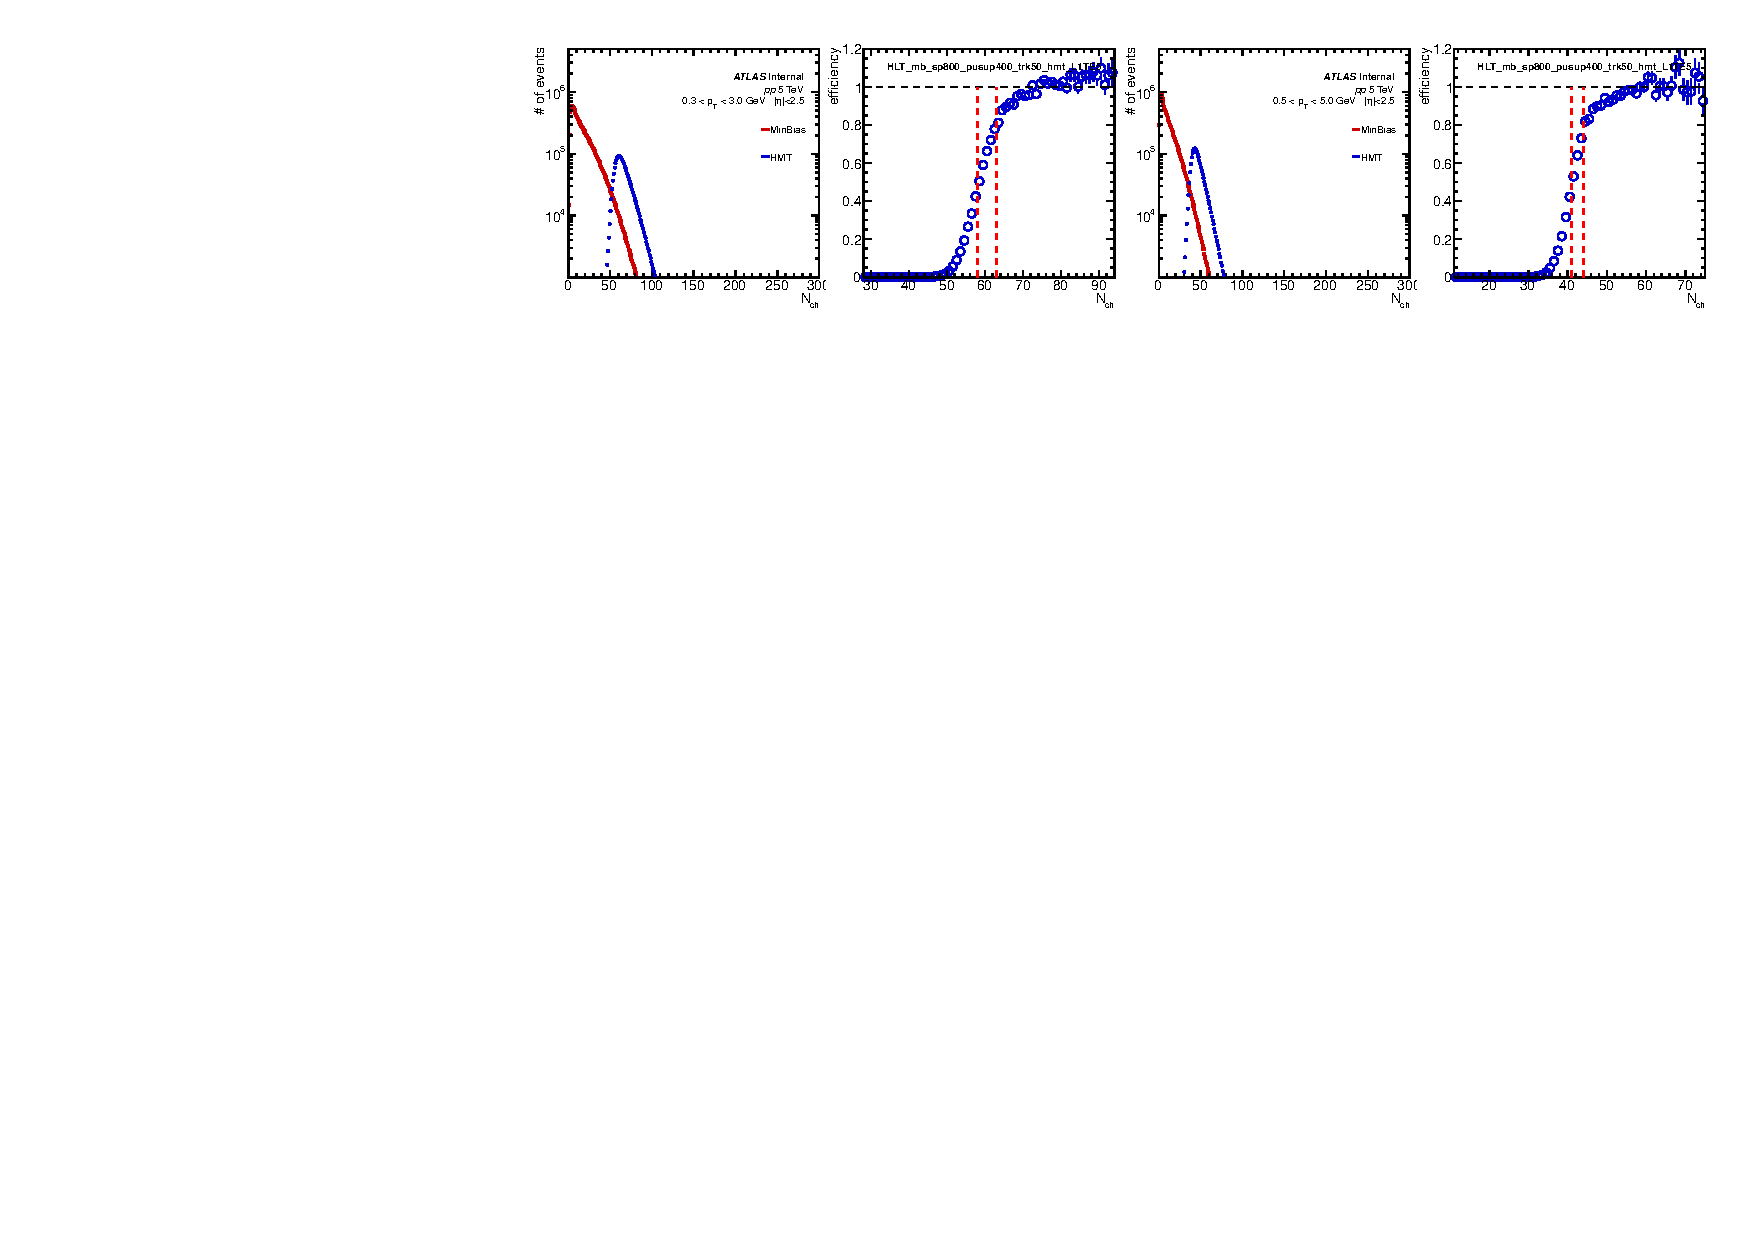
\includegraphics[width=1.\linewidth]{figs/sec_evtSlc/trigEff_pp5/trigEff_Trig18.pdf}
\end{figure}
\begin{figure}[H]
\centering
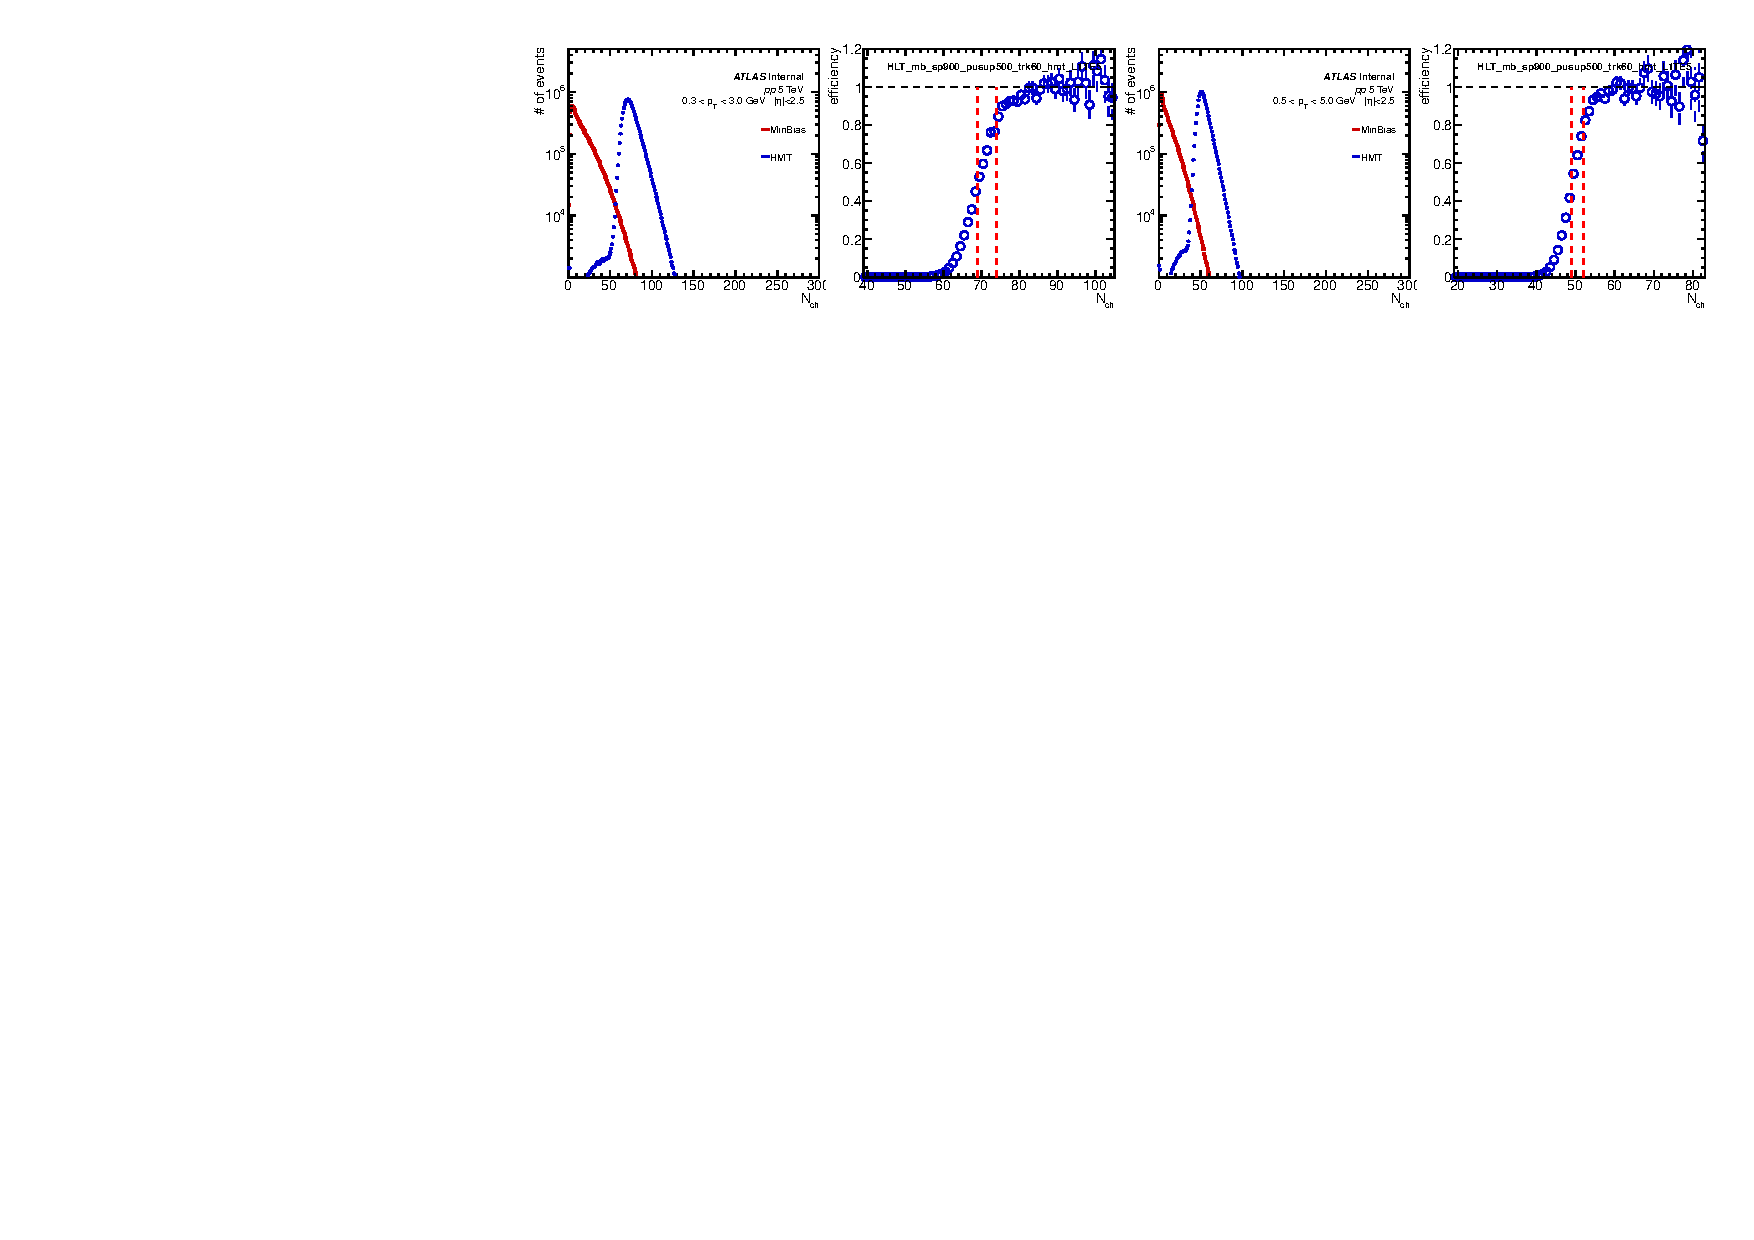
\includegraphics[width=1.\linewidth]{figs/sec_evtSlc/trigEff_pp5/trigEff_Trig19.pdf}
\end{figure}
\begin{figure}[H]
\centering
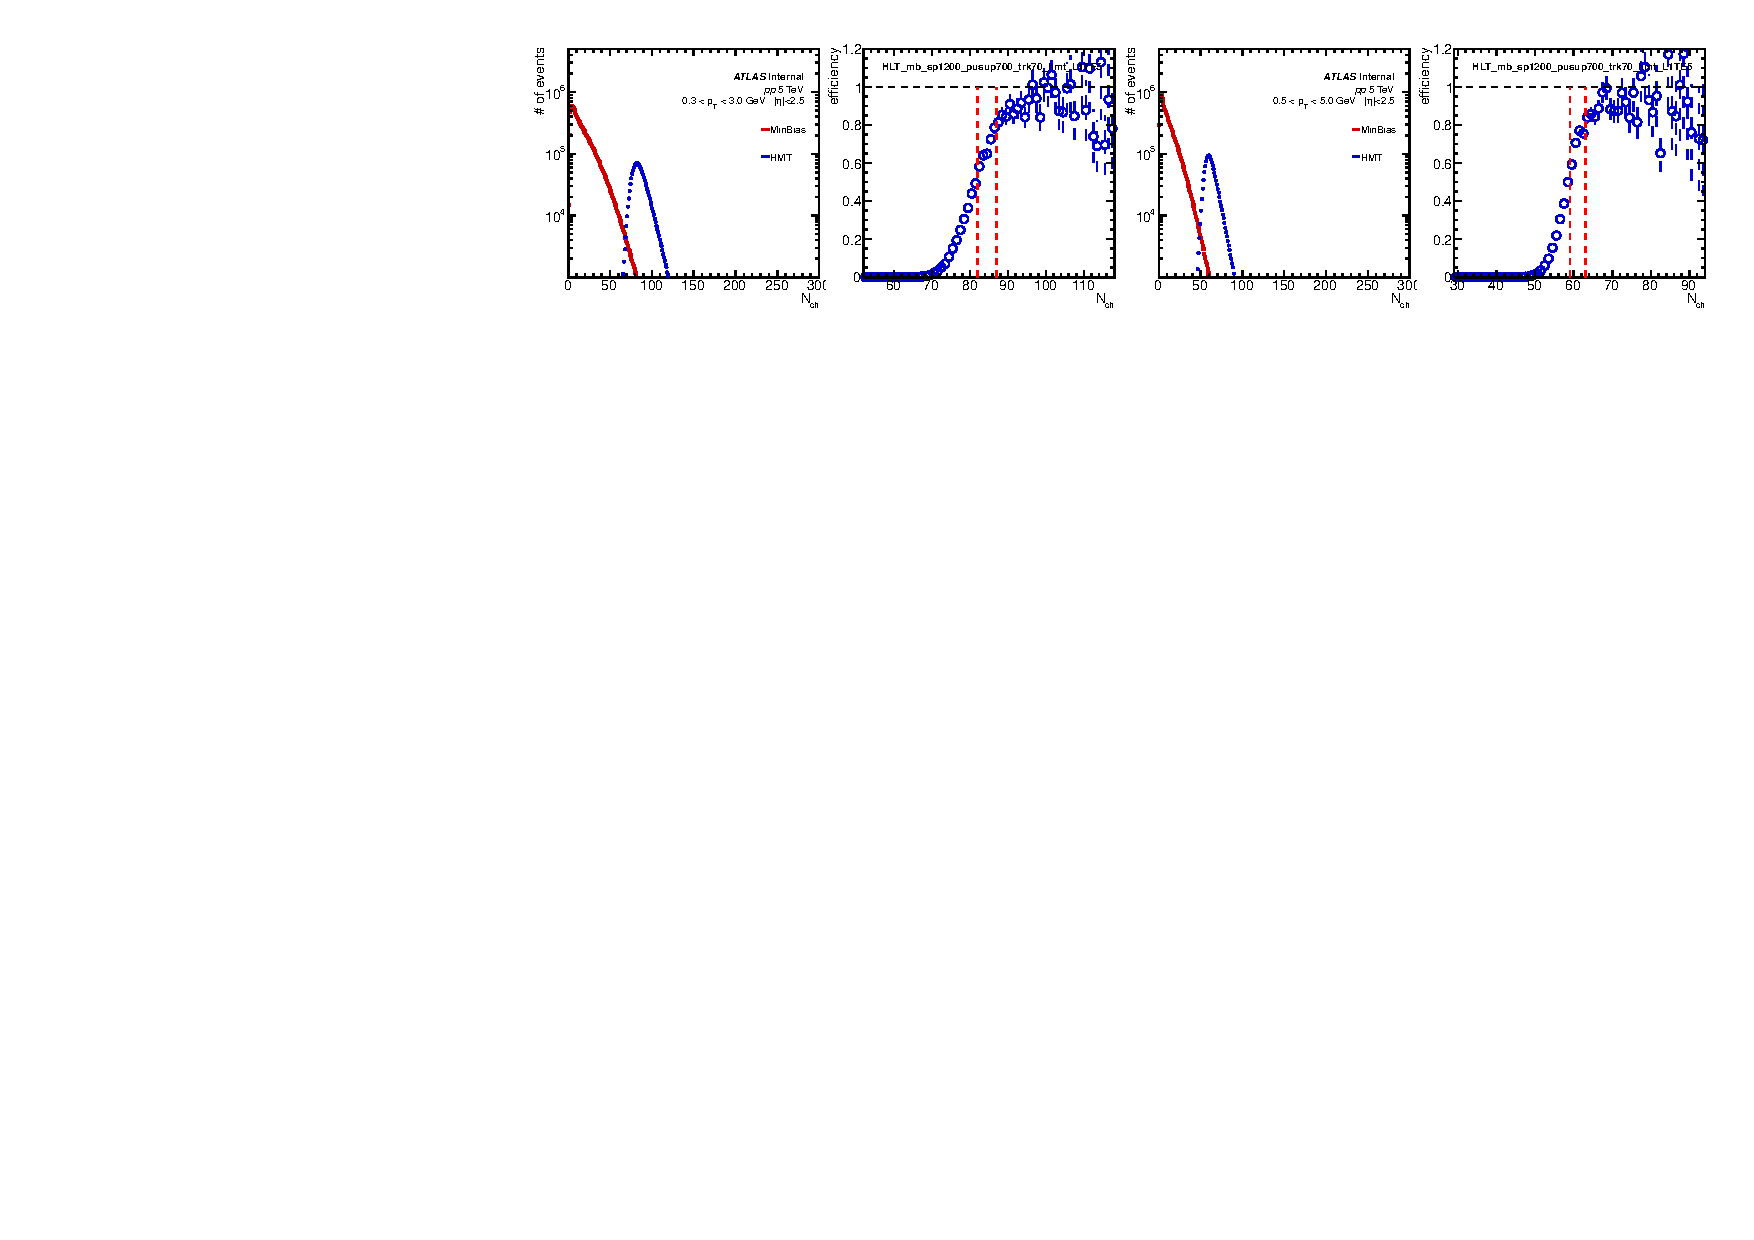
\includegraphics[width=1.\linewidth]{figs/sec_evtSlc/trigEff_pp5/trigEff_Trig20.pdf}
\end{figure}
\begin{figure}[H]
\centering
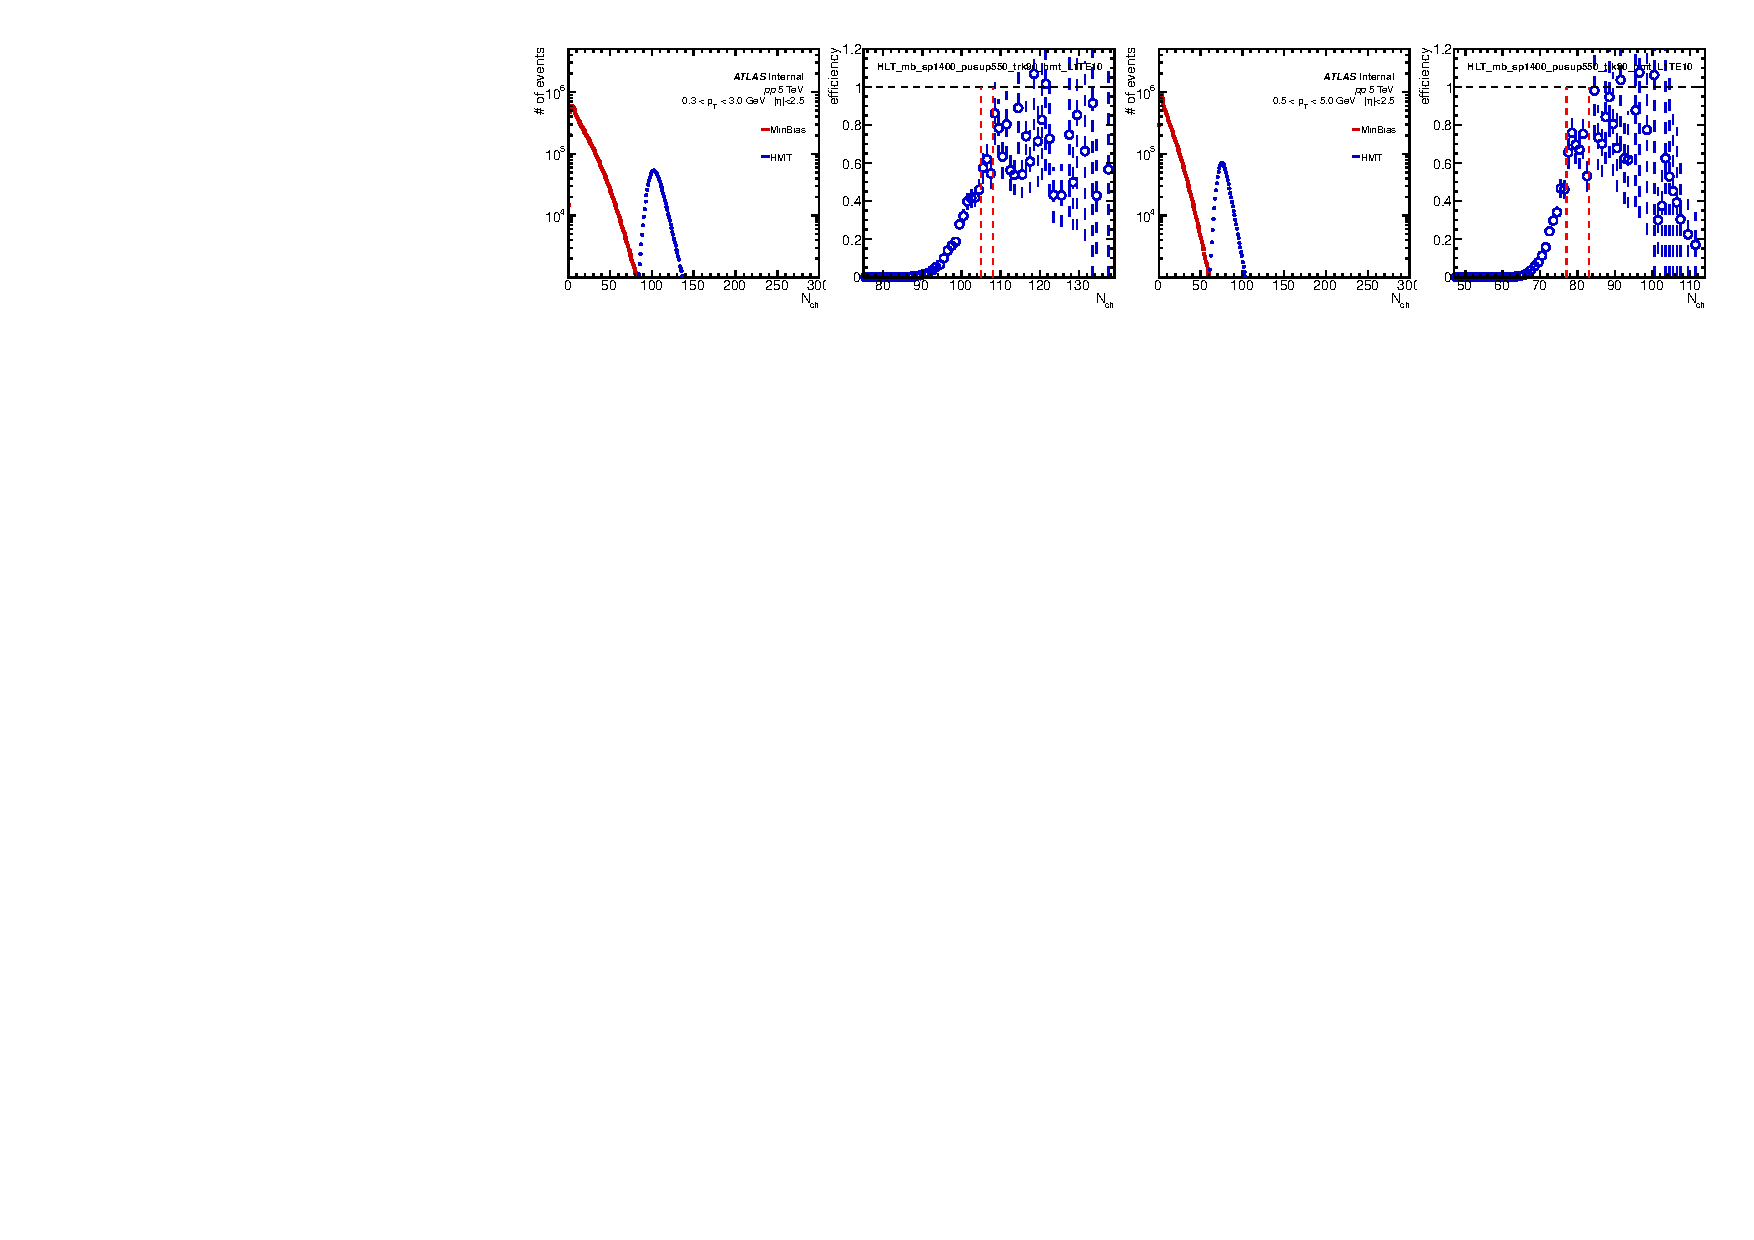
\includegraphics[width=1.\linewidth]{figs/sec_evtSlc/trigEff_pp5/trigEff_Trig21.pdf}
\caption{Trigger efficiencies of all major HMT triggers as a function of number of tracks in two $p_{T}$ ranges: $0.3<p_{T}<3.0$ GeV and $0.5<p_{T}<5.0$ GeV, from 5 TeV $pp$ run. Efficiency is calculated relative to the corresponding MinBias trigger in this run period then scaled to 1.0 in the large $N_{ch}$ region. The two red dash lines indicate 50$\%$ and 80$\%$ efficiency cuts.}
\label{fig:trigEff_pp5}
\end{figure}
Trigger efficiencies of all the major HMT triggers are summarized in Fig.~\ref{fig:trigEff_pp5}, where efficiencies are shown for two $p_{T}$ ranges separately: $0.3<p_{T}<3.0$ GeV and $0.5<p_{T}<5.0$ GeV.

\subsubsection{PYTHIA for $pp$ 5.02 TeV data}
Since the 5 TeV $pp$ run is close to 13 TeV run in time, the detector effects between the two runs should be similar. For his reason, tracking efficiency and fraction of fake tracks extracted from 13 TeV PYTHIA is applied to 5 TeV $pp$ data.

\subsubsection{Impact of ID misalignment}
In order to study the effect of ID misalignment, the package \verb|InDetTrackSystema9csTools-00-00-18| was used. The 5 TeV $pp$ cumulant are recalculated with the corrected track momenta and compared to the default measurement.

\begin{figure}
\centering
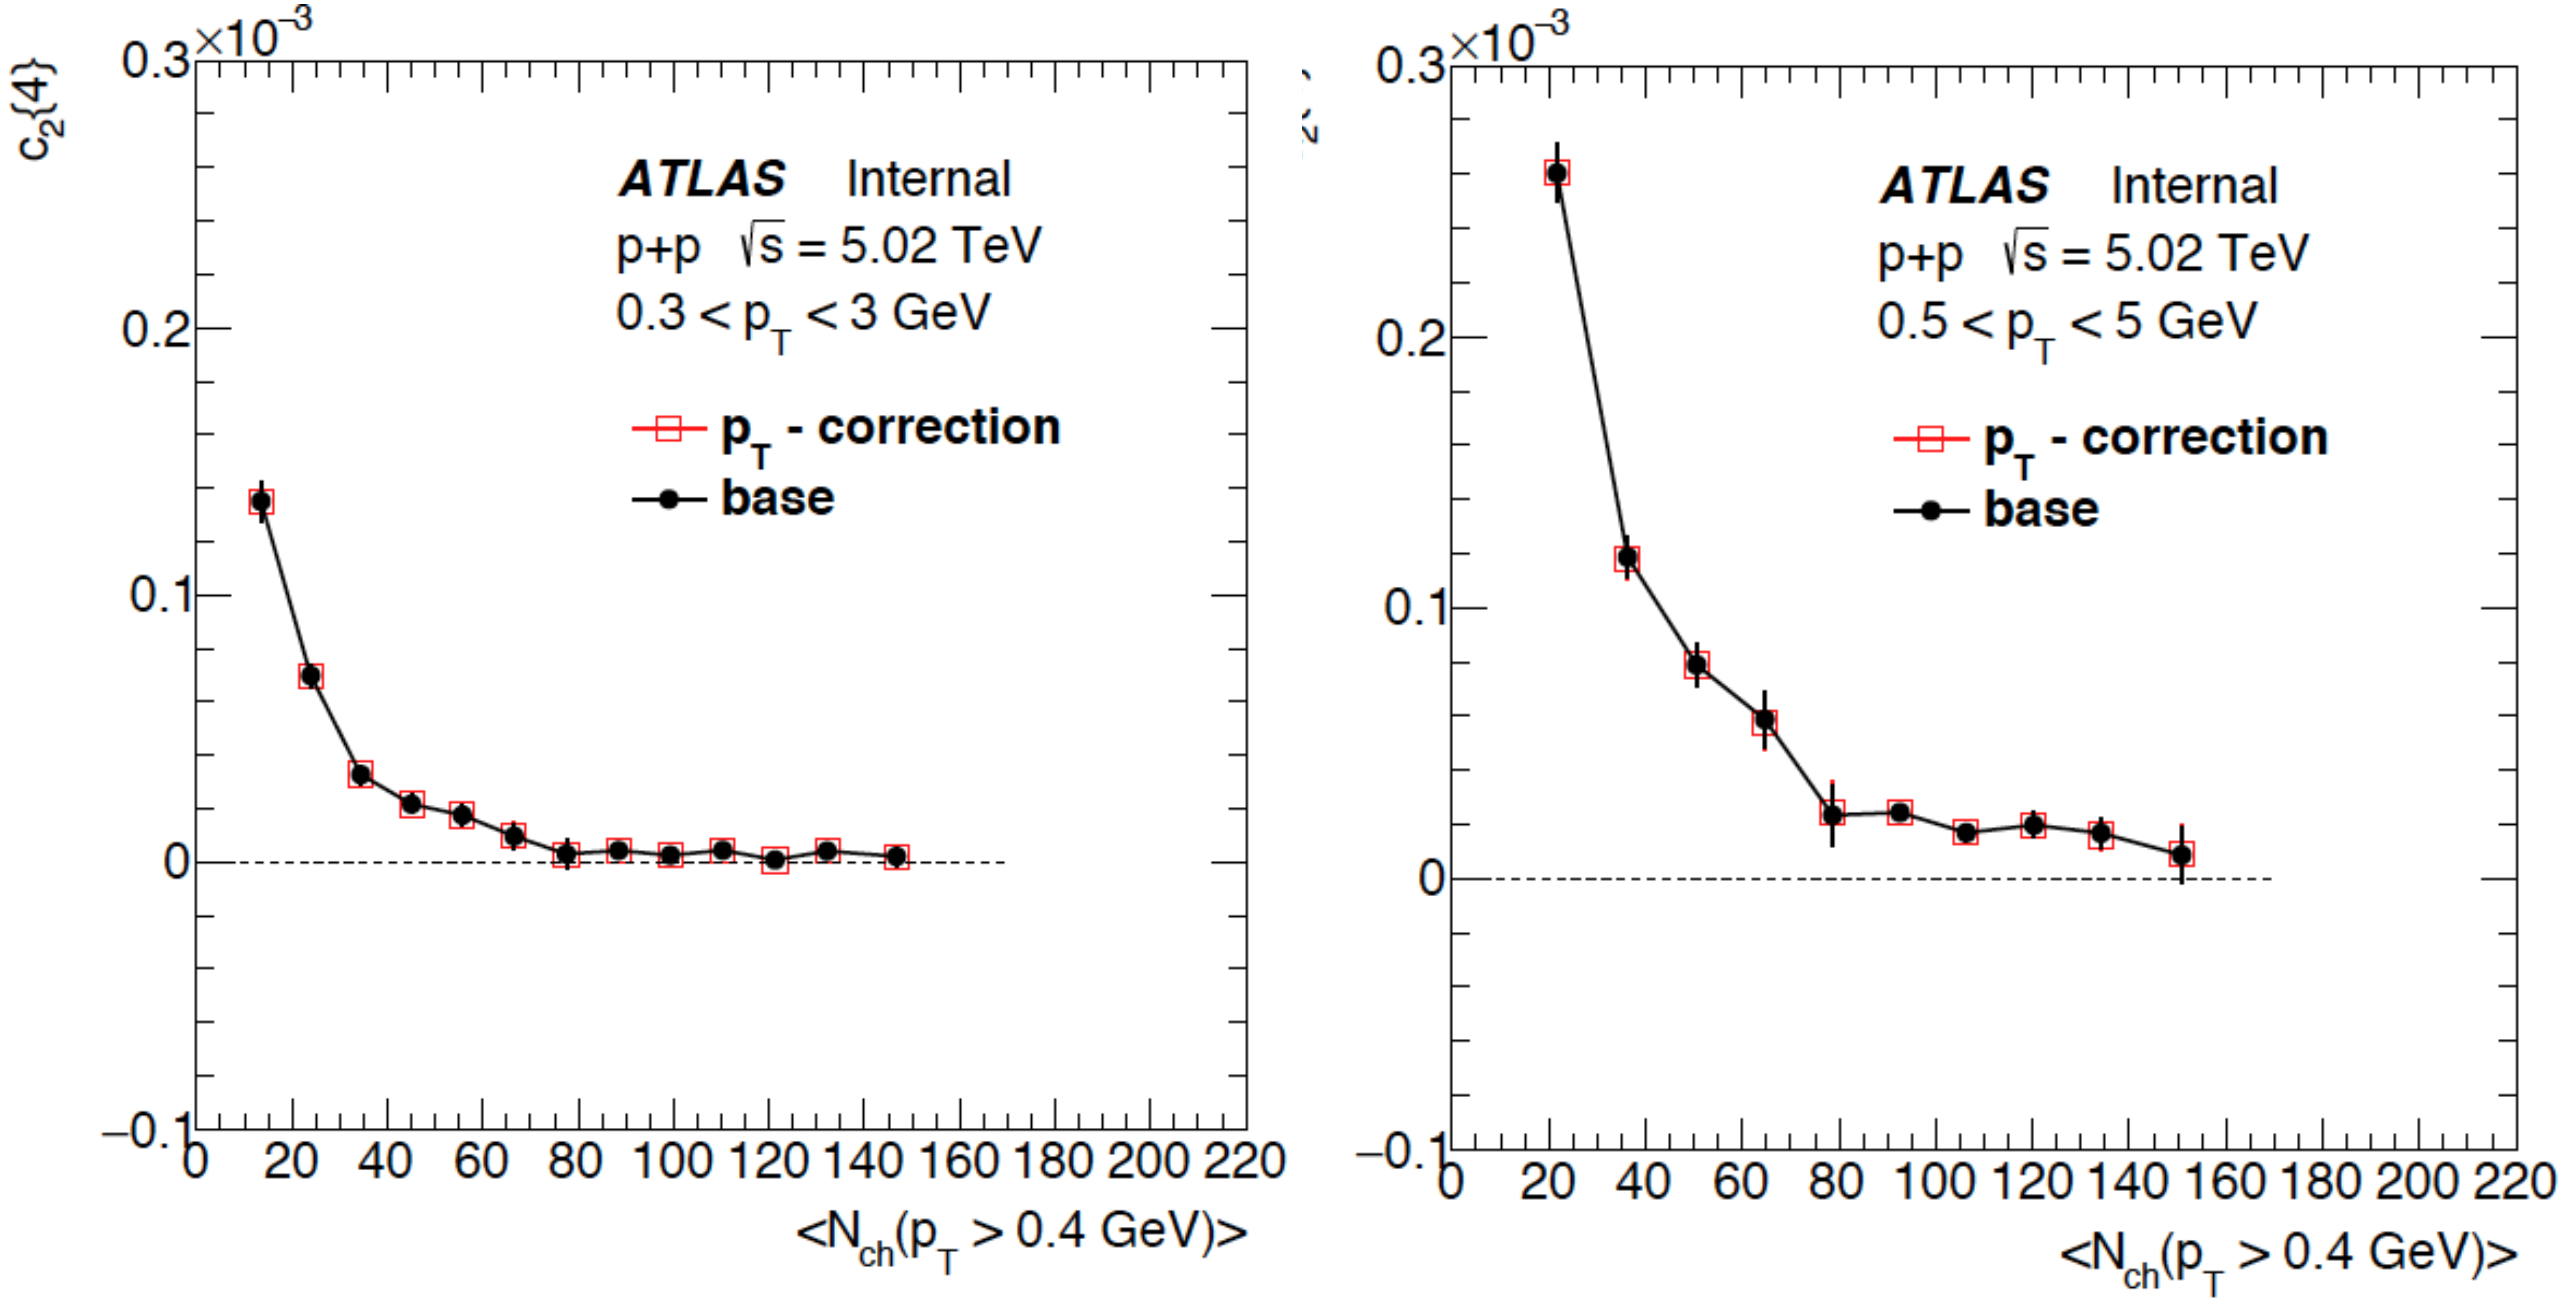
\includegraphics[width=1.\linewidth]{figs/sec_evtSlc/ID_alignment_pp5.png}
\caption{$c_{2}{4}$ measured with default and $p_{\text{T}}$ corrected, for $0.3<p_{\text{T}}<3.0$ GeV (left) and $0.5<p_{\text{T}}<5.0$ GeV (right).}
\label{fig:ID_alignment_pp5}
\end{figure}
For $c_{2}{4}$ the effects of ID misalignment for low multiplicity (up to 60) is at $0.1\%$ level. At higher multiplicity the difference is smaller than statistical errors. This concludes that the ID misalignment has minimal impact on this analysis.

\subsection{$p$+Pb 5.02 TeV}
5.02 TeV $p$+Pb data have been collected in 2013~\cite{Aad:2012bu} and 2016. Since the event and tracking selections are quite different between Run 1 and Run 2, they will be discussed separately in the following sections.

\subsubsection{2013 $p$+Pb}
In 2013, low-$\mu$ 5.02 TeV $p$+Pb data was collected with ATLAS detectors. In additional to GRL selection, each event also needs to pass the MBTS cuts:
\begin{itemize}
\item $|\text{time}_{A}|$ or $|\text{time}_{C}|$ must not equal 75 or 0 ns;
\item $|\text{time}_{A}-\text{time}_{C}|<10$ ns;
\end{itemize}
and the pile-up events are suppressed by rejecting events containing more than one good reconstructed vertex. The remaining pileup events are further suppressed based on the signal in the ZDC on the Pb-fragmentation side. This signal is calibrated to the number of detected neutrons ($N_{n}$) based on the location of the peak corresponding to a single neutron. The distribution of $N_{n}$ in events with pileup is broader than that for the events without pileup. Hence, a simple cut on the high tail end of the ZDC signal distribution further suppresses the pileup, while retaining more than 98$\%$ of the events without pileup. After this pileup rejection procedure, the residual pileup fraction is estimated to be 1$\%$ in the event class with the highest track multiplicity studied in this analysis. For details of this pile-up rejection, refer to the internal note of flow measurements in $p$+Pb~\cite{atlas:9}.

The track selection criteria is $p$+Pb is slightly different from $pp$~\cite{Aad:2015gqa, Aad:2016mok}:
\begin{itemize}
\item Tracks are from primary vertex
\item Present hit in B-Layer if expected
\item At least 1 pixel hit
\item $p_{T}<300$ MeV: at least 4 SCT hits + dead sensors
\item $p_{T}>300$ MeV: at least 6 SCT hits + dead sensors
\item significance of $d_{0}$ is $<3.0$
\item significance of $z_{0}\text{sin}\theta$ is $<3.0$
\item $|\eta|\le 2.5$
\item $p_{T}\ge 200$ MeV
\end{itemize}
In additional, an additional tighter cut defined to be the track selection requirements in Pb-Pb analysis is used to check the stability of results in the systematics section.

All the runs included in this analysis are listed as follows. A special reprocessing was done for these runs so that the lowest $p_{T}$ goes down to 0.1 GeV.

\begin{itemize}

\item Run 217999, 4.7 million events from MinBias stream
\begin{itemize}[leftmargin=*]
\item[] \verb|data13_hip.00217999.physics_MinBias.merge.NTUP_HI.r5813_p1729/|
\end{itemize}

\item Run 218006, 2.7 million events from MinBias stream
\begin{itemize}[leftmargin=*]
\item[] \verb|data13_hip.00218006.physics_MinBias.merge.NTUP_HI.r5813_p1729/|
\end{itemize}

\item Run 218048, 6.6 million events from MinBias stream
\begin{itemize}[leftmargin=*]
\item[] \verb|data13_hip.00218048.physics_MinBias.merge.NTUP_HI.r5813_p1729/|
\end{itemize}

\item Run 218118, 3.9 million events from MinBias stream
\begin{itemize}[leftmargin=*]
\item[] \verb|data13_hip.00218118.physics_MinBias.merge.NTUP_HI.r5813_p1729/|
\end{itemize}

\item Run 218168, 4.2 million events from MinBias stream
\begin{itemize}[leftmargin=*]
\item[] \verb|data13_hip.00218168.physics_MinBias.merge.NTUP_HI.r5813_p1729/|
\end{itemize}

\item Run 218179, 4.5 million events from MinBias stream
\begin{itemize}[leftmargin=*]
\item[] \verb|data13_hip.00218179.physics_MinBias.merge.NTUP_HI.r5813_p1729/|
\end{itemize}

\item Run 218213, 1.8 million events from MinBias stream
\begin{itemize}[leftmargin=*]
\item[] \verb|data13_hip.00218213.physics_MinBias.merge.NTUP_HI.r5813_p1729/|
\end{itemize}

\item Run 218222, 0.5 million events from MinBias stream
\begin{itemize}[leftmargin=*]
\item[] \verb|data13_hip.00218222.physics_MinBias.merge.NTUP_HI.r5813_p1729/|
\end{itemize}

\item Run 218301, 3.8 million events from MinBias stream
\begin{itemize}[leftmargin=*]
\item[] \verb|data13_hip.00218301.physics_MinBias.merge.NTUP_HI.r5813_p1729/|
\end{itemize}

\item Run 218338, 3.8 million events from MinBias stream
\begin{itemize}[leftmargin=*]
\item[] \verb|data13_hip.00218338.physics_MinBias.merge.NTUP_HI.r5813_p1729/|
\end{itemize}

\item Run 218391, 8.0 million events from MinBias stream
\begin{itemize}[leftmargin=*]
\item[] \verb|data13_hip.00218391.physics_MinBias.merge.NTUP_HI.r5813_p1729/|
\end{itemize}

\item Run 218436, 5.1 million events from MinBias stream
\begin{itemize}[leftmargin=*]
\item[] \verb|data13_hip.00218436.physics_MinBias.merge.NTUP_HI.r5813_p1729/|
\end{itemize}

\item Run 218473, 3.9 million events from MinBias stream
\begin{itemize}[leftmargin=*]
\item[] \verb|data13_hip.00218473.physics_MinBias.merge.NTUP_HI.r5813_p1729/|
\end{itemize}

\item Run 218589, 3.3 million events from MinBias stream
\begin{itemize}[leftmargin=*]
\item[] \verb|data13_hip.00218589.physics_MinBias.merge.NTUP_HI.r5813_p1729/|
\end{itemize}

\item Run 218677, 1.3 million events from MinBias stream
\begin{itemize}[leftmargin=*]
\item[] \verb|data13_hip.00218677.physics_MinBias.merge.NTUP_HI.r5813_p1729/|
\end{itemize}

\item Run 218679, 6.9 million events from MinBias stream
\begin{itemize}[leftmargin=*]
\item[] \verb|data13_hip.00218679.physics_MinBias.merge.NTUP_HI.r5813_p1729/|
\end{itemize}

\item Run 218716, 8.1 million events from MinBias stream
\begin{itemize}[leftmargin=*]
\item[] \verb|data13_hip.00218716.physics_MinBias.merge.NTUP_HI.r5813_p1729/|
\end{itemize}

\item Run 218751, 3.1 million events from MinBias stream
\begin{itemize}[leftmargin=*]
\item[] \verb|data13_hip.00218751.physics_MinBias.merge.NTUP_HI.r5813_p1729/|
\end{itemize}

\item Run 218771, 1.7 million events from MinBias stream
\begin{itemize}[leftmargin=*]
\item[] \verb|data13_hip.00218771.physics_MinBias.merge.NTUP_HI.r5813_p1729/|
\end{itemize}

\item Run 218783, 2.9 million events from MinBias stream
\begin{itemize}[leftmargin=*]
\item[] \verb|data13_hip.00218783.physics_MinBias.merge.NTUP_HI.r5813_p1729/|
\end{itemize}

\item Run 218829, 1.7 million events from MinBias stream
\begin{itemize}[leftmargin=*]
\item[] \verb|data13_hip.00218829.physics_MinBias.merge.NTUP_HI.r5813_p1729/|
\end{itemize}

\item Run 218898, 3.1 million events from MinBias stream
\begin{itemize}[leftmargin=*]
\item[] \verb|data13_hip.00218898.physics_MinBias.merge.NTUP_HI.r5813_p1729/|
\end{itemize}

\item Run 218940, 4.0 million events from MinBias stream
\begin{itemize}[leftmargin=*]
\item[] \verb|data13_hip.00218940.physics_MinBias.merge.NTUP_HI.r5813_p1729/|
\end{itemize}

\item Run 218968, 4.0 million events from MinBias stream
\begin{itemize}[leftmargin=*]
\item[] \verb|data13_hip.00218968.physics_MinBias.merge.NTUP_HI.r5813_p1729/|
\end{itemize}

\item Run 219001, 4.0 million events from MinBias stream
\begin{itemize}[leftmargin=*]
\item[] \verb|data13_hip.00219001.physics_MinBias.merge.NTUP_HI.r5813_p1729/|
\end{itemize}

\item Run 219028, 1.6 million events from MinBias stream
\begin{itemize}[leftmargin=*]
\item[] \verb|data13_hip.00219028.physics_MinBias.merge.NTUP_HI.r5813_p1729/|
\end{itemize}

\item Run 219055, 4.1 million events from MinBias stream
\begin{itemize}[leftmargin=*]
\item[] \verb|data13_hip.00219055.physics_MinBias.merge.NTUP_HI.r5813_p1729/|
\end{itemize}

\item Run 219089, 3.5 million events from MinBias stream
\begin{itemize}[leftmargin=*]
\item[] \verb|data13_hip.00219089.physics_MinBias.merge.NTUP_HI.r5813_p1729/|
\end{itemize}

\item Run 219111, 5.5 million events from MinBias stream
\begin{itemize}[leftmargin=*]
\item[] \verb|data13_hip.00219111.physics_MinBias.merge.NTUP_HI.r5813_p1729/|
\end{itemize}

\item Run 219114, 2.0 million events from MinBias stream
\begin{itemize}[leftmargin=*]
\item[] \verb|data13_hip.00219114.physics_MinBias.merge.NTUP_HI.r5813_p1729/|
\end{itemize}

\end{itemize}

Similar as $pp$, the triggers applied in 5 TeV $p$+Pb have two components: MinBias and HMT~\cite{Aad:2014lta, atlas:3}. A list of all the major MinBias and HMT triggers used in this analysis is summarized as follows:
\begin{itemize}
\item \verb|EF_mbMbts_1_1_counter|
\item \verb|EF_hip_trk100_TE10_counter|
\item \verb|EF_hip_trk130_TE10_counter|
\item \verb|EF_hip_trk150_TE50_counter|
\item \verb|EF_hip_trk185_TE50_counter|
\item \verb|EF_hip_trk200_TE65_counter|
\item \verb|EF_hip_trk225_TE65_counter|
\end{itemize}
where a new trigger item has been introduced:
\begin{itemize}
\item \verb|mbMbts_1_1|: HLT trigger requires at least 1 hit on both sides of MBTS;
\end{itemize}

\begin{figure}[H]
\centering
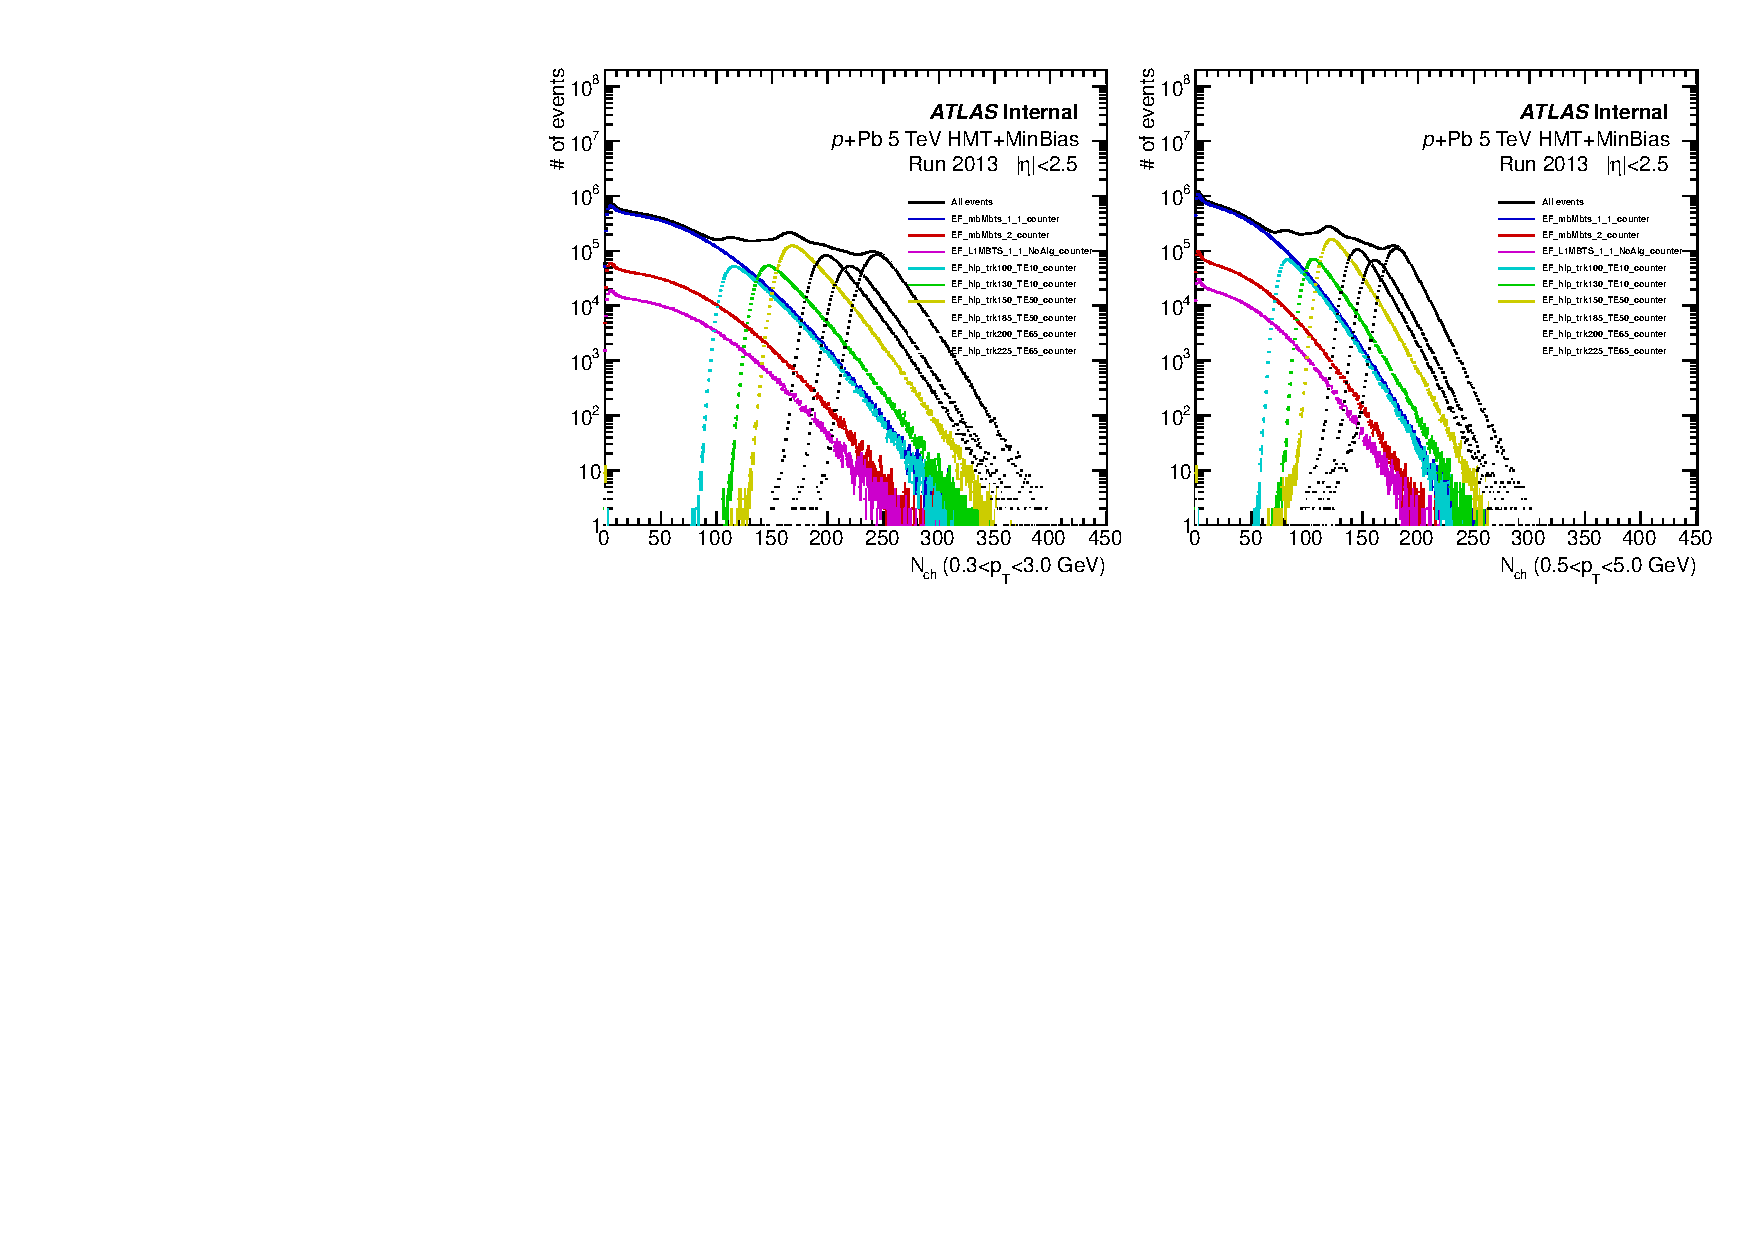
\includegraphics[width=.9\linewidth]{figs/sec_evtSlc/trkDis_pPb5_run1.pdf}
\caption{Distribution of number of tracks with two $p_{T}$ thresholds: $0.3<p_{T}<3.0$ GeV and $0.5<p_{T}<5.0$ GeV, in 5 TeV $p$+Pb run 2013. The major MinBias and HMT triggers are plotted separately.}
\label{fig:trkDis_pPb5_run1}
\end{figure}
The summary of statistics with all the major triggers used in this analysis are shown in Fig.~\ref{fig:trkDis_pPb5_run1}.

\begin{figure}[H]
\centering
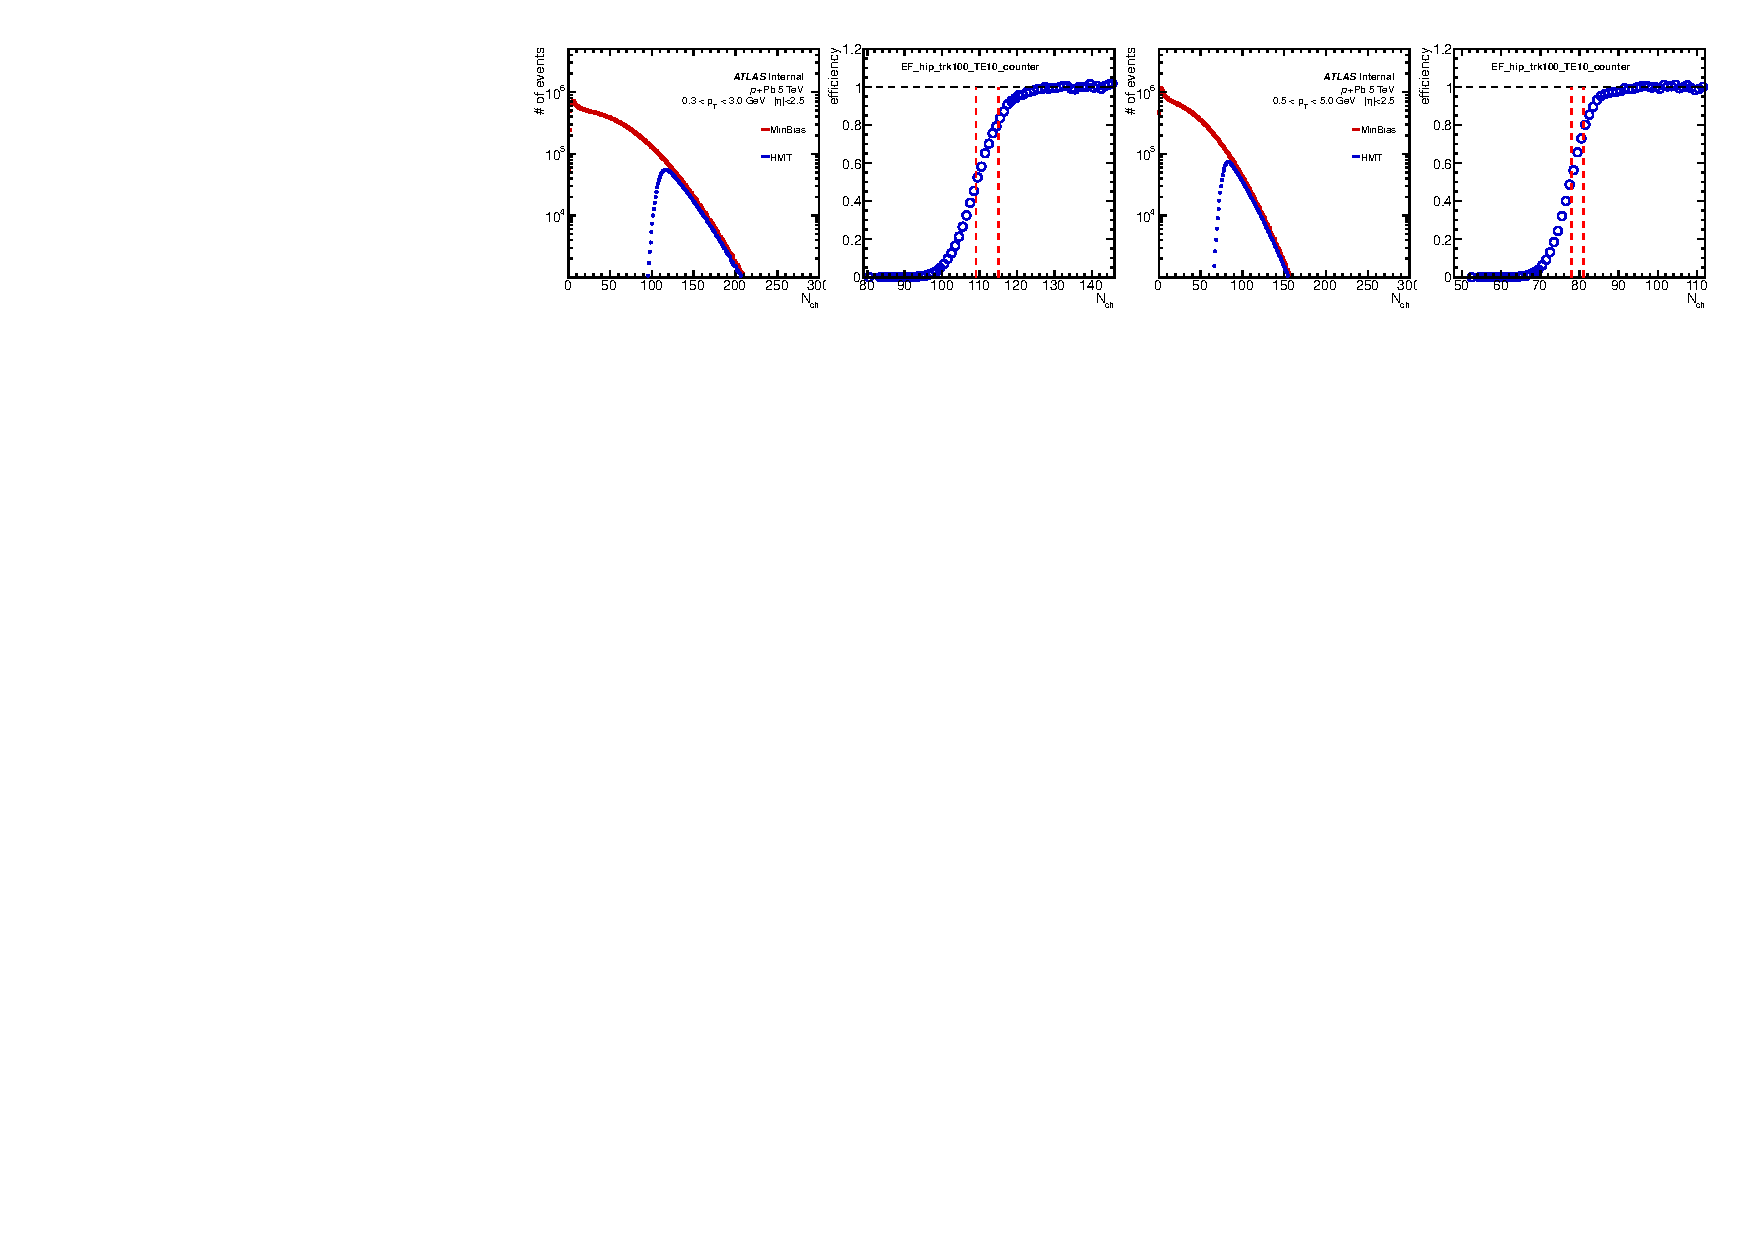
\includegraphics[width=1.\linewidth]{figs/sec_evtSlc/trigEff_pPb5_run1/trigEff_Trig8.pdf}
\end{figure}
\begin{figure}[H]
\centering
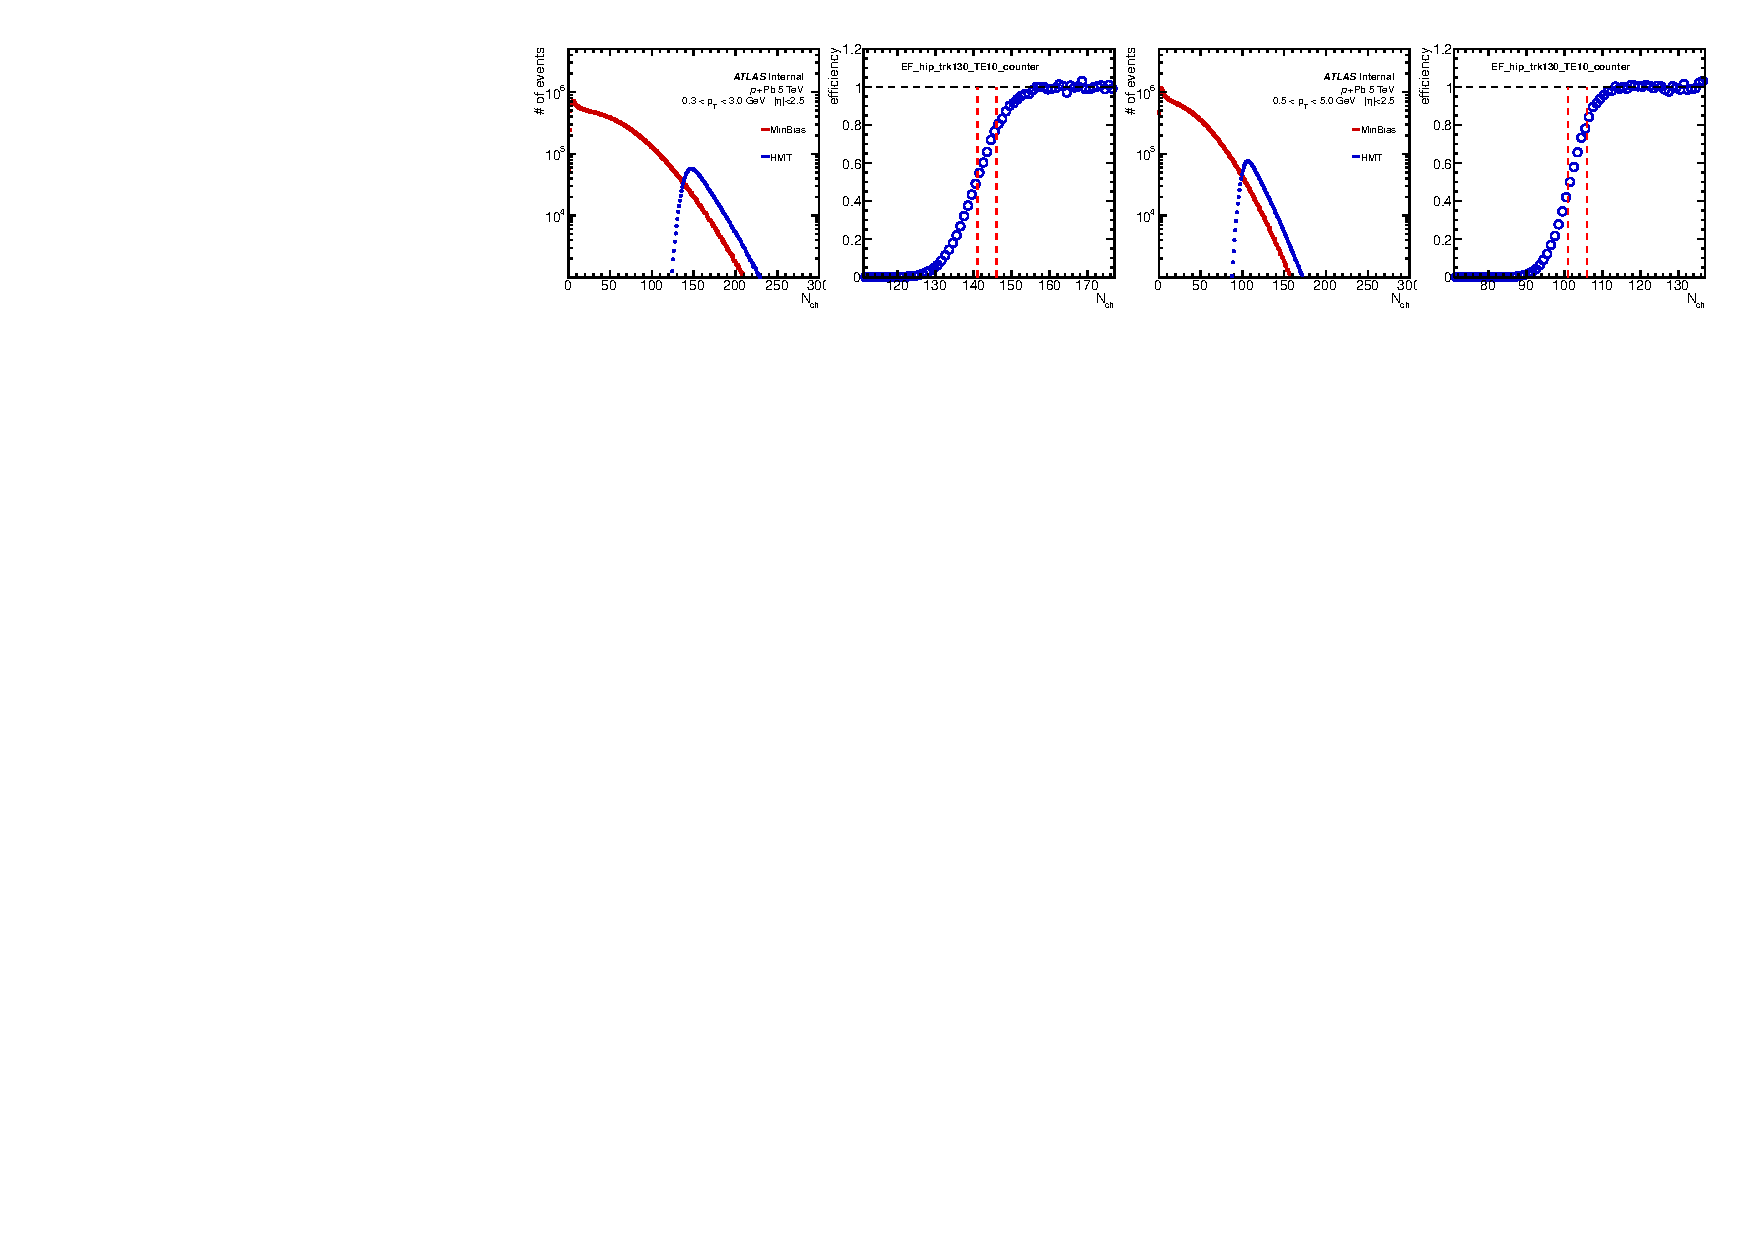
\includegraphics[width=1.\linewidth]{figs/sec_evtSlc/trigEff_pPb5_run1/trigEff_Trig9.pdf}
\end{figure}
\begin{figure}[H]
\centering
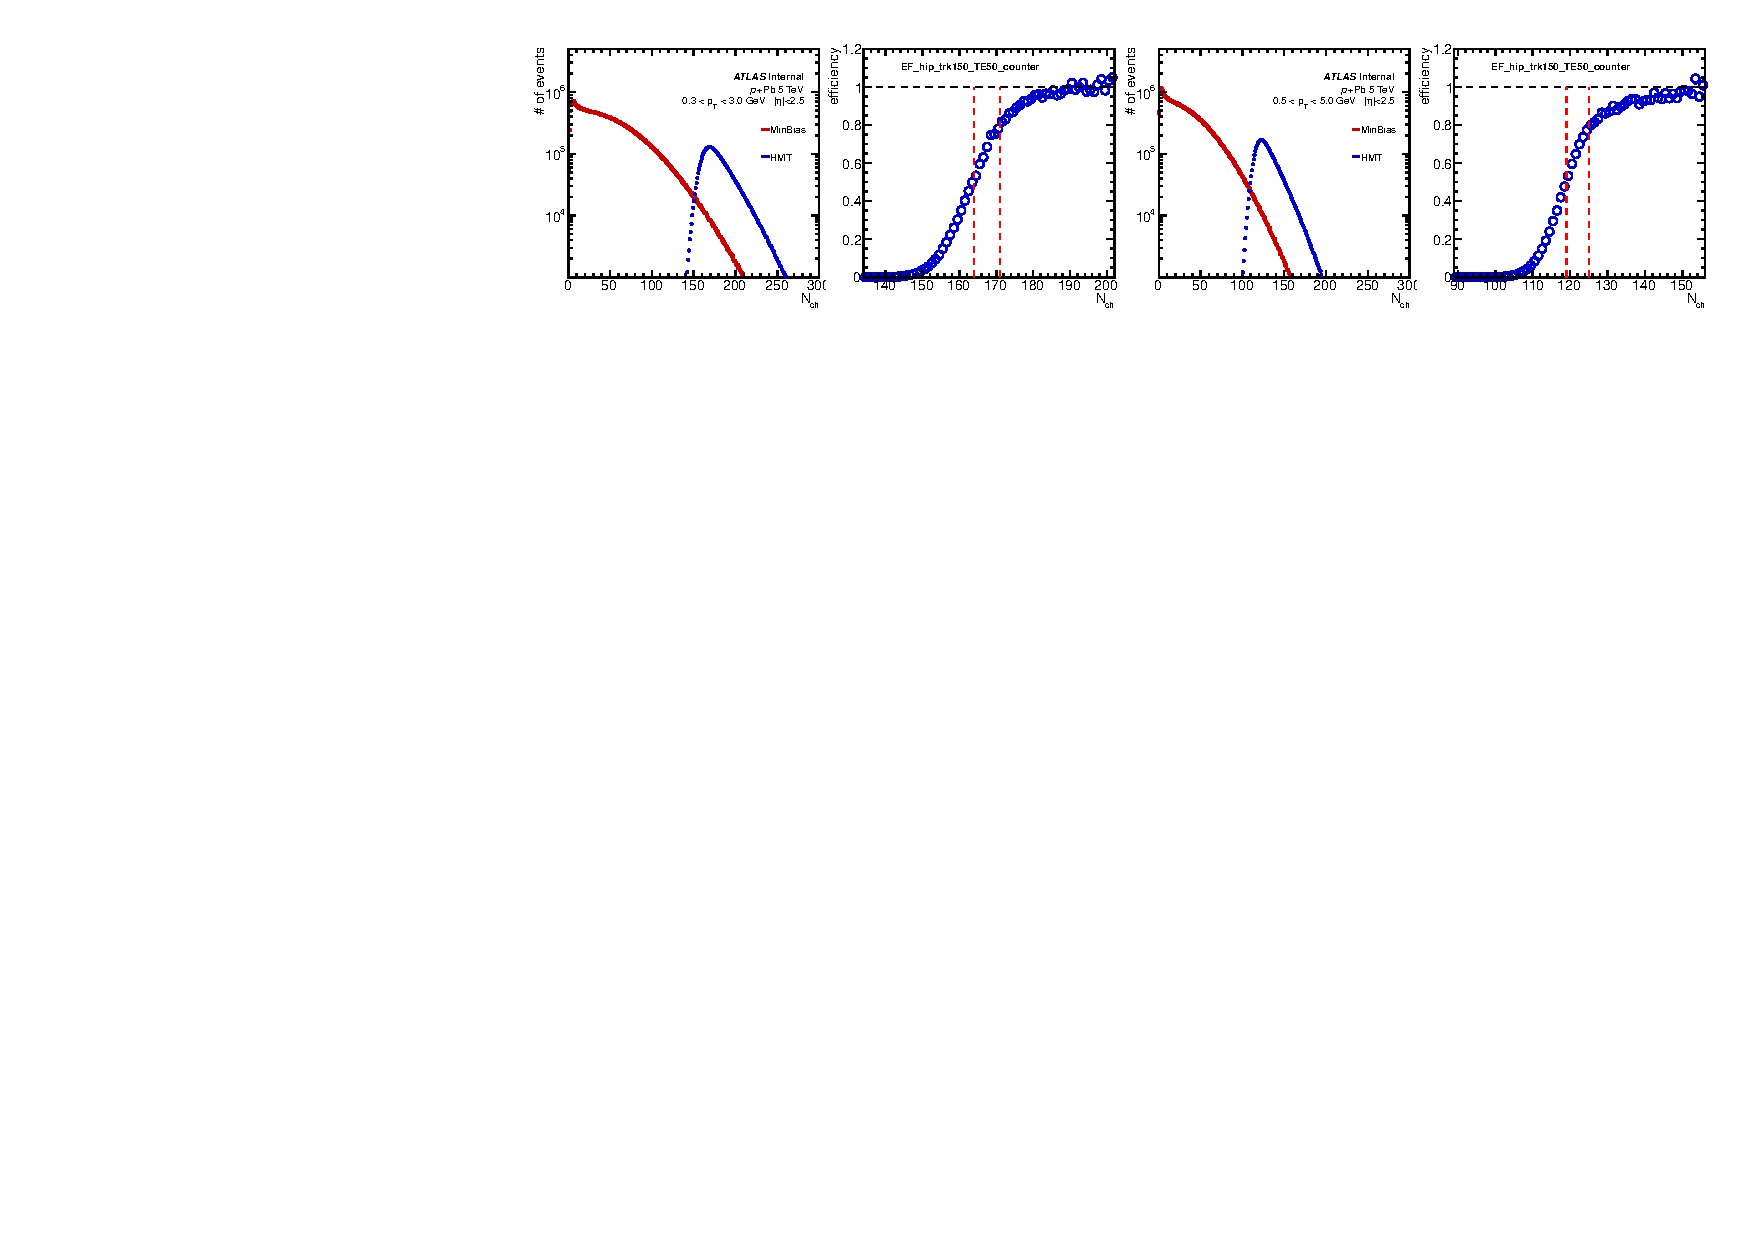
\includegraphics[width=1.\linewidth]{figs/sec_evtSlc/trigEff_pPb5_run1/trigEff_Trig10.pdf}
\end{figure}
\begin{figure}[H]
\centering
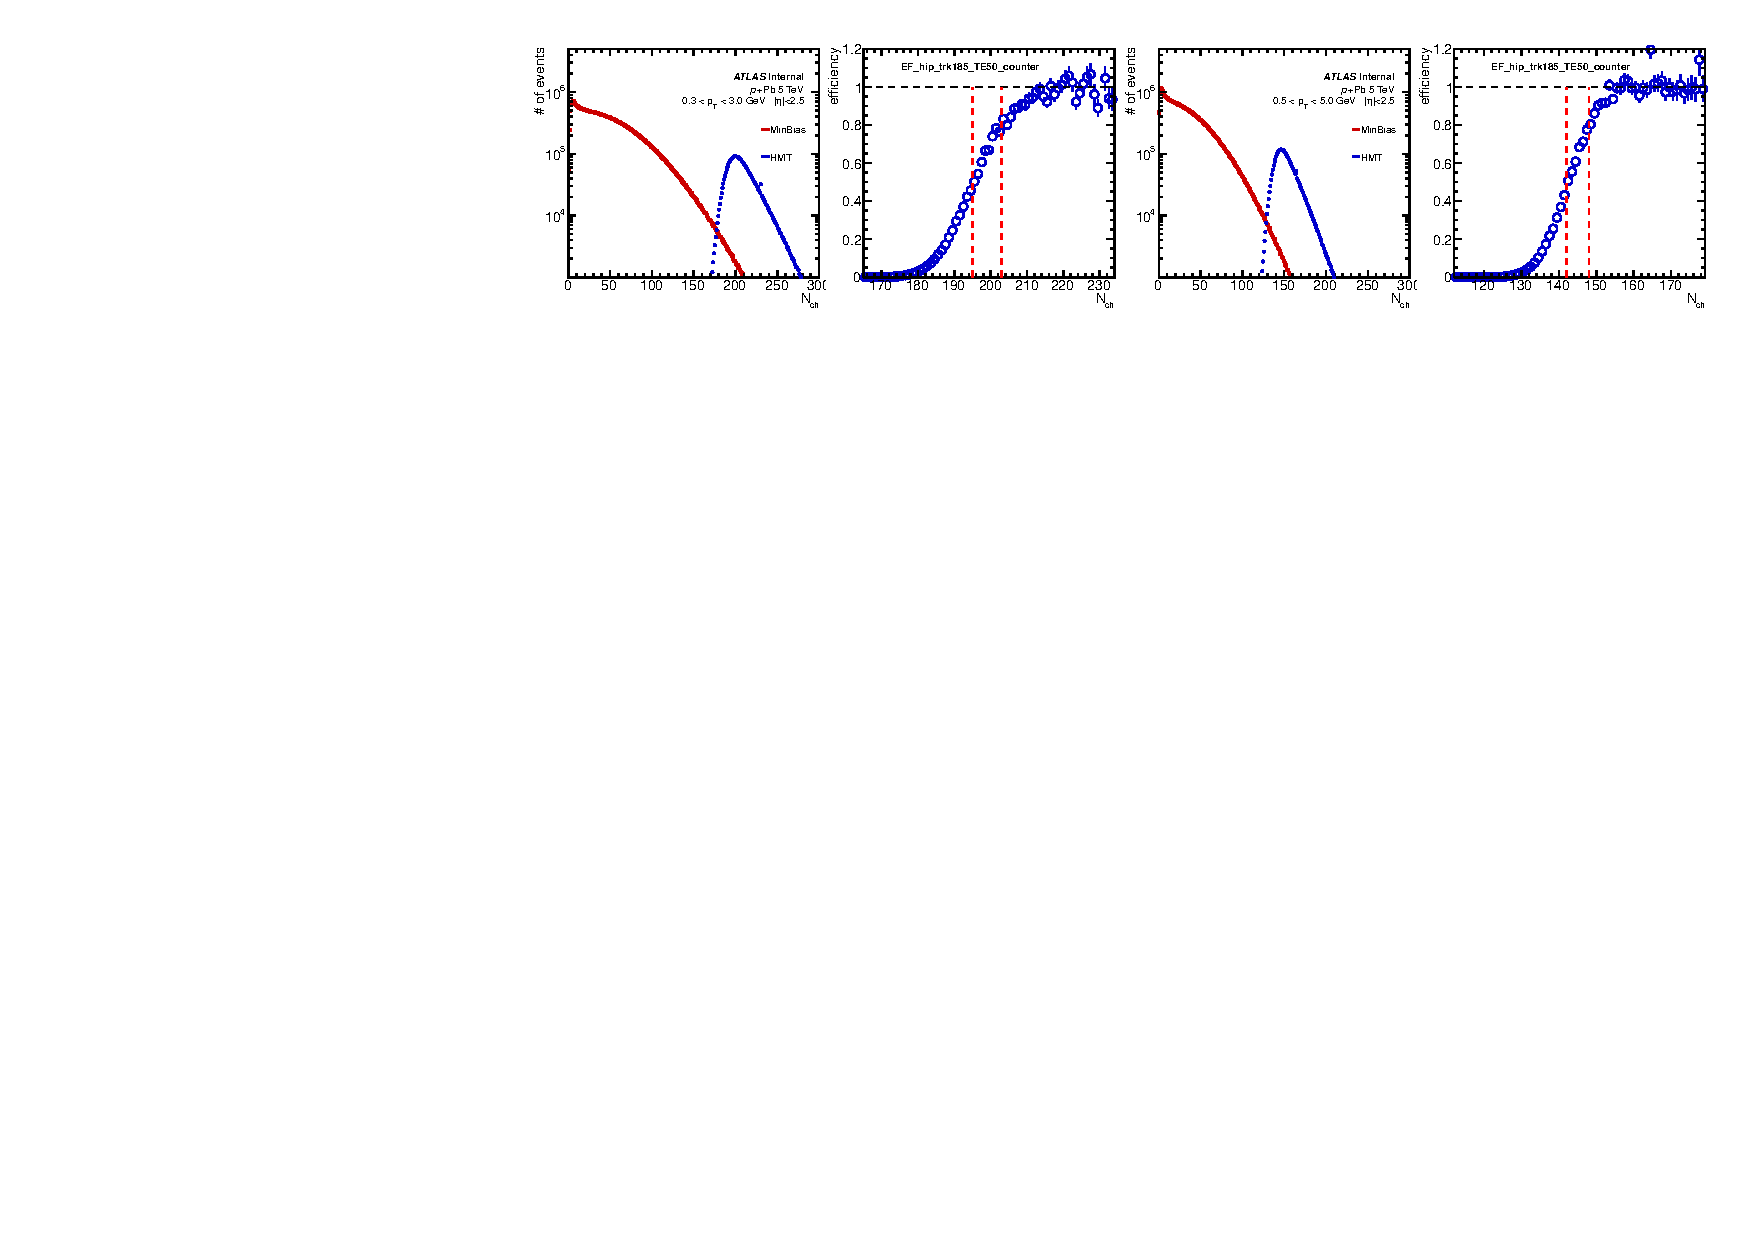
\includegraphics[width=1.\linewidth]{figs/sec_evtSlc/trigEff_pPb5_run1/trigEff_Trig11.pdf}
\end{figure}
\begin{figure}[H]
\centering
\includegraphics[width=1.\linewidth]{figs/sec_evtSlc/trigEff_pPb5_run1/trigEff_Trig12.pdf}
\end{figure}
\begin{figure}[H]
\centering
\includegraphics[width=1.\linewidth]{figs/sec_evtSlc/trigEff_pPb5_run1/trigEff_Trig13.pdf}
\caption{Trigger efficiencies of all major HMT triggers as a function of number of tracks in two $p_{T}$ ranges: $0.3<p_{T}<3.0$ GeV and $0.5<p_{T}<5.0$ GeV, from 5 TeV $p$+Pb run. Efficiency is calculated relative to the corresponding MinBias trigger in this run period then scaled to 1.0 in the large $N_{ch}$ region. The two red dash lines indicate 50$\%$ and 80$\%$ efficiency cuts.}
\label{fig:trigEff_pPb5_run1}
\end{figure}
Trigger efficiencies of all the major HMT triggers are summarized in Fig.~\ref{fig:trigEff_pPb5_run1}, where efficiencies are shown for two $p_{T}$ ranges separately: $0.3<p_{T}<3.0$ GeV and $0.5<p_{T}<5.0$ GeV.



\subsubsection{HIJING for 2013 $p$+Pb data}
Tracking efficiency and fraction of fake tracks have been extensively studied in previous $p$+Pb flow analyses~\cite{Aad:2014lta, atlas:3}. In this analysis we are re-using the efficiency map applied in the forward-backward multiplicity fluctuation paper \verb|ATL-COM-PHYS-2015-655|, where the tracking efficiency is estimated as a function of $\eta$, $p_{T}$, $N_{ch}$ and $z$ position of the vertex.



\subsubsection{2016 $p$+Pb}
In 2016, 5.02 TeV $p$+Pb data was collected with ATLAS detectors, with lower $\mu$ value than 2013. In additional to GRL selection, each event is required to have at least one vertex. Besides, problematic events are also removed:
\begin{itemize}
\item due to the liquid argon system
\item due to the tile calorimeter system
\item due to the SCT inner detector system
\item due to incomplete events (event information missing after TTC restarts)
\end{itemize}
and since the $\mu$ value of this year's run is much lower than 2013, cleaning pile-up events is not crucial. In the later section, with 2016 8.16 TeV $p$+Pb data, we will show that for events with $\mu<0.01$, pile-up effects are negligible.

Since this year's $p$+Pb run is right after the $pp$ run, the track selection criteria is identical to $pp$. An additional tighter $d_{0}$ and $z_{0}$ pointing cut is used to check the stability of results in the systematics section.

All the runs included in this analysis are listed as follows:
\begin{itemize}

\item Run 312649, 8.9 million events from MinBias stream
\begin{itemize}[leftmargin=*]
\item[] \verb|data16_hip5TeV.00312649.physics_Main.recon.AOD.f784_m1741|
\end{itemize}

\item Run 312796, 43 million events from MinBias stream
\begin{itemize}[leftmargin=*]
\item[] \verb|data16_hip5TeV.00312796.physics_Main.recon.AOD.f784_m1741|
\end{itemize}

\item Run 312837, 85 million events from MinBias stream
\begin{itemize}[leftmargin=*]
\item[] \verb|data16_hip5TeV.00312837.physics_Main.recon.AOD.f774_m1736|
\end{itemize}

\item Run 312937, 26 million events from MinBias stream
\begin{itemize}[leftmargin=*]
\item[] \verb|data16_hip5TeV.00312937.physics_Main.recon.AOD.f774_m1736|
\end{itemize}

\item Run 312945, 29 million events from MinBias stream
\begin{itemize}[leftmargin=*]
\item[] \verb|data16_hip5TeV.00312945.physics_Main.recon.AOD.f774_m1736|
\end{itemize}

\item Run 312968, 37 million events from MinBias stream
\begin{itemize}[leftmargin=*]
\item[] \verb|data16_hip5TeV.00312968.physics_Main.recon.AOD.f774_m1736|
\end{itemize}

\item Run 314199, 240 million events from MinBias stream
\begin{itemize}[leftmargin=*]
\item[] \verb|data16_hip5TeV.00314199.physics_Main.recon.AOD.f781_m1741|
\end{itemize}

\end{itemize}

Due to the reason that the intermediate $N_{ch}$ region is not covered by HMT triggers, several HMT triggers with intermediate $N_{ch}$ thresholds are specially designed before 2016 data taking. Together with MinBias triggers, all the major triggers used in this analysis is summarized as follows:
\begin{itemize}
\item \verb|HLT_noalg_mb_L1MBTS_1|
\item \verb|HLT_noalg_mb_L1MBTS_1_1|
\item \verb|HLT_mb_sp100_trk10_hmt_L1MBTS_1_1|
\item \verb|HLT_mb_sp100_trk20_hmt_L1MBTS_1_1|
\item \verb|HLT_mb_sp100_trk30_hmt_L1MBTS_1_1|
\item \verb|HLT_mb_sp100_trk60_hmt_L1MBTS_1_1|
\item \verb|HLT_mb_sp100_trk80_hmt_L1MBTS_1_1|
\item \verb|HLT_mb_sp100_trk100_hmt_L1MBTS_1_1|
\item \verb|HLT_mb_sp100_trk110_hmt_L1MBTS_1_1|
\end{itemize}
where all the HMT triggers are seeded on \verb|L1MBTS_1_1|, which is different from 2013 since the luminosity is much lower.

\begin{figure}[H]
\centering
\includegraphics[width=.9\linewidth]{figs/sec_evtSlc/trkDis_pPb5_run2.pdf}
\caption{Distribution of number of tracks with two $p_{T}$ thresholds: $0.3<p_{T}<3.0$ GeV and $0.5<p_{T}<5.0$ GeV, in 5 TeV $p$+Pb run 2016. The major MinBias and HMT triggers are plotted separately.}
\label{fig:trkDis_pPb5_run2}
\end{figure}
The summary of statistics with all the major triggers used in this analysis are shown in Fig.~\ref{fig:trkDis_pPb5_run2}.

\begin{figure}[H]
\centering
\includegraphics[width=1.\linewidth]{figs/sec_evtSlc/trigEff_pPb5_run2/trigEff_Trig6.pdf}
\end{figure}
\begin{figure}[H]
\centering
\includegraphics[width=1.\linewidth]{figs/sec_evtSlc/trigEff_pPb5_run2/trigEff_Trig8.pdf}
\end{figure}
\begin{figure}[H]
\centering
\includegraphics[width=1.\linewidth]{figs/sec_evtSlc/trigEff_pPb5_run2/trigEff_Trig10.pdf}
\end{figure}
\begin{figure}[H]
\centering
\includegraphics[width=1.\linewidth]{figs/sec_evtSlc/trigEff_pPb5_run2/trigEff_Trig11.pdf}
\caption{Trigger efficiencies of all major HMT triggers as a function of number of tracks in two $p_{T}$ ranges: $0.3<p_{T}<3.0$ GeV and $0.5<p_{T}<5.0$ GeV, from 2016 5 TeV $p$+Pb run. Efficiency is calculated relative to the corresponding MinBias trigger in this run period then scaled to 1.0 in the large $N_{ch}$ region. The two red dash lines indicate 50$\%$ and 80$\%$ efficiency cuts.}
\label{fig:trigEff_pPb5_run2}
\end{figure}
Trigger efficiencies of all the major HMT triggers are summarized in Fig.~\ref{fig:trigEff_pPb5_run2}, where efficiencies are shown for two $p_{T}$ ranges separately: $0.3<p_{T}<3.0$ GeV and $0.5<p_{T}<5.0$ GeV.



\subsubsection{HIJING for 2016 $p$+Pb data}
By comparing Fig.~\ref{fig:trkDis_pPb5_run1} and Fig.~\ref{fig:trkDis_pPb5_run2}, it is obvious that 2016 collected much more statistics than 2013 in low and intermediate $N_{ch}$ region. Since cumulant measurement is dominated by statistics errors, 2016 5 TeV $p$+Pb data will be included in this analysis. There existed 1 million HIJING~\cite{Gyulassy:1994ew} sample before this year's run with Run 2 configuration. In this section, we will show the this HIJING sample is sufficient for the tracking efficiency estimation.

\begin{figure}[H]
\centering
\includegraphics[width=0.9\linewidth]{figs/sec_evtSlc/MC_pPb5_ev1_Nch0.pdf}
\includegraphics[width=0.9\linewidth]{figs/sec_evtSlc/MC_pPb5_ev1_Nch1.pdf}
\caption{Tracking efficiency as a function of $\eta$ and $p_{\text{T}}$. Top three panels are estimated in $N_{ch}<100$ and bottom panels are for $N_{ch}>100$. The 1st column is the tracking efficiency estimated from PYTHIA with Run 2 configuration; 2nd column is from the HIJING sample before 2016 5 TeV $p$+Pb run and 3rd column is the ratio between HIJING and PYTHIA.}
\label{fig:MC_pPb5_ev1}
\end{figure}
Fig.~\ref{fig:MC_pPb5_ev1} shows the comparisons of tracking efficiencies as a function of $\eta$ and $p_{\text{T}}$. Based on the ratio plot, even though tracking efficiencies are estimated from PYTHIA and HIJING, since both the Monte-Carlo samples have Run 2 configurations, the relative differences are within $2\%$ for $N_{ch}<100$. For $N_{ch}>100$, the relative difference is larger because of larger statistical errors in larger $N_{ch}$ region. This result means that the tracking efficiency stays stable in Run 2, from Year 2015 to 2016. Thus one should not expect big changes for 2016 $p$+Pb data.

\begin{figure}[H]
\centering
\includegraphics[width=0.9\linewidth]{figs/sec_evtSlc/MC_pPb5_ev2_raw.pdf}
\includegraphics[width=0.9\linewidth]{figs/sec_evtSlc/MC_pPb5_ev2_crr.pdf}
\caption{Particle distribution as a function of $N_{ch}$ and $p_{\text{T}}$. Top three panels are the raw distribution while bottom three panels are weighted by inverse of the tracking efficiency. The 1st column is from 2013 5 TeV $p$+Pb, 2nd column is from 2016 5 TeV $p$+Pb and 3rd column is the ratio between 2016 and 2013.}
\label{fig:MC_pPb5_ev2}
\end{figure}
Fig.~\ref{fig:MC_pPb5_ev2} shows the comparison of particle distributions as a function of $N_{ch}$ and $p_{\text{T}}$, using 2013 and 2016 5 TeV $p$+Pb data. From ratio of raw distributions, 2016 data reconstructs $5\%$ more tracks in the lowest $p_{\text{T}}$ region. The reason is that in Run 2, IBL was implemented to the inner detector, which provides better tracking reconstruction in lower $p_{\text{T}}$ region. Meanwhile, once the particles are weighted by the inverse of tracking efficiencies, the difference reduces down to $2\%$. This means the HIJING sample we used correctly estimated the tracking efficiency in the new data, since one should not expect any difference between the $p_{\text{T}}$ spectrum from 2013 and 2016. The remaining $1\%$ to $2\%$ difference in the lowest $p_{\text{T}}$ region is negligible since in the systematic checks of tracking efficiency, a difference on the level of $10\%$ has been evaluated and included as one of the systematics.

\begin{figure}[H]
\centering
\includegraphics[width=0.45\linewidth]{figs/sec_evtSlc/MC_pPb5_ev3_mtd0}
\includegraphics[width=0.45\linewidth]{figs/sec_evtSlc/MC_pPb5_ev3_mtd1}
\caption{Comparison of $C_{2}\{4\}$ measured in 2013 and 2016 5 TeV $p$+Pb data, with traditional method (left) and 3 sub-event method (right). Particles have $0.3<p_{\text{T}}<3.0$ GeV.}
\label{fig:MC_pPb5_ev3}
\end{figure}
Last but not least, it is worthwhile to directly compare the physics observable using 2013 and 2016 data, with tracking efficiency correction. As shown in Fig.~\ref{fig:MC_pPb5_ev3}, $C_{2}\{4\}$ measured in the 2013 and 2016 are consistent within statistical errors, for both traditional and 3 sub-event methods. With all the three evidences listed above, we decide to use this mentioned HIJING sample to estimate tracking efficiency and 2016 5 TeV $p$+Pb has been included in the final results.


















